\documentclass{ucbthesis}
% ^^ change to \documentclass{ucbthesis} if this is for PhD

\usepackage[sorting=none,backend=bibtex]{biblatex}
 %\usepackage[backend=bibtex,style=verbose-trad2] 
\usepackage{algorithm}
\usepackage{algpseudocode}
\usepackage{graphicx}
\usepackage{scrextend}
\usepackage{amsmath}
\usepackage{multirow}

% Double spacing, if you want it.
% \def\dsp{\def\baselinestretch{2.0}\large\normalsize}
% \dsp

% If the Grad. Division insists that the first paragraph of a section
% be indented (like the others), then include this line:
% \usepackage{indentfirst}

%%%%%%%%%%%%%%%%%%
% If you want to use "sections" to partition your thesis
% un-comment the following:
% 
% \counterwithout{section}{chapter}
% \setsecnumdepth{subsubsection}
% \def\sectionmark#1{\markboth{#1}{#1}}
% \def\subsectionmark#1{\markboth{#1}{#1}}
% \renewcommand{\thesection}{\arabic{section}}
% \renewcommand{\thesubsection}{\thesection.\arabic{subsection}}
% \makeatletter
% \let\l@subsection\l@section
% \let\l@section\l@chapter
% \makeatother
% 
% \renewcommand{\thetable}{\arabic{table}}
% \renewcommand{\thefigure}{\arabic{figure}}
%
%%%%%%%%%%%%%%%%%%

\newtheorem{theorem}{Jibberish}

%\newtheorem{theorem}{Theorem}[section]
\newtheorem{lemma}[theorem]{Lemma}
\newtheorem{proposition}[theorem]{Proposition}
\newtheorem{corollary}[theorem]{Corollary}

\newenvironment{proof}[1][Proof]{\begin{trivlist}
\item[\hskip \labelsep {\bfseries #1}]}{\end{trivlist}}
\newenvironment{definition}[1][Definition]{\begin{trivlist}
\item[\hskip \labelsep {\bfseries #1}]}{\end{trivlist}}
\newenvironment{example}[1][Example]{\begin{trivlist}
\item[\hskip \labelsep {\bfseries #1}]}{\end{trivlist}}
\newenvironment{remark}[1][Remark]{\begin{trivlist}
\item[\hskip \labelsep {\bfseries #1}]}{\end{trivlist}}

\newcommand{\qed}{\nobreak \ifvmode \relax \else
      \ifdim\lastskip<1.5em \hskip-\lastskip
      \hskip1.5em plus0em minus0.5em \fi \nobreak
      \vrule height0.75em width0.5em depth0.25em\fi}
\algnewcommand{\LineComment}[1]{\State \(\triangleright\) #1}


\bibliography{IEEEabrv,references}

\hyphenation{mar-gin-al-ia}

\begin{document}

% Declarations for Front Matter

\title{Accelerator Synthesis and Integration for CPU FPGA Systems }
\author{Shaoyi Cheng}
\degreesemester{Spring}
\degreeyear{2016}
\degree{Doctor of Philosophy}
\chair{Professor John Wawrzynek}
\othermembers{Professor Krste Asanovic \\
  Professor Dorit Hochbaum}
\numberofmembers{3}
\prevdegrees{B.ASc. (University of Toronto) 2009 \\
  M.S. (University of California, Berkeley) 2012}
\field{Computer Science}
\campus{Berkeley}


% The title page generated by LaTeX is now acceptable for handing in.
% (This was not always the case).

\maketitle

\approvalpage
% ^^ comment this out when compiling your final draft

\copyrightpage

% (This is included by thesis.tex; you do not latex it by itself.)

\begin{abstract}

% The text of the abstract goes here.  If you need to use a \section
% command you will need to use \section*, \subsection*, etc. so that
% you don't get any numbering.  You probably won't be using any of
% these commands in the abstract anyway.
As the scaling down of transistor sizing no longer provides boost to processor clock frequency, there has been
a move towards parallel computers and more recently, heterogeneous
computing platforms.
To target the FPGA component in these systems, high-level synthesis (HLS) tools are developed to facilitate hardware generation from higher level algorithmic descriptions.
Despite being an effective method for rapid hardware generation,
in the context of offloading compute intensive software kernels
to FPGA accelerators, current HLS tools do not always take
full advantage of the hardware platforms. Processor centric software implementations often have to be rewritten if good quality of results is desired.



%As high-level synthesis (HLS) moves towards mainstream adoption among FPGA designers, it has proven to be an effective method for rapid hardware generation. However, in the context of offloading compute intensive software kernels to FPGA accelerators, current HLS tools do not always take full advantage of the hardware platforms. Processor centric software implementations often have to be rewritten if good quality of results is desired.

In this work, we present a framework to refactor and restructure compute intensive software kernels, making them better suited
for FPGA platforms. An algorithm was proposed to
decouple memory operations and computation, generating accelerator pipelines composed of
independent modules connected through FIFO channels.
These decoupled computational pipelines have much better throughput due to their efficient use of the memory bandwidth and improved tolerance towards data access latency.
Our methodology complements existing work in high-level synthesis and facilitates the creation of heterogeneous
systems with high performance accelerators and general purpose
processors. With our approach, for a set of non-regular algorithm
kernels written in C, a performance improvement of 3.3 to 9.1x
is observed over direct C-to-Hardware mapping using a state-of-the-art HLS tool.

To ensure the absence of artificial deadlocks in the pipeline generated by our framework, we also formulated an analysis scheme examining various dependencies between operations distributed across different pipeline modules. The interactions between the modules' schedules, the capacity of the communication channels and the memory access mechanisms are all incorporated
into our model, such that potential artificial deadlocks can be detected and resolved \textit{a priori}. The applicability of our technique is not limited to the computational pipeline generated
by our algorithm, but also other networks of communicating processes if their interaction with the channels follows a set of simple rules.

%Using the newly developed flow, we explore how to minimize user effort in generating and integrating FPGA accelerator with the CPU running software.
To push the limit in usability of FPGA platforms, we also explored the generation and integration of accelerators using only program binaries and execution profiles. Assuming no user input, the approach is only applied to more regular applications,
%It makes the FPGA completely 
%transparent to the user and can be used even in the absence of source code. 
%Of course, the scope of applications this approach can be applied to is relatively narrow. Only regular computation kernels can be converted to FPGA accelerators.
%This approach is only beneficial for more regular applications,
where the memory access patterns are analyzable and coarse grained paralellism can be extracted. A run time mechanism is also devised
to ensure the correctness of the parallelization performed during accelerator synthesis. With the help of binary instrumentation tools, it becomes possible to integrate the FPGA-accelerated parts into the original application in a user transparent way. Neither recompilation of the original program nor the source code is required.
This approach is applied to a few benchmarks for which decoupled computational pipelines are synthesized. With memory level and coarse grained parallelization, significant improvement in performance (3.7 to 9x) over general purpose processor was observed, despite the FPGA running at a fraction of the CPU's clock frequency. The run time checking mechanism was also shown to only incur small overhead, especially for loop nests with large number of iterations. 

%Using the computational pipeline synthesis flow  developed in this work, we applied this approach to a few benchmarks. The coarse grained parallelization provides significant improvement in performance over general purpose processor and the run time checking mechanism is shown to only incur small overhead, especially for loop nests with large number of iterations.
%Performing all the analysis based on program binary does introduce more uncertainty
%than a source code based approach. Thus we have devised a two phase mechanism to have parts of the 
%analysis done during the runtime to ensure correctness. The details are described

\begin{comment}

%much better performance. 
%much better throughput due to their
%efficient use of the memory bandwidth and improved tolerance
%to data access latency. 
The methodology complements existing
work in high-level synthesis, easing the creation of heterogeneous
systems with high performance accelerators and general purpose
processors. With this approach, for a set of non-regular algorithm
kernels written in C, a performance improvement of 3.3 to 9.1x
is observed over direct C-to-Hardware mapping using a state-ofthe-art
HLS tool.

general framework for
transforming a sequential program into a network of processes, which are then
converted to hardware accelerators through high level synthesis.
Also proposed is a complementing technique for performing static deadlock analysis of the generated accelerator network.
The interactions between the accelerators' schedules, the capacity of the communication
channels in the network and the memory access mechanisms are all incorporated
into our model, such that potential artificial deadlocks can be detected and resolved \textit{a priori}.
\end{comment}
\end{abstract}


\begin{frontmatter}

\begin{dedication}
\null\vfil
\begin{center}
To Me\\\vspace{12pt}
\end{center}
\vfil\null
\end{dedication}

\tableofcontents
\clearpage
\listoffigures
\clearpage
\listoftables
\clearpage


\begin{acknowledgements}
I want to thank my advisor for advising me.
\end{acknowledgements}

\end{frontmatter}

\pagestyle{headings}

% (Optional) \part{First Part}

\chapter{Introduction}
\label{chap1}
\section{Trend in General Purpose Computing Platforms}
The downscaling of transistor size, as first observed by Moore~\cite{Moore:2000:CMC:333067.333074}, massively increased the
capability of VLSI circuits for more than three decades. The number of transistors on a single silicon die doubles approximately every 18 months while the supply voltage and transistor channel length scaled down according to the prediction by Dennard~\cite{dennard1974design}. This advancement in technology not only
enabled more integration, it also kept the power consumption of the new chip the same as its predecessors, taking advantage of the voltage scaling. Bigger caches and
various architectural features were implemented using the newly available
transistors, which improved single thread performance. At the same time, the voltage scaling also allows for increased clock frequency of processors under the same power budget. Intel 80386 chips released in the 80s operated at 25 MHz while the Pentium D, released in the middle of the last decade, reached
a clock frequency of more than 3.5 GHz. This 140x boost in frequency, coupled with
greater instruction issue width, more accurate branch predictor and many other
micro-architectural innovations unlocked huge performance increase for
software applications during this period. No change in programming methodology
was needed to harness the ever increasing power of the new processors.  Unfortunately, the leakage current quickly grows as the threshold voltage of transistor decreases. Eventually,
further scaling of the supply voltage was no longer possible and with that, the clock rate of the mainstream processors stagnated at approximately 3.8 GHz. 


%\section{Trend Towards Heterogeneity}
As the growth of processor clock frequency came to a stop in the middle of the last decade,
the performance boost provided by the continuous advancement of hardware technology for sequential programs
can no longer be sustained. The benefits of user transparent architecture optimizations are also 
diminishing. As parallel computers and more recently, heterogeneous computing platforms become mainstream,
the software developers are finally faced with the challenge of matching their computation specifications
with the characteristics of the underlying compute substrate. 


\begin{figure}[htp]
\begin{center}
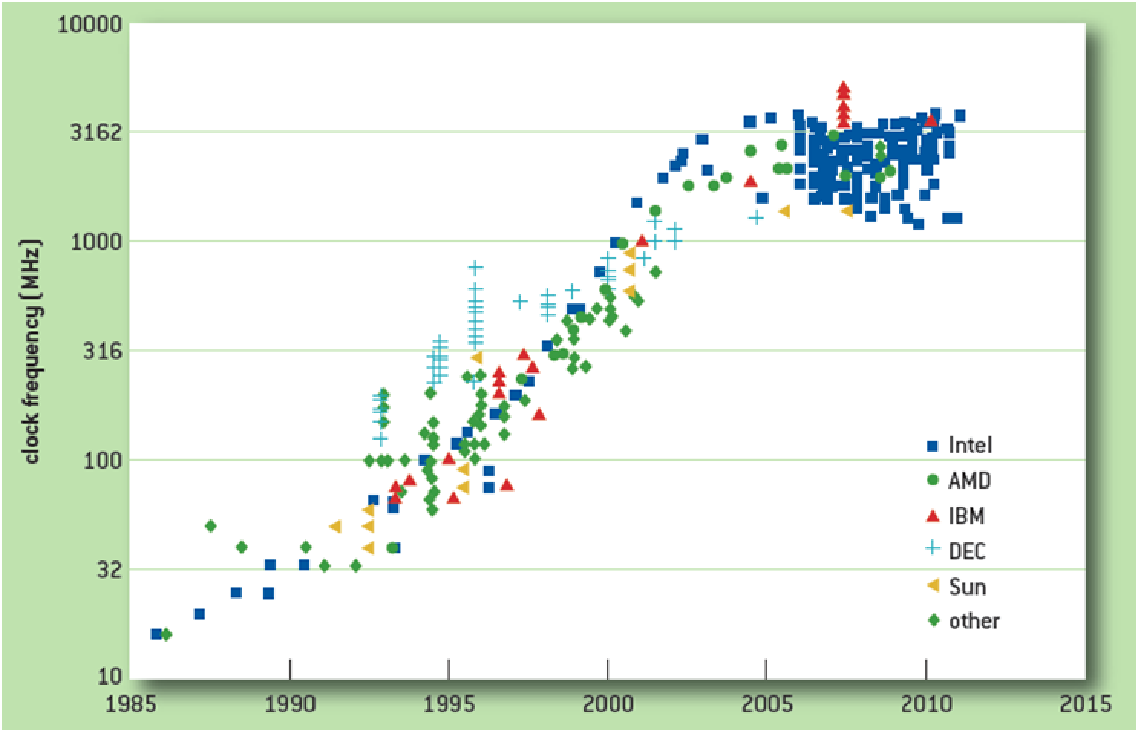
\includegraphics[width=0.6\linewidth]{chap1fig/cpuscaling.pdf}
\caption{Processor Frequency Scaling Over Time~\cite{Danowitz:2012:CDR:2133806.2133822}
\label{fig:cpuscaling}}
\end{center}
\end{figure}

During the rise of 
parallel computer systems, the research community created many auto parallelization tools~\cite{Wilson:1994:SCS:891422}~\cite{Blume94polaris:the}~\cite{oscar},
to relieve the programmers from the tedious manual parallelization process. As real applications
often contain irregular algorithms which are hard to analyze, various
mechanisms were also proposed for users to provide hints/interactively guide the parallelizing compiler~\cite{RiceUniversity:1993:HPF:174223.158909}~\cite{Liao:1999:SEI:329366.301108}~\cite{86108}.
% 
A very similar trend, is currently happening in the heterogeneous computing realm as well.



\section{Heterogeneous Computing with Field Programmable Gate Arrays}
\label{chap1:het}
Field programmable gate array (FPGA) is a fundamentally different computation device
compared to the conventional microprocessors. Figure~\ref{fig:fpgaArch}
shows a simple FPGA which contains a matrix
of logic blocks connected by programmable interconnect. Each logic block
can be configured to perform different compute operations while the interconnect links them together to form a fixed function hardware engine.
Compare to application specific integrated circuits(ASICs), the FPGA configurations can be easily changed to implement many different functions,
accommodating various needs of the users.
This flexibility of course comes at a cost. As the logic and
routing resources are all reprogrammable mechanisms supported by RAM bits, there are significant
area, performance and power overheads compared to the ASICs~\cite{4068926}. To alleviate these disadvantages, 
more specialized circuits like block RAM and DSP blocks are added to modern
FPGAs~\cite{chips:virtex5}~\cite{chips:arria}. Subsequently some of the common functions can be mapped onto
these blocks and get closer to ASIC performance/power. When an application
is implemented on an FPGA, arithmetic and logic operations are spatially mapped to
the various compute resources in the reconfigurable array, while the dependencies between them
are satisfied by physical connections formed with on-chip routing resources. Compare to the CPUs, where the ALUs are heavily time
multiplexed, FPGAs can perform orders of magnitude more operations every clock cycle due to its
massive parallelism. For the right kind of computation, FPGAs offer an attractive
trade-off between flexibility and efficiency compared to ASICs and CPUs, and
thus occupy a unique space in the spectrum of computing devices.

%The actual performance achievable certainly depends 
%on the nature of the application. Inherently serial functions may not be
%able to make use of abundance of computing resources and can have better
%speed on CPUs, due to the high clock frequency.


\begin{figure}[htp]
\begin{center}
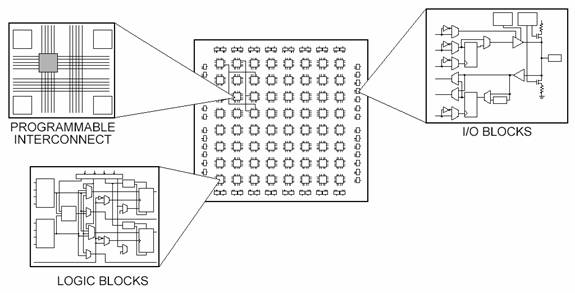
\includegraphics[width=0.8\linewidth]{chap1fig/archsim.jpg}
\caption{Simplified FPGA Architecture~\cite{fpgafun}
\label{fig:fpgaArch}}
\end{center}
\end{figure}

When CPUs are combined with FPGAs,
the resulted heterogeneous platforms would allow the users to place workloads onto the most appropriate
computing device to increase overall system efficiency.
Inherently serial functions may not be able to make use of the FPGAs' abundance of computing resources and can have better speed on the CPUs, due to its high clock frequency.
Meanwhile, functions with plenty of parallelism can take advantage of the
spatial computing paradigm provided by the FPGAs.
Application specific accelerators implementing these functions can offer
%with their tremendous flexibility, can be configured into application-specific
%accelerators which offer 
huge performance and energy advantages over general purpose
processors. There are many systems where FPGAs are coupled to CPUs through PCIe interconnect, Front Side Bus etc.~\cite{nallatech510T}~\cite{maxeler},
used in application domains ranging from scientific computing, gas and oil exploration to financial analytics
~\cite{smith2005scientific}~\cite{5719584}~\cite{6299067}.
Also, recent developments in FPGA SoCs, where the reconfigurable arrays are  integrated with hard processors and memory interface IPs at the chip level,
have created some highly compact yet versatile computing platforms~\cite{chips:zynq}~\cite{chips:cyclonesoc}. 
However, to make these platforms easily accessible to the application developers, there are still many challenges,
as the programming methodology for FPGAs is rather different than that for the general purpose processors.

%When applications are implemented on FPGAs, arithmetic and logic operations are spatially mapped to
%the various compute resources in the reconfigurable array, while the dependencies between them
%are satisfied by physical connections formed with on-chip routing resources. %Compare to the CPUs, where the ALUs are heavily time
%multiplexed, FPGAs can perform orders of magnitude more operations every clock cyle due to its
%massive parallelism. 
Traditionally, FPGAs are programmed using register transfer level (RTL) design
abstraction. The designers not only have to extract both coarse-grain and fine-grain parallelism in the
application, but also
need to define the behavior of the final implementation down to every clock cycle.
Hardware design principles such as clock management, state machines,
pipelining, and device specific memory management must be employed to really unlock the potential
in FPGA computing. All these concepts are unfortunately outside the expertise of most application-oriented
software developers. 

\section{High Level Synthesis} 
\label{chap1:hls}
Given the difficulty in programming FPGAs, there has
been a trend towards design synthesis from higher levels of
specifications~\cite{Coussy:2008:HSA:1457713},~\cite{intro2hls}. Being more compact and expressive, high level
languages, when used as design input, can greatly increase the
productivity of engineers. Just like in the case of parallelizing compilers, the gap between
an efficient implementation and a productive programming experience attracted major interest from 
both industry and academia. Many commercial,~\cite{tools:autoesl},~\cite{tools:catapultc}~\cite{tools:alterac2h},~\cite{tools:vivadohls} and open source~\cite{tools:legup},~\cite{tools:roccc} tools have been developed over the years 
to tackle this challenge of generating hardware functional blocks from high level
behavioral descriptions. Programming languages such as C/C++, designed for processor-centric execution, are used by these high-level synthesis programs as the medium for input specification. 

All these HLS tools attempt to capture parallelism in the control dataflow described by high level languages, often with various forms of guidance provided by the user, and 
generate hardware in the form of RTL.
Compute operations and memory accesses are allocated and scheduled according to the dependency constraints extracted
from analysis and resource constraints imposed by the target platform. The circuits generated usually follow
a Finite State Machine with Datapath (FSMD) paradigm. Activation of a particular operator in the datapath is associated
with a certain clock cycle and the execution of the entire control dataflow graph is orchestrated by 
a synthesized central controller. Depending on the system architecture, the generated hardware can have
different mechanisms in accessing the memory.
In some systems, direct memory access(DMA) engines are instantiated and data movements are explicitly managed, while 
%In the context of a CPU+accelerator system, 
in others, the generated
hardware is presented with a memory interface rather similar to that used by a processor, with various
caching schemes~\cite{6239785}~\cite{6239808} proposed to complement the datapath.

With the HLS tools, it seems the programmers now have an easy path to offloading the compute intensive parts of their software
to FPGAs, but the performance boost and energy efficiency of the mapped implementations are
often less than ideal. 
%The barrier between software and the reconfigurable fabric is more than just the language used, the
%difference in the paradigms of computation would also need to be addressed.
%This combination of new tools and devices has created new opportunities for applications written in high level languages.  
%Applications can be mapped to these heterogeneous 
%substrates, with the compute intensive loop nests running in accelerators and the remainder of the 
%code executing on processors.
%However, the performance boost and energy efficiency of the mapped implementations are
%often less than optimal
%when HLS tools are employed to directly map the software code to the reconfigurable fabric.
%%The application kernels, originally written for processor execution, may not be amenable for hardware implementation. 
%The barrier between software and the FPGA fabric is
%more than just the programming language used---real difference lies
%in the paradigms of computation.
%To produce good FPGA designs with HLS, 
%the users still have to visualize and create hardware descriptions,
%albeit with the C/C++ syntax.
%To effectively harness the power of reconfigurable platforms for software acceleration, designers usually need to identify parallelism
%in the application, which can then be exploited by the tool with the addition of pragmas and directives. 
%More often than not, the hardware infrastrucutre for data movement into and out of on chip buffers also need to be created and managed explicitly.
%In most scenarios, there is still a trade-off between ease of use and the achieved quality of results.
%In this dissertation, we explore a few approaches in reducing the user effort while producing high performance CPU+accelerators using high level synthesis (HLS).
%\begin{itemize}
%    \item Automatic refactoring of computation kernals into pipelines with decoupled memory access. 
%		FPGA is especially efficient in implementing streaming applications where data move through
%		a cascade of pipeline stages. 
%Also, to boost
%FPGA accelerator efficiency it is often desirable to convert
%from conventional memory accesses to a streaming model
%and to insert DMA engines [6]. Further enhancements can be
%achieved by including accelerator specific caching and burst
%accesses.
%    \item automatic tuning of processing pipeline using runtime profile
%    \item generation and integration of accelerator from program binary for regular computation kernels 
%\end{itemize}
To produce good FPGA designs with HLS, 
the users still have to visualize and create hardware descriptions,
albeit with the C/C++ syntax.
To effectively harness the power of reconfigurable platforms for software acceleration, designers usually need to identify parallelism
in the application, which can then be exploited by the tool with the addition of pragmas and directives. 
More often than not, the hardware infrastructure for data movement into and out of on chip buffers also need to be created and managed explicitly.
In most scenarios, there is still a trade-off between ease of use and the achieved quality of results. 
It is thus important to provide methods in parallelism discovery, design space exploration and system integration
to help the user better take advantage of this unique compute substrate.
\section{Dissertation Organization}

In this dissertation, we present tools and mechanisms for transforming, optimizing and integrating FPGA accelerators using high-level synthesis approach.
%and easing the integration of them into applications. 

\subsection{Synthesis of computational pipelines with decoupled memory access}

The first flow we created transforms a sequential program into a computational pipeline consisted of multiple
processing stages connected by communication channels. FPGA is especially efficient in implementing streaming 
applications where data move through a cascade of pipeline stages. This is unfortunately not how a typical 
C/C++ program describes its computation. By utilizing pipeline parallelism in sequential programs, 
%we can drastically improve the performance of generated
%accelerator.
we generate elastic pipelines with much better tolerance towards data access latency.
For programs with memory footprint greater than the on-chip RAM capacity, significant improvement in performance
can be achieved. Within the same framework, conventional memory accesses are converted to a streaming model whenever
possible, with customized caching and burst accesses to further boost the accelerator efficiency. 
In chapter~\ref{decoupleChap}, the implementation details of this flow are presented. To demonstrate 
the advantage of our approach, experimental results comparing it against state-of-the-art HLS tools
are also presented.

\subsection{Deadlock prevention in network of statically scheduled accelerators}
In synthesizing the decoupled computational pipeline, the original program
is essentially converted to a network of processes, each executed by a statically scheduled accelerator. In chapter~\ref{liveprof}, we create a framework to analyze the property of this network, leveraging past research in Kahn process networks, to determine conditions for liveness of our generated pipeline. 
Contrary to past simulation-based approach, we examine the interaction between the static scheduling by HLS and the sizing of the communication channels between the processes to find ways to prevent deadlock \textit{a priori}. We also
discuss how our technique may be used in other more generalized context.
\begin{comment}
With the communication channels being fixed in size, 

As each of these processes is eventually implemented using HLS, its schedule is statically generated. We generalize our approach to 
As communication
channels are implemented using FIFOs in the FPGA, the buffer space in our pipelines is always bounded. 
A natural concern is the liveness of the pipeline. This is addressed with a formal proof in chapter~\ref{liveprof}.
\end{comment}

\begin{comment}

\subsection{Tuning of processing pipeline using runtime profile}
When the generated pipeline stages contain data-dependent control flow and memory access patterns, 
it becomes difficult to optimize as the program behavior cannot be analyzed statically. 
%To guide the design space exploration, runtime behavior of the pipeline is captured and analyzed. The design can then
%evolve accordingly, taking advantage of the reconfigurability of FPGAs.
The runtime behavior of the pipeline must be captured and examined to identify the performance bottleneck and
guide the design space exploration. More specifically,
%Given the data-dependent nature of control flows in applications and thus in the generated processing stages,
%it is hard to statically analyze and identify performance bottle neck in the computation pipeline. 
by observing the distribution of occupancy of the communication channels over time, we can infer how heavily loaded
each part of our pipeline is. More hardware may be dedicated to heavily loaded processing stages for more aggressive 
parallelization/better caching. The design is therefore evolving according the the characteristics of the
load, taking advantage of the reconfigurability of FPGAs. Chapter~\ref{profileChap} describes the infrastructure for this automatic tuning
of the pipeline based on its runtime behavior. Improvement on quality of results is also shown at the end
of the chapter.
\end{comment}

\subsection{Accelerator generation and integration using program binaries}
To push the limit in usability of FPGA platforms, we explored the generation and 
integration of accelerators with just program binaries. 
%It makes the FPGA completely 
%transparent to the user and can be used even in the absence of source code. 
%Of course, the scope of applications this approach can be applied to is relatively narrow. Only regular computation kernels can be converted to FPGA accelerators.
This approach is only beneficial for more regular applications,
where the memory access patterns are analyzable and coarse grained paralellism can be extracted.
With program binary analysis and instrumentation, it becomes possible to integrate the FPGA-accelerated parts into the original application
in a user transparent way. Neither recompilation of the original program nor the source code
is required. Performing all the analysis based on program binary does introduce more uncertainty
than a source code based approach. Thus we have devised a two phase mechanism to have parts of the 
analysis done during the runtime to ensure correctness. The details are described
in chapter~\ref{instrumentChap}. 

\subsection{}
\vspace{-30.0pt}
%Finally in chapter~\ref{concluChap}, we conclude the dissertation and discuss potential directions for future studies. 
%\subsection{}
%\vspace{-10pt}
\begin{comment}
In this work, we explore a few approaches in reducing the user effort while producing high performance CPU+accelerators systems using high level synthesis (HLS).
\begin{itemize}
    \item \textit{refactoring of computation kernals into pipelines with decoupled memory access.}
		FPGA is especially efficient in implementing streaming applications where data move through
		a cascade of pipeline stages. This is unfortunately not how a typical C/C++ program describes its computation.
		By utilizing pipeline parallelism in sequential programs, we can drastically improve the performance of generated
		accelerator.

%when possible, which greatly alleviate the sensitivity of the accelerator to memory access latency and provided
%Also, to boost FPGA accelerator efficiency it is often desirable to convert 
%		from conventional memory accesses to a streaming model and to insert DMA engines which can perform
%. Further enhancements can be
%		achieved by including accelerator specific caching and burst accesses.
    \item \textit{Tuning of processing pipeline using runtime profile.} 
	When the generated pipeline stages contain data-dependent control flow and memory access patterns, it becomes hard to optimize as the program behavior cannot be analyzed statically. To guide the design space exploration, runtime behavior of the pipeline is captured and analyzed. The design can then
evolve accordingly, taking advantage of the reconfigurability of FPGAs.

    \item \textit{generation and integration of accelerator from program binary for regular computation kernels.} To push the limit
    in usability of FPGA platforms, we explore the generation and integration of accelerators with only program binaries. It makes the FPGA completely transparent to the user and can be used even in the absence of source code. Of course, the scope of applications this approach can be applied to is relatively narrow. Only regular computation kernels can be converted to FPGA accelerators.
\end{itemize}
\end{comment}


%Despite the 
%absence of a universally accepted programming paradigm/language for the front end, progress was being made
%on multiple fronts. 
%The main steps in HLS, allocation  

%Various heuristics in transforming and scheduling computation graphs were examined 
%to achieve different area/performance trade-off~\cite{TrickeyHFlamel},,,~\cite{1586344},~\cite{31534},~\cite{1270207}.
%As the allocation, scheduling and 


\section{Thesis Contributions}

In summary, the main contributions of my thesis include the following:
\begin{itemize}
    \item Advancing the state of the art for high level synthesis by devising a systematic
    method to generate elastic processing pipeline from sequential programs. The pipeline
    parallelism in the source code is effectively harnessed to create higher performance
    accelerators.
    \item Creating an analysis framework for the generated pipeline, which is formulated as a process network. It is then possible to examine the interaction between scheduling and buffer sizing in this network, allowing detection and resolution of deadlocks statically.
    \item Improving the usability of FPGAs by creating a flow which synthesize
    accelerators from program binaries. Various aspects of integrating the accelerators with the original program are also discussed. It is now possible to offload certain kinds of computation to FPGAs in an user-transparent fashion.
    \item Quantifying the benefits of the proposed flows using off-the-shelf FPGA SoCs. The
    performance and area consumption for the benchmarks are presented. Some design space exploration is also performed to demonstrate the trade-off between execution time and resource usage.
    
    
\end{itemize}


\begin{comment}
In this dissertation, we present tools and mechanisms for optimizing, analyzing and integrating HLS generated accelerators.
%and easing the integration of them into applications. 

\subsection{Synthesis of computational pipelines with decoupled memory access}

The first flow we created transforms a sequential program into a computational pipeline consisted of multiple
modules connected by communication channels. FPGA is especially efficient in implementing streaming 
applications where data move through a cascade of pipeline stages. This is unfortunately not how a typical 
C/C++ program describes its computation. By utilizing pipeline parallelism in sequential programs, 
%we can drastically improve the performance of generated
%accelerator.
we generate elastic pipelines with much better tolerance towards data access latency.
For programs with memory footprint greater than the on-chip RAM capacity, significant improvement in performance
can be achieved. Within the same framework, conventional memory accesses are converted to a streaming model whenever
possible, with customized caching and burst accesses to further boost the accelerator efficiency. 
In chapter~\ref{decoupleChap}, the implementation details of this flow are presented. To demonstrate 
the advantage of our approach, experimental results comparing it against state-of-the-art HLS tools
are also presented.

\subsection{Deadlock Prevention in Network of Statically Scheduled Processes}
In synthesizing the decoupled computational pipeline, the original program
is essentially converted to a network of processes, executed in a distributed manner. In chapter~\ref{liveprof}, we create a framework to analyze the property of this network, leveraging past research in Kahn process networks, to determine conditions for liveness of our generated pipeline. 
Contrary to past simulation-based approach, we examine the interaction between the static scheduling by HLS and the sizing of the communication channels between the processes to find ways to prevent deadlock \textit{a priori}. We also
discuss how our technique may be used in other more generalized context.
\end{comment}




\begin{comment}
With the communication channels being fixed in size, 

As each of these processes is eventually implemented using HLS, its schedule is statically generated. We generalize our approach to 
As communication
channels are implemented using FIFOs in the FPGA, the buffer space in our pipelines is always bounded. 
A natural concern is the liveness of the pipeline. This is addressed with a formal proof in chapter~\ref{liveprof}.
\end{comment}

\begin{comment}

\subsection{Tuning of processing pipeline using runtime profile}
When the generated pipeline stages contain data-dependent control flow and memory access patterns, 
it becomes difficult to optimize as the program behavior cannot be analyzed statically. 
%To guide the design space exploration, runtime behavior of the pipeline is captured and analyzed. The design can then
%evolve accordingly, taking advantage of the reconfigurability of FPGAs.
The runtime behavior of the pipeline must be captured and examined to identify the performance bottleneck and
guide the design space exploration. More specifically,
%Given the data-dependent nature of control flows in applications and thus in the generated processing stages,
%it is hard to statically analyze and identify performance bottle neck in the computation pipeline. 
by observing the distribution of occupancy of the communication channels over time, we can infer how heavily loaded
each part of our pipeline is. More hardware may be dedicated to heavily loaded processing stages for more aggressive 
parallelization/better caching. The design is therefore evolving according the the characteristics of the
load, taking advantage of the reconfigurability of FPGAs. Chapter~\ref{profileChap} describes the infrastructure for this automatic tuning
of the pipeline based on its runtime behavior. Improvement on quality of results is also shown at the end
of the chapter.
\end{comment}


\begin{comment}
\subsection{Accelerator generation and integration using program binaries}
To push the limit in usability of FPGA platforms, we explored the generation and 
integration of accelerators with only program binaries. 
%It makes the FPGA completely 
%transparent to the user and can be used even in the absence of source code. 
%Of course, the scope of applications this approach can be applied to is relatively narrow. Only regular computation kernels can be converted to FPGA accelerators.
This approach is only beneficial for more regular applications,
where the memory access patterns are analyzable and coarse grained paralellism can be extracted.
With program binary analysis and instrumentation, we can have the FPGA-accelerated parts of the application
integrated in a user transparent way. Neither recompilation of the original program nor the source code
is required. Performing all the analysis based on program binary does introduce more uncertainty
than a source code based approach. Thus we have devised a two phase mechanism to have parts of the 
analysis done during the runtime to ensure correctness. The details are described
in chapter~\ref{instrumentChap}. 

\subsection{}
\vspace{-30.0pt}
Finally in chapter~\ref{concluChap}, we conclude our research and discuss potential directions for
future studies. 
\end{comment}
%\begin{itemize}
 %   \item \textit{Automatic refactoring of computation kernals into pipelines with decoupled memory access.}
%		FPGA is especially efficient in implementing streaming applications where data move through
%		a cascade of pipeline stages. A flow was developed to create this pipeline from a sequential program.
%The flow also converts conventional memory accesses to a streaming model, with customized caching and burst accesses
%to further boost the accelerator efficiency.
%when possible, which greatly alleviate the sensitivity of the accelerator to memory access latency and provided
%Also, to boost FPGA accelerator efficiency it is often desirable to convert 
%		from conventional memory accesses to a streaming model and to insert DMA engines which can perform
%. Further enhancements can be
%		achieved by including accelerator specific caching and burst accesses.
%    \item \textit{automatic tuning of processing pipeline using runtime profile.} When the generated pipeline stages contain data-dependent control flow and memory access patterns, it becomes hard to optimize as the program behavior cannot be analyzed statically.
%    However, by observing the runtime occupancy of the communication channels in the pipeline, we can identify the bottlenecks and
%    tune the structure of the processing pipeline, taking advantage of the reconfigurability of FPGAs.
%    \item \textit{generation and integration of accelerator from program binary for regular computation kernels.} To push the limit
%    in usability of FPGA platforms, we explore the generation and integration of accelerators with only program binaries. It makes the FPGA completely transparent to the user and can be used even in the absence of source code. Of course, the scope of applications this approach can be applied to is relatively narrow. Only regular computation kernels are converted to FPGA accelerators.
 %   \end{itemize}

%designers often need to restructure the original code to separate out memory 
%accesses before invoking HLS.
%Also, to boost FPGA accelerator efficiecy it is desireable to convert 
%from conventional memory accesses to a streaming model and to insert DMA engines~\cite{vivado_hls:appnoteMMult}.   Further enhancements can be achieved by incuding 
%accelerator specific caching and burst accesses.

%for scheduling of operations in 
%data-flow designs. Simple methods were proposed where operations are scheduled as early
%as possible (ASAP) or as late as possible (ALAP)



\chapter{Background and Related Work}
\label{relatedWorkChap}
In section~\ref{hlsDevel}, we first briefly discuss the history of high level synthesis 
and its most recent development. As current generation of HLS tools are heavily leveraging
technologies developed in compilers for parallel computers, section~\ref{relevantTech}
describes some of the most relevant work in this area. 
Section~\ref{hetero} looks at previous works in 
integrating conventional processors and reconfigurable fabric, which
provide the target substrate for any software + accelerator
compilation flow. Finally, parallelization based on program
binaries (section~\ref{binpar}) is another research area which overlaps with our effort, though the existing work mostly focused on creation
of parallel executable for multicore/vector machines.


\section{Development of High Level Synthesis}
\label{hlsDevel}
The synthesis of hardware accelerator from higher-level specifications 
has attracted interest from the CAD research community since the 1970s~\cite{Barbacci:1973:AED:906664}~\cite{Parker:1979:CDA:800292.811694}.
The very early works focused on synthesis and simulation at both RTL and algorithmic level, but had little impact outside of academia as 
they predate the emergence of the EDA software industry. During the 80s and 90s, many fundamental concepts in HLS were explored. The main steps in HLS: allocation, scheduling and binding were all being investigated and influential papers and books were published, laying the foundation for the field~\cite{Paulin:1987:FSA:37888.37918}\cite{Park:1986:SPS:318013.318086}\cite{Camposano:1991:HVS:574732}\cite{1586344}\cite{31534}\cite{1270207}\cite{75629}\cite{390403}\cite{Karfa:2006:FVM:1126255.1126731}. Meanwhile, for design input, domain specific languages were often used, especially in the DSP-oriented 
projects~\cite{116097}\cite{20869}\cite{Chu89hyper:an}. In terms of commercialization of the research, in an era where RTL synthesis
was just getting acceptance, the notion that HLS could further improve productivity using an unfamiliar input language did not appeal
to most ASIC designers. As major EDA software vendors ventured into this space~\cite{Knapp:1996:BSD:236240}\cite{tools:monet}, however, HLS tools started 
to draw more attention by the early 2000s. But as the input languages for these tools were behavioral HDLs, 
and the quality of results were not superior to synthesized RTL, they did not achieve much success among the RTL designers. 

The most recent generation of HLS tools finally made an attempt to target algorithm and software designers, by adopting
C/C++ as the medium for design input~~\cite{c2silicon:cadence}\cite{forte:cynthesizer}\cite{1033026}. The rise of FPGAs also offered 
a perfect target for high level synthesis. The time to market advantage of FPGAs is nicely enhanced with a fast algorithm to hardware
mapping flow. The quality of results was also boosted as the newer tools leveraged progress in compiler optimizations and parallel computing.
Consequently, we are seeing wider adoption of HLS in recent years~\cite{5209959}. 
%The optimization required to generate the final implementation assumes a certain level of hardware awareness
%The usage model of modern HLS still assumes hardware-awareness in its users, who need to iteratively optimize the
%design, either in the form of pragma insertion or 
On the other hand, the usage model of modern HLS still assumes a certain level of hardware-awareness in the users, 
be it in the form of following the right coding style~\cite{Stitt:2006:CRM:1233501.1233649} or knowing where and when to insert optimization pragmas. 
Independent studies also suggested the necessity of FPGA expertise in the development of 
efficient end-to-end solutions~\cite{Liang:2012:HSP:2215536.2215537}\cite{7082747}. 
There is certainly room for further improvement as the gap between a truely high level design specification and efficient
hardware implementation still exists. 

\section{Compilation Techniques in High Level Synthesis}
\label{relevantTech}
As mentioned in section~\ref{chap1:het}, the performance advantage of FPGA accelerators comes from the massive
parallelism exploited when computations are spatially mapped. The newest generation of HLS tools has been evolving
concurrently with the wide adoption of parallel computers, many of the techniques proposed for parallelizing compilers
were borrowed and applied in HLS.

Since the targeted platforms can vary for automatic parallelization, parallelisms of different granularities need to be
identified to match of characteristics of the machines (e.g. data-level parallelism for SIMD machines, thread-level
parallelism for multicores etc.). All these can be potentially taken advantage of by FPGAs due to their flexibility.

When mapping to FPGAs, it is possible to exploit instruction level parallelism(ILP) within basic blocks of the program without
applying any transformation. Due to the limit of ILP within basic blocks~\cite{Wall:1991:LIP:106972.106991}, however, the speed up 
is not enough to provide a significant advantage versus a general purpose processor where the clock frequency
can be a lot higher than a typical FPGA. To improve the quality of results in FPGA accelerators, execution of different iterations of loops are often overlapped. This is often  performed using software pipelining techniques,
proposed for (very long instruction word)VLIW processors~\cite{Lam:1988:SPE:53990.54022}\cite{Rau:1994:IMS:192724.192731}\cite{Tirumalai:1990:PLE:110382.110438}\cite{Allan:1995:SP:212094.212131}\cite{Ebcioglu:1987:CTS:255305.255317}.  The HLS tools start new iterations before previous ones are completed, and the minimum interval with which a new iteration can be initiated is dictated by the latency of the longest circular dependence in the control dataflow graph. This initiation interval (II) ultimately bounds the overall throughput achievable by the accelerators. Other loop transformations like loop unrolling and splitinng are sometimes used to complement the loop pipelining performed during HLS. Incurring higher area overhead, they improve the performance by either decreasing the total number of iterations, each with more intra-iteration parallelism, or by simplifying the logic in the critical cycle of dependencies. In general purpose commercial HLS tools, these techniques are often applied through
the use of pragmas by the users. Thus to find out where to apply these
techniques often involves interactive design space exploration using the particular
tool.

In certain application domains where memory access patterns
can be statically analyzed, concise mathematical models can be used to represent data dependencies and mathematical 
transformation~\cite{Ancourt:1991:SPL:109625.109631}\cite{putpolyd2work}\cite{polymorewidely}\cite{girbal2006semi}\cite{pugh1991uniform}\cite{wolf1991loop}. These techniques were employed in program compilation targeting parallel machines of various memory hierarchies\cite{feautrier1988semantical}\cite{}, and are now used by the HLS community~\cite{Zuo:2013:IPC}\cite{Pouchet:2013}\cite{}


Another body of work explored transformations from imperative descriptions in
high level programs to alternative models of computation(MoC), before mapping to
hardware accelerators~\cite{mat2pn}\cite{c2stream}. MoCs like Kahn process network
are more suitable for implementation in hardware due to the explicit parallelism laid out
in the model. These methodologies are most effective when applied to regular computation kernels
like those in DSP applications. There are also some unaddressed issues 
such as how to close the gap
between the memory model of the new MoC and that of a
general purpose processor, which is essential in the context of
generating closely coupled CPU+accelerator systems.
Other tools requires the user to directly construct application
in more parallel description of computation to facilitate hardware
generation~\cite{hlfp}\cite{MARC}. 

An important aspect of the HLS-generated accelerators lies in their interaction
with the data stored in the memory.
It is a common design practice to have data explicitly moved in and out of chip through
instantiation of DMA engines~\cite{vivado_hls:appnoteMMult}, and coordinate the computation with transfer of data
through using software. There are also tools~\cite{coram} which hide the 
complexity of managing memory
hierarchy from the user by providing a standard abstraction
of data access interfaces. The FPGA designers can use the
provided primitives to explicitly manage data movement between
the on-board memory and the SRAM on-chip, allowing
locally-addressed memory access by the computation pipeline.
A set of regular kernels are synthesized to this architecture
in~\cite{c2coram}, demonstrating its applicability in the context of high level
synthesis.

\section{Hardware Platforms with Reconfigurable Components}
\label{hetero}


In contrast with the systems with reconfigurable functional unit~\cite{Carrillo:2001:ERU:360276.360328}~\cite{1266409}, which 
boasts low communication overhead between the RFU and the processor pipeline, the targeted platform has much greater capacity in accommodating coarser grained accelerators.



\section{Binary Based Parallelization}
\label{binpar}
Thus, most existing
software dynamic translation (SDT) systems, such as Dynamo [14], DynamoRio [15], Transmeta [26],
and Daisy [27], only perform alias analysis in the form of instruction inspection, which disambiguates
two memory references if they access either different memory regions or their addresses have the
same base register and different offsets.
Polyhedral Parallelization of Binary
Code


\chapter{Synthesis of Decoupled Computational Pipeline on FPGAs}
\label{decoupleChap}
As mentioned in~\ref{chap1:hls}, the HLS tools statically schedule
operations when generating accelerators, whose runtime behavior
is therefore rather simple. Different parts
of the generated circuit run in lockstep with each other, no dynamic dependency checking mechanisms,
such as scoreboarding or load-store queueing, are needed.
This rigid scheduling of operators, while producing hardware of simpler structure and smaller area,
is also vulnerable to stalls introduced by cache misses or variable latency operations.
\begin{comment}
It is a common design practice to have data explicitly moved in and out of chip through
instantiation of DMA engines~\cite{vivado_hls:appnoteMMult}, and coordinate the computation with transfer of data
through using software. There are also tools~\cite{coram} which hide the 
complexity of managing memory
hierarchy from the user by providing a standard abstraction
of data access interfaces. The FPGA designers can use the
provided primitives to explicitly manage data movement between
the on-board memory and the SRAM on-chip, allowing
locally-addressed memory access by the computation pipeline.
A set of regular kernels are synthesized to this architecture
in~\cite{c2coram}, demonstrating its applicability in the context of high level
synthesis.
\end{comment}
In this chapter, we present a flow which alleviates this problem by structuring the
computations and data accesses in the original program into a series of coarse-grained pipeline stages, through which data can stream through. This pattern takes advantage
of the FPGAs being throughput-oriented devices, while naturally overlaps computation and
communication in the applications.


\begin{figure}[htp]
\begin{center}
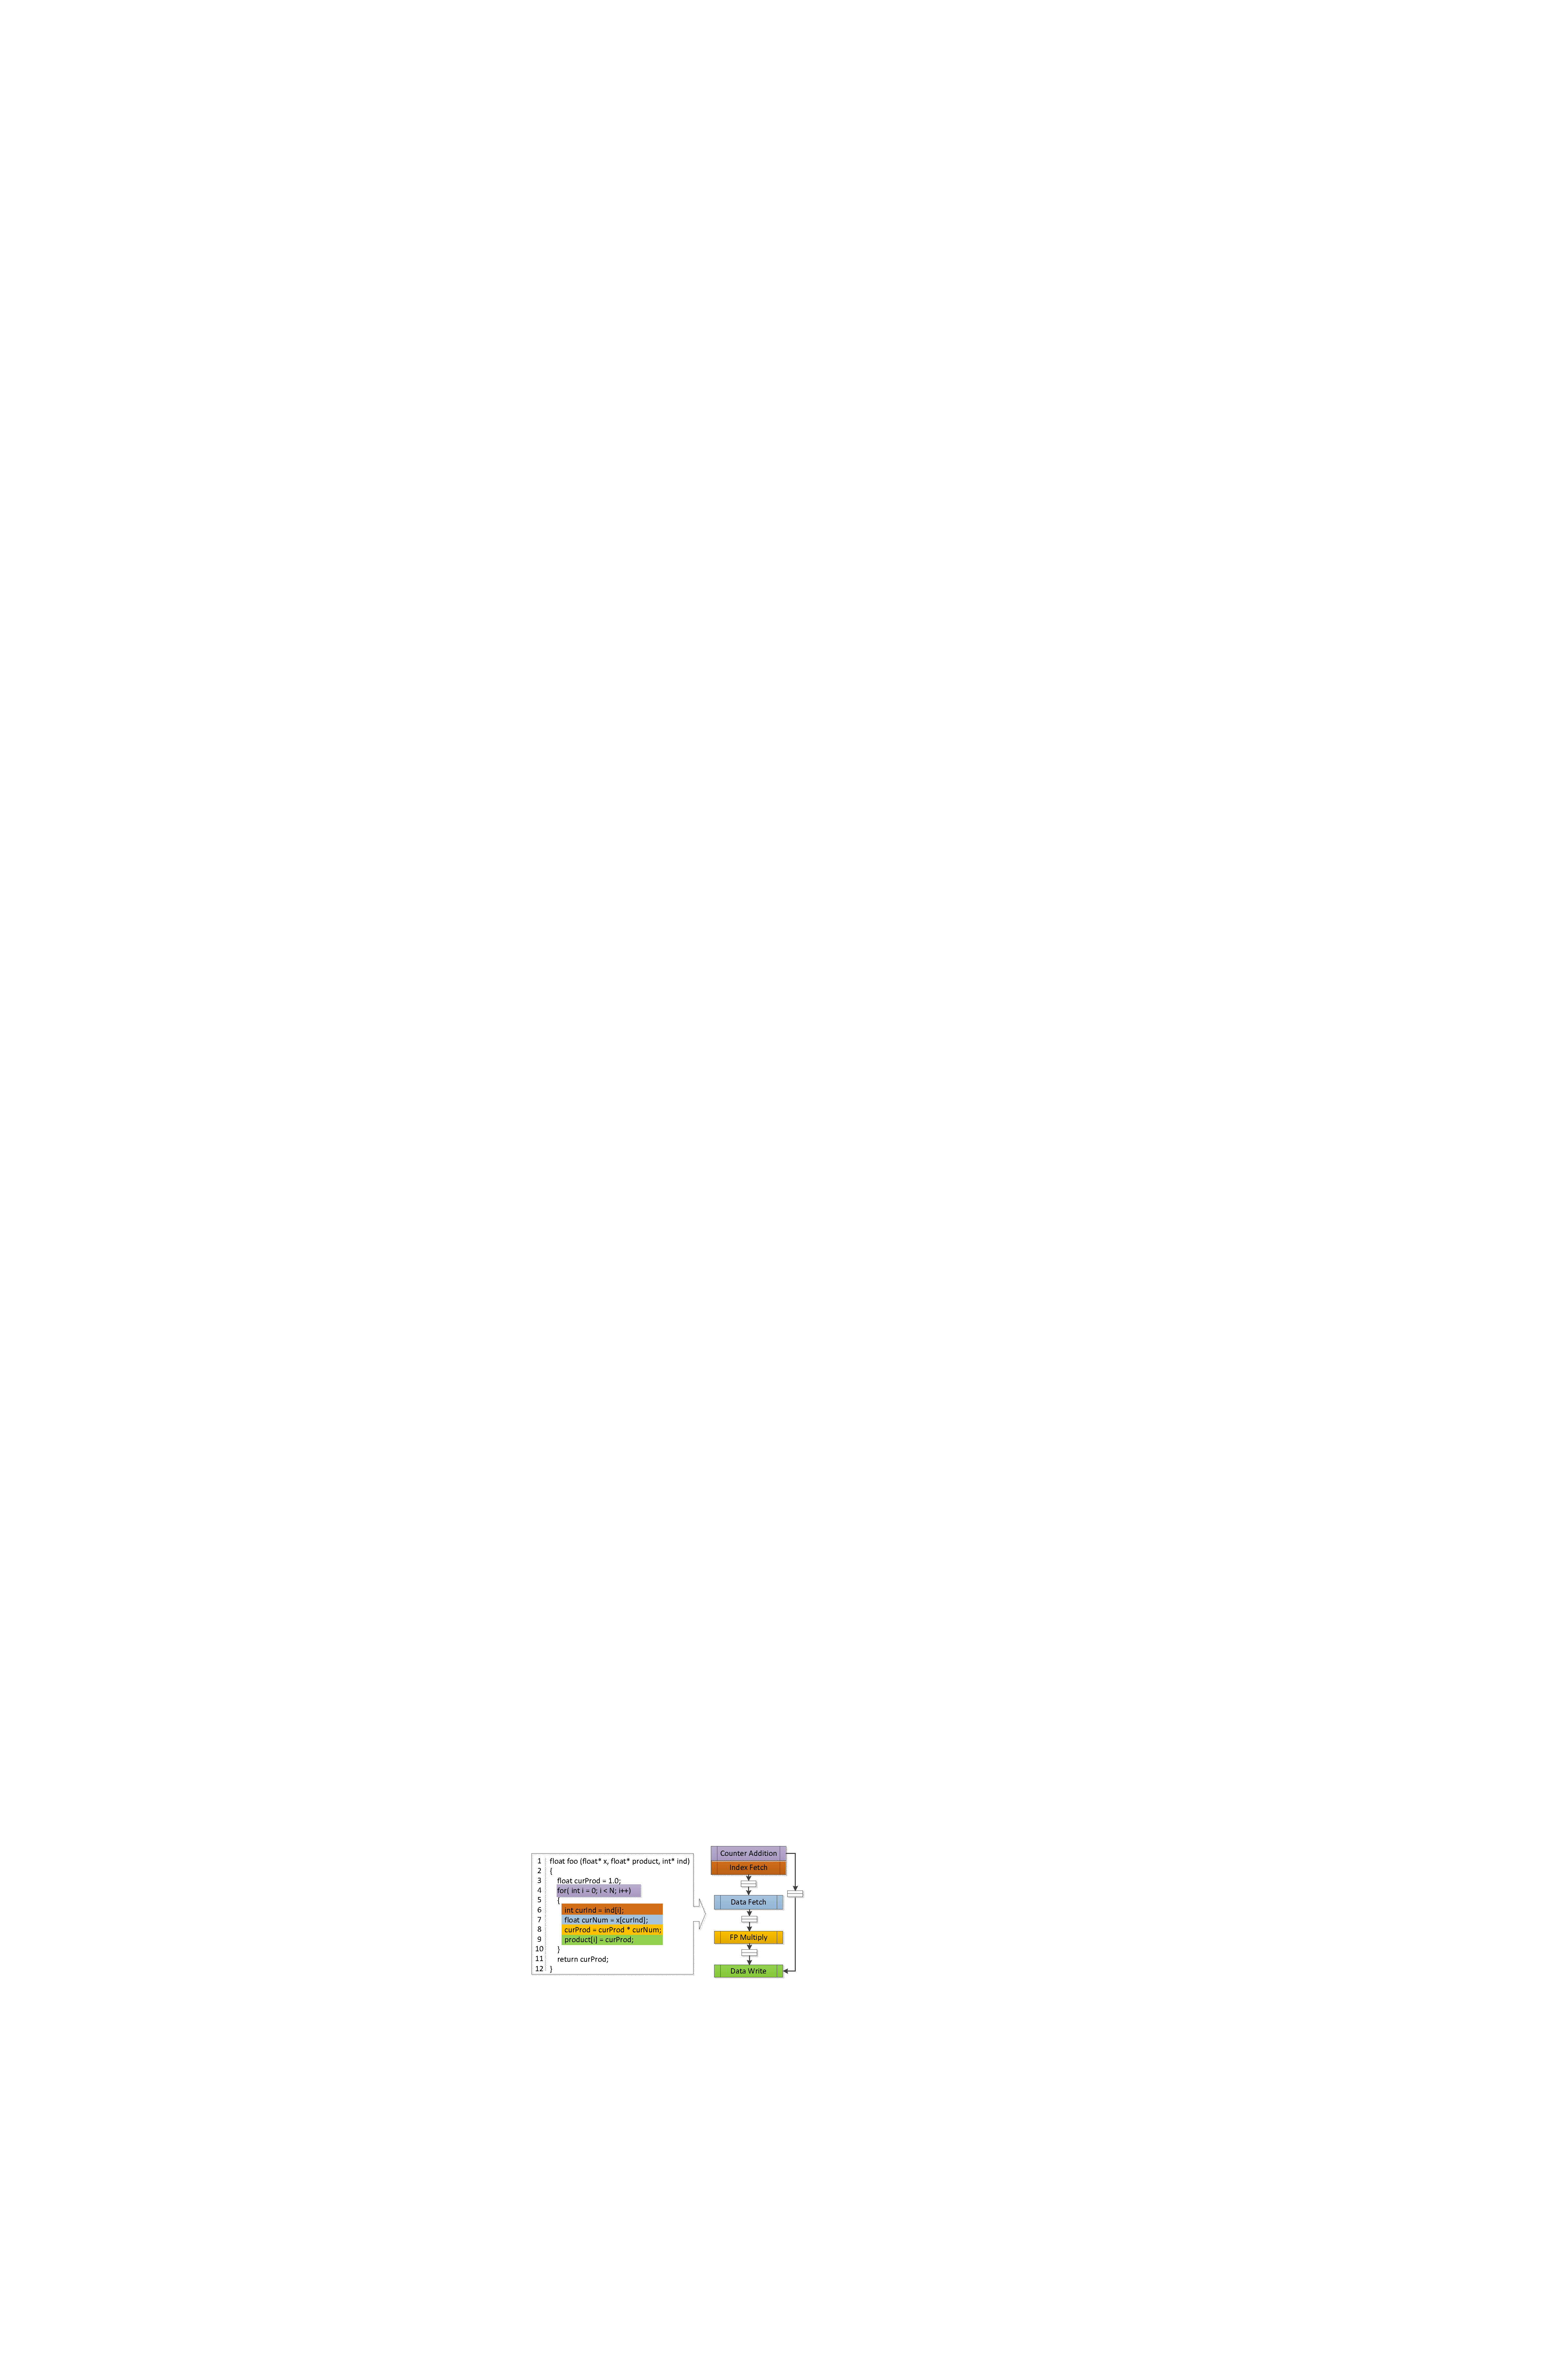
\includegraphics[width=0.6\linewidth]{chap3fig/motExample.pdf}
\caption{Converting a Simple Function to Decoupled Computational Pipeline
\label{fig:motivating}}
\end{center}
\end{figure}

\section{A Motivating Example}
\label{motex}
Shown in figure~\ref{fig:motivating} is a simple example where separating a software kernel into multiple decoupled stages can improve the overall performance. As the shown function
is pushed through the conventional HLS flow, opportunities for parallelization are
discovered and a static schedule can be generated. The loop counter addition and the loading of $curInd$ can happen simultaneously, and the next iteration of the  loop
can start before the current iteration finishes. Meanwhile, because the floating-point
multiply always uses its result from the previous iteration, the shortest interval with which we can start a new iteration is limited by the latency
of the multiplier. The execution schedule of this function is shown in figure~\ref{fig:sche}(a).

This execution schedule, unfortunately, assumes the best case latency for all the memory accesses. Since the computation kernel is turned into a monolithic accelerator,
the centralized controller would have to stall the entire compute engine when long latency off-chip communication operations are occurring. This is less of an issue when the memory access patterns are known \textit{a priori}, such that the data can be moved on-chip before
it is needed, or if the data set is small enough to be entirely buffered on the FPGA.
However, in this example, just like in many interesting algorithms, the data access depends on the result of computation and the memory footprint requires the use of off-chip storage. Figure~\ref{fig:sche}(b) shows the execution of the generated hardware module
in the presence of cache miss stalls. Note how the slowdown reflects the combination
of all cache miss latencies. This does not have to be the case though, since there are
parts of the computation graph whose progress does not need the memory data to be immediately available. These sections should be able to move forward. This extra bit of
freedom in the execution schedule can potentially have a significant effect.

In this example, it is possible to decouple the execution of the floating point multiply and the data accesses from each other. Without a unified schedule, one load operator can keep requesting new data while the other one waits for previous requests to be responded by off-chip storage, and the floating point multiplier works through
previously fetched data. This is achieved by having one module responsible for each
of the memory accesses and the multiplication, as shown in figure~\ref{fig:motivating}.
The FIFOs allow for the communication between these modules, while buffering the data
already produced but not yet consumed. Over a long period of time, the stalls introduced by the memory accesses are shadowed by the long latency of the floating point multiplier, who is always supplied with the backlog of data in the FIFO when
cache misses occur. As long as the overall bandwidth provided by the memory subsystem
satisfies the need of the computation, the latency of the memory accesses can be
tolerated. 

Figure~\ref{fig:sche}(c) shows the execution schedule when the decoupled pipeline is used. The latencies through the FIFOs are not taken into consideration here, e.g. FP multiply starts immediately after completion of $curNum$ load, but their effect
should be minimal when amortized over a large number of iterations. 


\begin{figure}[htp]
\begin{center}
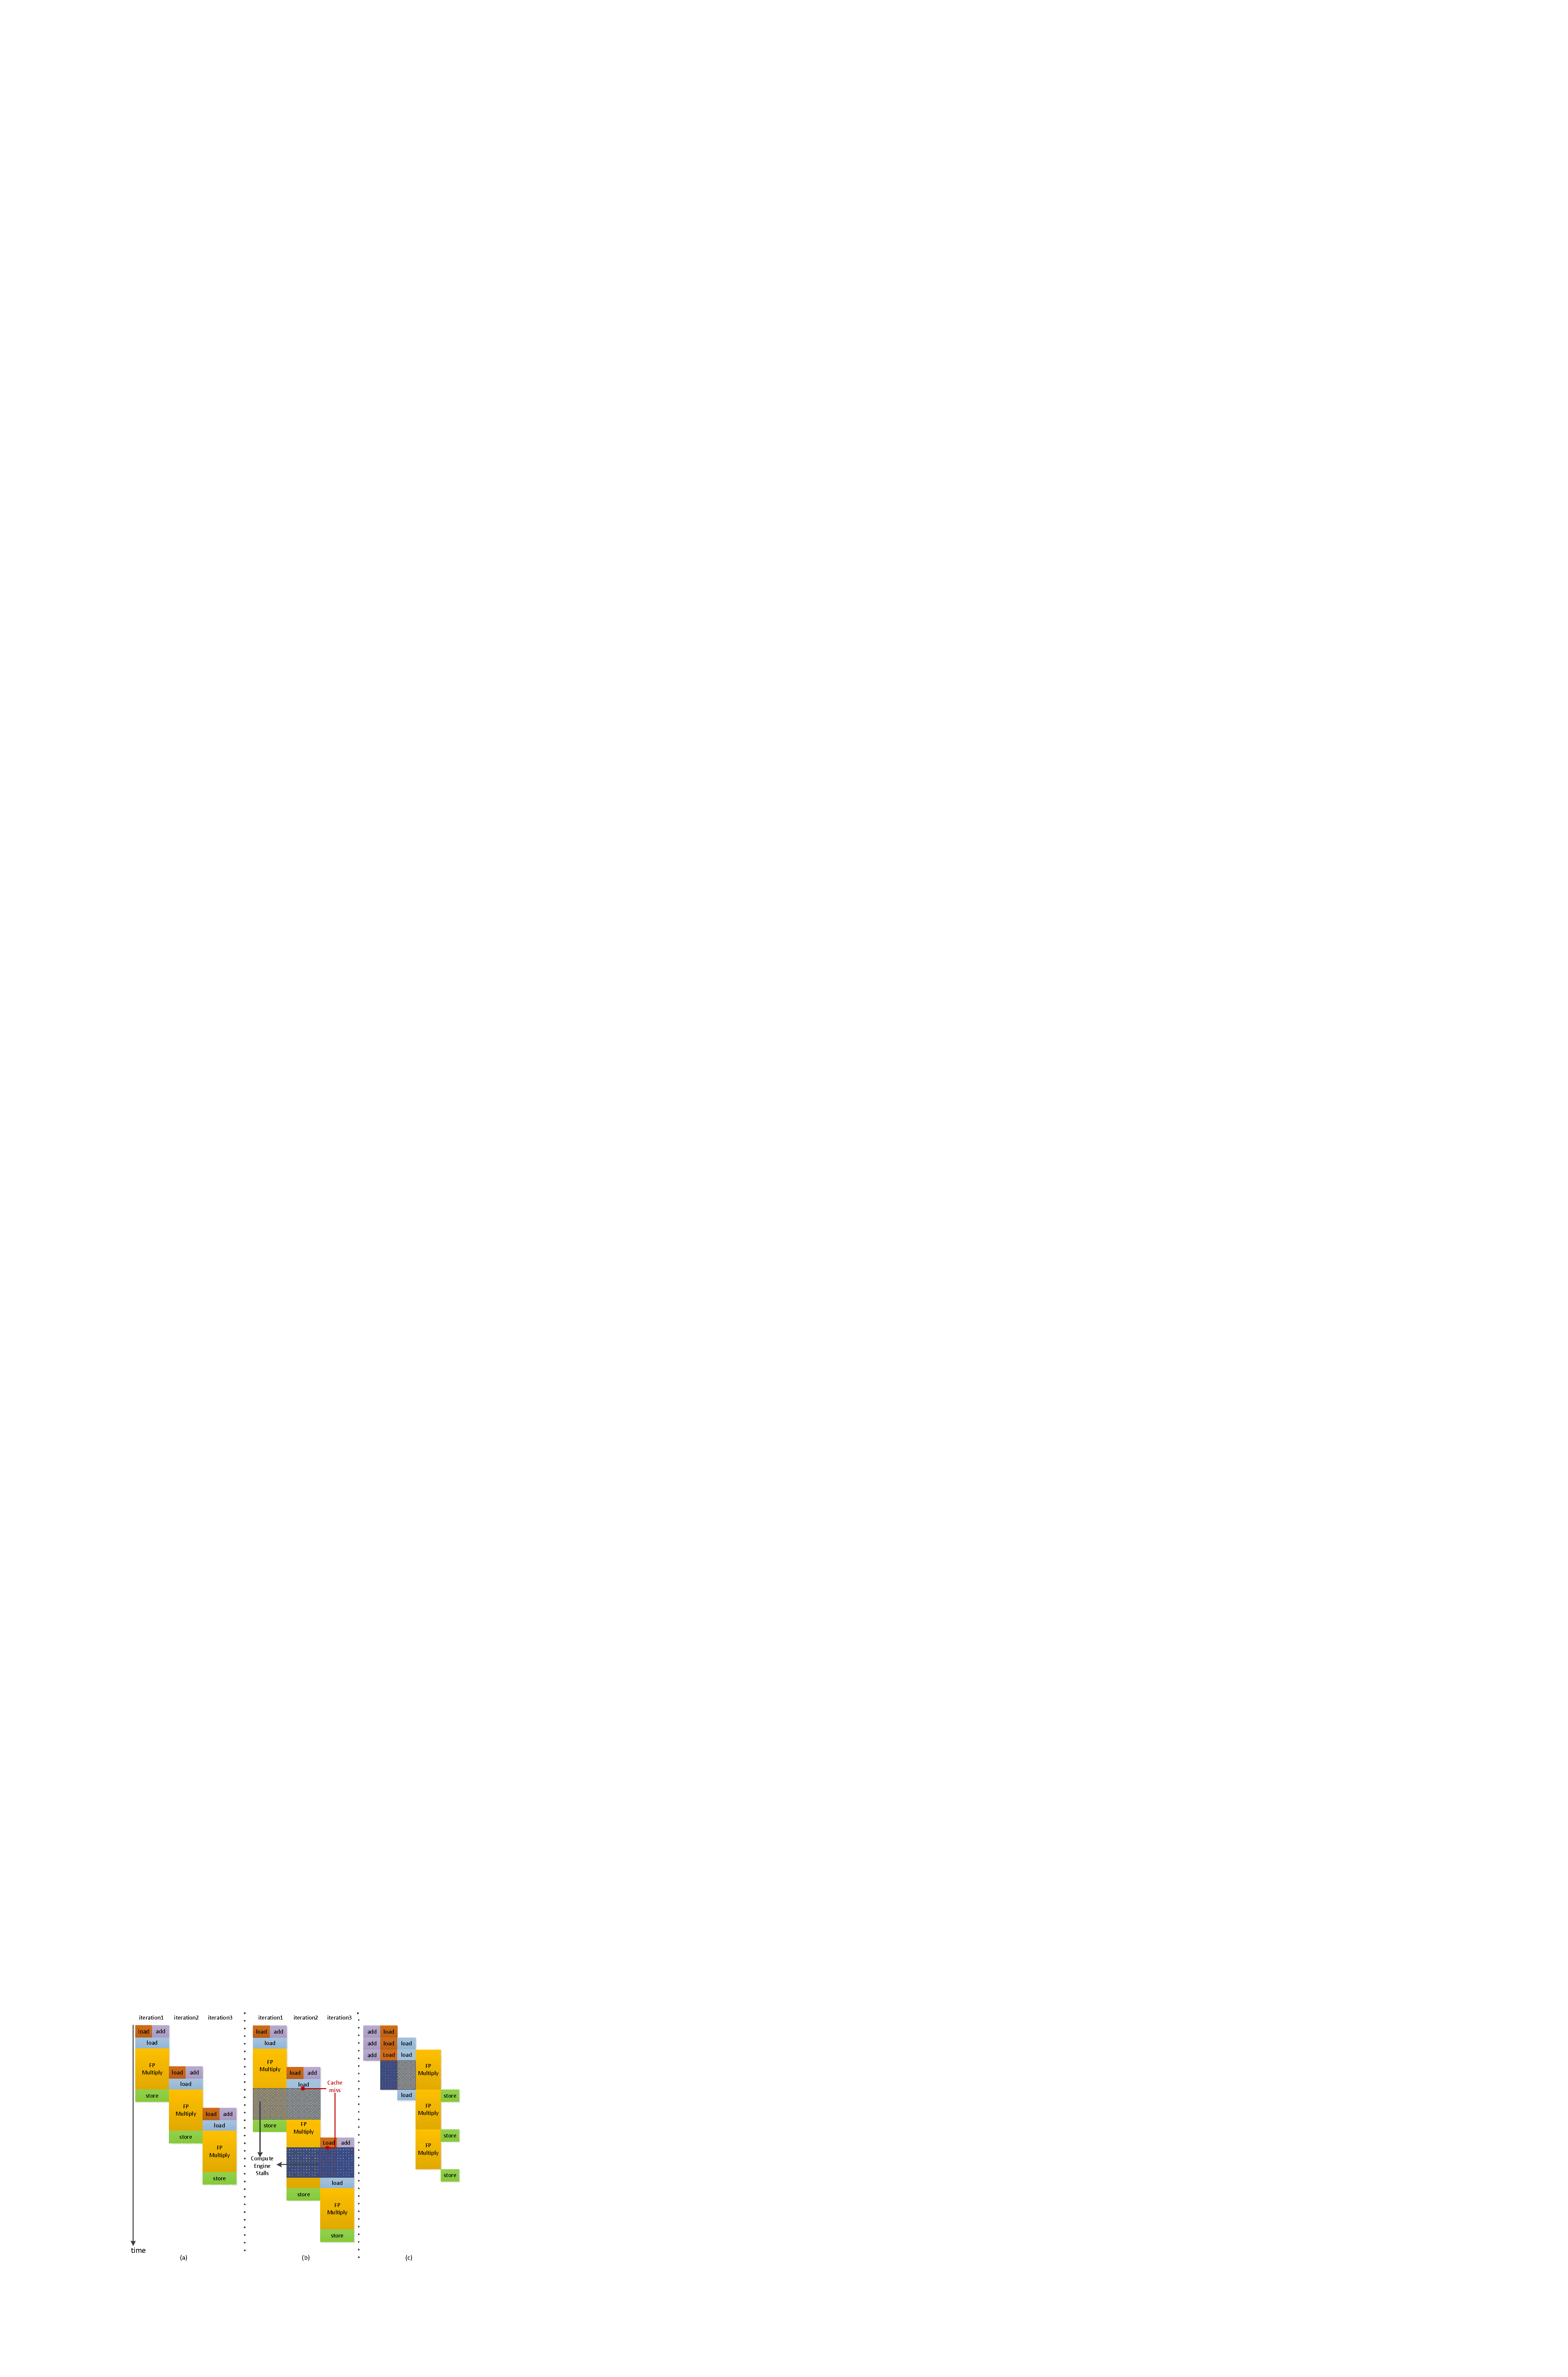
\includegraphics[width=1.0\linewidth]{chap3fig/schedules.pdf}
\caption{(a) Static schedule produced by HLS (b) Actual Execution with Cache Misses (c) Execution of Decoupled Computational Pipeline 
\label{fig:sche}}
\end{center}
\end{figure}

\section{Partitioning the Instructions}
\label{sec:partins}
To generate modules who are running out of sync from each other, the original
control data flow graph (CDFG) needs to be partitioned into multiple sets.
Each set is to be converted to a self-contained function and synthesized to
a stage in our pipeline.
To maximize the performance of the resulted implementation, a few factors
should be considered during our partitioning process. 
First, circular dependencies between
nodes of the innermost loop need to be contained within each set. These strongly
connected components (SCCs) in CDFG are associated with
loop carried dependencies, and are the limiting factors for how
aggressively loop iterations can be overlapped. The initiation
interval (II) of loops are dictated by the latency of these cycles.
As the communication channels will always add latency,
having parts of an SCC in CDFG scattered across multiple
stages would increase the II of the iterations, which are now
executed in a distributed manner. 
Secondly, as we have demonstrated in section~\ref{motex}, with memory operations separated
from dependency cycles involving long latency compute, we
can have cache misses completely hidden by the slow rate
of data consumption.
Thirdly, to
localize the effects of stalls introduced by cache misses, the
number of memory operations in each set should be
minimized, especially when they address different parts of the
memory space.



 


%\begin{figure}[htp]
%\begin{center}
\begin{algorithm}[t]
  \caption{Instruction Partitioning}\label{algo1}
  \begin{algorithmic}[1]
  \Procedure{PartitionCDFG}{G}%\Comment{G: CDFG of loop nests}
    \LineComment{SCCs of instructions formed with data/control/memory dependency edges}
    \State SCCs $\gets$ allStronglyConnComps(G)
  \State DAG $\gets$ collapse(SCCs,G)
  \State topoSortedNodes $\gets$ topologicalSort(DAG)
  \State longSCCs $\gets$ getSCCWithLongOp(SCCs)
  \State memNodes $\gets$ findLdStNodes(G)
  \State memLongSCC $\gets$ LongSCCs $\cup$ memNodes
  \State allSets $\gets \{\}$
  \State curSet $\gets \{\}$
  \While{topoSortedNodes $\ne \emptyset$}
     \State curNode $\gets$ topoSortedNodes.pop()
     \State curSet $\gets$ curSet $\cup$ curNode
    
     \If{curNode $\in$ memLongSCC}
     %\If{$curSubG \cap MemLongSCC \ne \emptyset$}
    \State allSets $\gets$ allSets $\cup$ curSet
    \State curSet $\gets$ \{\}
     %\EndIf
     \EndIf

     %\State $curSubG \gets curSubG \cup curNode$
     
  \EndWhile
  \State \Return allSets 
  %\State $OtherNodes = G - SCCs - MemNodes$
  %\State $SNodes\gets collapseSCC(G, SCCs)$
    %\State $i\gets 0$
    %\foreach{$r\not=0$}\Comment{We have the answer if r is 0}
  %\State $SGs\gets ClusterWithSeed(SCCs, MemNodes)$
  %\State $MGs\gets ClusterWithSeed(MemNodes, MemLongSCC)$
  %\State $OGs\gets ClusterWithSeed(OtherNodes, MemLongSCC)$
  %\State \Return $SGs \cup MGs \cup OGs$
  %\While{$SCCs \ne \emptyset$}
  %  \State $curSubG\gets \{\}$
  %  \State $curSCC\gets SCCs.pop()$
  %  \State $DFSCluster(curSCC,curSubG,MemNodes)$
  %  \State $Subgraphs\gets Subgraphs \cup curSubG$
  %\EndWhile
  %\While{$MemNodes \ne \emptyset$}
  %  \State $curSubG\gets \{\}$
  %  \State $curMem\gets MemNodes.pop()$
  %  \State $MemLongSCC\gets LongSCCs \cup MemNodes$
    %  \State $DFSCluster(curMem,curSubG, MemLongSCC)$
  %  \State $Subgraphs\gets Subgraphs \cup curSubG$
  %\EndWhile
  %\While{$OtherNodes \ne \emptyset$}
  %  \State $curSubG\gets \{\}$
  %  \State $curN\gets OtherNodes.pop()$
  %  \State $MemLongSCC\gets LongSCCs \cup MemNodes$
    %  \State $DFSCluster(curN,curSubG, MemLongSCC)$
  %  \State $Subgraphs\gets Subgraphs \cup curSubG$
  %\EndWhile
  %now do the otherNodes
  
    %\EndWhile\label{euclidendwhile}
    \EndProcedure
  %\Procedure{ClusterWithSeed} {$seeds$, $excludeSet$}
  %\State $subgraphs\gets \{\}$
  %\While{$seeds \ne \emptyset$}
    %\State $curSubG\gets \{\}$
    %\State $curN\gets seeds.pop()$
    %\State $DFSCluster(curN,curSubG, excludeSet)$
    %\State $subgraphs\gets subgraphs \cup curSubG$
  %\EndWhile
  
  %\State \Return $subgraphs$
  %\EndProcedure
  
  %\Procedure{DFSCluster} {$curN$, $curG$, $excludeSet$}
  %\If{$curN.isCovered()$}
  % \Return
  %\EndIf
  
  %\If{$curN \in excludeSet$}
  % \If{$curG \cap excludeSet \ne \emptyset$}
  %   \Return
  % \EndIf
  %\EndIf
  %\State $curG \gets curG \cup curN$
  %\State $curN.setCovered(true)$
  %\State $nextNodes\gets getDependents(curNode, DAG)$
  %\While{$nextNodes \ne \emptyset$}
  % \State $nextNode \gets nextNodes.pop()$
  % \State $DFSCluster(nextNode, curG, excludeSet)$
  %\EndWhile
  %\EndProcedure
  \end{algorithmic}
\end{algorithm}

\subsection{Partitioning Algorithm}
The first factor was one of the observations made 
in~\cite{dswp}, where sequential programs were converted into multithreaded
codes running on multicore processors. Their algorithm
finds strongly connected components (SCCs) in the
original dataflow graph, collapses them into nodes and then
heuristically partitions the resulted directed acyclic graph
(DAG) into threads with balanced load. In our flow, the search
for SCCs is also necessary and its outcome is used for the
ensuing partitioning, which centers upon memory operations.
In Algorithm~\ref{algo1}, the steps taken to perform the partitioning are detailed.
The SCCs are collapsed into new nodes, which together with the original nodes in the CDFG, are topologically
sorted. The obtained directed acyclic graph is traversed and a new set is created whenever a memory operation
or an SCC with long latency computation
is encountered. Here, long latency operations are those which cannot be completed within
one clock cycle, and
their categorization ultimately depends on the target frequency
of the final implementation on the FPGA. Currently, we
leverage Xilinx’s Vivado HLS to generate latency estimate for
various compute operations. With a target clock frequency of
150MHz, for instance, floating point multiply takes four clock
cycles while a 32 bit integer addition can be completed within
a cycle. As Vivado HLS is eventually used as the backend for
our HDL generation, it provides accurate annotations for our
flow.
\begin{figure}[htp]
\begin{center}
\includegraphics[width=0.9\linewidth]{chap3fig/order.pdf}
\caption{Three Types of Memory Dependencies
\label{fig:memorder}}
\end{center}
\end{figure}
 
\subsection{Preserving Memory Dependency }
\label{subsec:pmd}
The semantics of the input high level language often create
dependencies implicitly carried by memory accesses.
Given two statements in a program, Bernstein's conditions~\cite{4038883} described when
they are independent and can be executed in parallel or out of order.
If two memory operations access the same location and one of them is a store, their order in the original program execution must be preserved. More specifically, three types of dependencies need to be observed:
\begin{itemize}
    \item Read-after-write (RAW) -- When the same memory location is written by one statement and read by the other, there is a dataflow dependence between them (figure~\ref{fig:memorder}a). Performing them out of order results in the outdated operand to be used by the consumer statement. 
    
    \item Write-after-read (WAR) -- When a memory location is read by the first statement and subsequently written by the second, there is an anti-dependence between them (figure~\ref{fig:memorder}b). Performing them out of order overwrites
    the correct operand prematurely. 
    \item Write-after-write (WAW) -- When both statements write to the same location, there is an output dependence between them (figure~\ref{fig:memorder}c). Reordering the two
    writes exposes the wrong value to the subsequent reads.
\end{itemize}
 For every pair of operations whose ordering needs to be preserved, a special dependency edge is added between them. Since the generation of the sets is performed around strongly connected components in the original dataflow, it is important to avoid adding unnecessary memory dependency edges. To achieve this, our flow currently relies on alias analysis to perform partitioning of the memory space. Accesses to disjoint memory regions can be safely reordered. When the source code contains pointer arithmetic or irregular memory accesses, compile time alias analysis may produce overly conservative results, in which case user annotations can be used to provide hints to the tool, similar to~\cite{manycache}. This partitioning of memory space naturally leads to creation of multiple data access interfaces, whose interactions with the memory subsystem can be customized, as will be elaborated in section~\ref{sec:optmem}.  



Under certain circumstances, we do not want to directly add edges between memory operations
as they hinder the CDFG partitioning. For the example in figure~\ref{fig:barrier}, during the execution of one outer loop iteration, the set of memory addresses accessed by the the load does not intersect
with that of the store instruction. However, across different outer loop iterations, these
two instructions can accesses the same locations. 
We can conservatively make them dependent
on each other, but this creates an SCC that ultimately prevents any partitioning, as can be
seen in the figure.



%become the performance bottleneck. 
Alternatively, a memory barrier can be inserted after the completion of 
each outer loop iteration. 
%To implement the barrier in the pipeline, the stage containing
%the semantically earlier instruction sends tokens to stages who contain the %successor instructions. In figure~\ref{fig:barrier}, 
To implement the barrier in the pipeline, the stage in charges of the last 
memory operation before the barrier broadcasts ``barrier" tokens to pipeline stages who contain memory operations following the barrier. 
Eventually during the RTL generation, the local schedule of instructions also needs to be constrained such that the sender of the barrier tokens is not reordered to before its memory accessing predecessors, while the receivers of barrier tokens must execute before their memory accessing successors in the original program order as well.
In figure~\ref{fig:barrier}, the store operation (A[i][j] = tmp) is followed by the sender of the barrier token, whereas the load operation (tmp = A[i-1][j]) in the other pipeline stage waits for the reception of barrier token for the previous outer loop iteration.


The insertion of the sender/receiver of the barrier happens after the instruction partitioning. Depending on if a partition is the sender or receiver of the token,
an extra store/load operation is introduced into the set of instructions, associated
with the basic block where the barrier occurs.


\begin{figure}[htp]
\begin{center}
\includegraphics[width=1.0\linewidth]{chap3fig/barrier.pdf}
\caption{Barrier for Enforcing Order of Memory Accesses
\label{fig:barrier}}
\end{center}
\end{figure}

\subsection{Control Dependency Edges}
Another source of edges in our CDFG -- control dependency, also warrants some 
discussion. The simplest way to add the control dependency edges is to have
every instruction dependent on the control transfer instructions of the immediate
predecessors of its container basic blocks. For a loop nest, this will necessarily
create a single SCC with all the branch instructions of the basic blocks within the loop nest. Essentially, a control flow ``backbone" is generated and the branch
tag tokens will need to be sent to all other modules whose instructions are predicated on these branches. The pipeline thus generated, while valid, may
have higher communication channel count and less opportunities for optimization
within each module, which will be elaborated more in section~\ref{sscf}. We thus
perform a more aggressive predication/control edge insertion by looking for the
earliest branch outcome which necessarily leads to the execution of an instruction. Given an instruction $i$ and its container basic block $bb$, our
flow looks for the nearest set of basic blocks $BB'$ who are not properly post-dominated by $bb$,
and insert the dependency edge between the branch instructions ending each member of $BB'$ and $i$.




\begin{comment}
Also, to ensure the barrier tokens are sent out only after the completion of preceding 
memory operations, which are often signaled by special \textit{RESP} lines,  a special module is created to monitor and coordinate the transmission of the tokens. Its structure
is shown~\ref{}, only when 
As we are trying to ensure the semantically later instructions
do not get ahead of their predecessors, the barrier is implemented by having the stage containing the later instruction sending tokens to an earlier stage in the pipeline. As the local schedule 
\end{comment}

%There is a possibility that the load instruction of an later outer loop iteration occurring 

%in the inner most loop can be separated as the memory dependency edges do not form a circle. However, 


\section{Construction of Pipeline of Subgraphs}
\label{sec:consp}


With instructions partitioned into disjoint sets, the flow then
reconstruct subgraphs from these sets of instructions. Each subgraph
contains a subset of the original control flow/basic blocks and 
will later be synthesized as a self-contained function. The reconstruction process involves adding relevant basic blocks according to the
association of the instructions with the current set.
\begin{itemize}
    \item For every instruction $i$  in the current set, recreate
    its container basic block if it's not already in the current subgraph.
    \item For every instruction $j$  $i$ depends on, 
    recreate its container basic block if it's not already
    in the current subgraph.
    \item If $j$ is associated with another subgraph, a ``pop" function call
    is added locally as a placeholder in its container basic block.
    %a load operation
    %is created locally as a placeholder in its container basic block.
    \item If $i$ is producing operands for instructions assigned to 
    other sets,  a ``push" function call is inserted after $i$.
    %a store operation is inserted after $i$.
\end{itemize}
The set of recreated basic blocks $B$ are thus associated with either the instructions
assigned to the subgraph, or the placeholder function call supplying them with operands. To mirror the relevant execution path in the original program, a few more steps need to be taken.
\begin{itemize}
    \item In the control flow of the original program, find the nearest common dominator $d$ of all the recreated basic blocks $B$, and add $d$ to $B$. It will be the entry block of our
    control flow in this subgraph.
    
    \item Find all the paths $P$ from $d$ to $b \in B$, add all the 
    basic blocks in each $p \in P$ to $B$.
    \item From each $b \in B$, find the paths $P_b$ to every $b' \in B$ without passing through $d$. Add all the basic blocks in each $p_b \in P_b$ to $B$. \item Create the branching instructions at the end of each $b \in B$. If the branching instruction was already assigned to the current subgraph, nothing needs to be done, otherwise a load operation is created to accept
    a branch target token from another subgraph, and then the actual branching is performed according to the received token. 
    \item If $d$ was inside a loop in the original control flow, any branch out of the set $B$ is redirected to $d$. Otherwise, any branch out of the set $B$ terminates the execution of this subgraph.
\end{itemize}


\begin{figure}[htp]
\begin{center}
\includegraphics[width=1.0\linewidth]{chap3fig/totalflow.pdf}
\caption{(a) The Motivating Example in Single Static Assignment Form (b) Partitioning of Instructions (c) Pipeline of Reconstructed Subgraphs
\label{fig:totalFlow}}
\end{center}
\end{figure}

In the control flow graph of the original program, the set of paths whose starting points and end points both fall in $B$ can be divided into
two groups. Some of these paths never reach basic blocks outside of $B$, and the rest go out of $B$ and then come back into $B$ via $d$. 
The first group
is completely contained within our subgraph.  If there is any path in the second group, then $d$ must be inside a loop, in which case we have effectively enclose the subgraph with a \textit{while(true)} loop and the execution of the part
of the path within the subgraph
will be repetitively activated by the availability of the proper tokens.

The insertion of %load and store 
``pop" and ``push"
operations is necessitated by various
dependencies between the generated subgraphs. Other than data and control (branch) tokens we have mentioned, special tokens are also sent when ordering
of memory accesses needs to be enforced. Each of the inserted operations corresponds to a hardware queue between the decoupled modules, the flow of
tokens ensures the execution path are synchronized across different subgraphs
and the right operands are supplied for computations distributed across the
pipeline.
\begin{comment}
The dependencies between the generated subgraphs necessitate the insertion of communication primitives. In our case, these correspond to the load and store operations to/from a hardware queue between the decoupled modules.  
Other than the explicit data flows, control dependencies are also communicated using branch target tags, such that the local branch operations can synchronize across different subgraphs. Lastly, in the case where ordering of memory accesses needs to be enforced, special tokens are sent between modules.
\end{comment}
Eventually, in the hardware module synthesized from each subgraph, these ``pop" and ``push" operations %loads and stores 
are blocking, as they operate on standard FIFO interfaces. Flow control between different pipeline stages are thus naturally introduced. The execution of the entire processing pipeline is completed when all modules are idling waiting for inputs and all hardware queues are empty. The runtime behavior of this pipeline thus resembles a streaming processing engine, with uncertainties introduced by memory access nodes smoothed out by FIFOs.



The implementation of our partitioning algorithm and the insertion of the communication primitives leverage the LLVM infrastructure~\cite{llvmflow}. The LLVM front end converts the instructions in the original program to the single static assignment (SSA) form, which makes it easy to track dependencies and thus facilitates all the steps in our algorithm. Figure~\ref{fig:totalFlow} shows the SSA form
of our example function and how the instruction partitioning and subgraph reconstruction can be easily performed given the explicit representation of
dependencies. For better readability, we have converted the LLVM SSA intermediate representation (IR) to a less verbose, C-like version. Operators not available in C are explained in the figure. The inserted communication primitives are highlighted,
the parameters to these ``push" and ``pop" invocations include the names of the associated queues and the data variables.
%To highlight
%the inserted communication primitives, we show them as ``push" and ``pop" function %calls taking in the queue name and the data variable name as the parameters.  


It is worth noting that transformations in LLVM framework are organized as ``passes". Well-formed LLVM IR should be fed to and obtained from each of these passes. For our flow, a single loop-containing LLVM function is broken into multiple LLVM functions who communicate with each other and collectively perform the same computation as the original subroutine. To ensure each of the generated
 LLVM functions is well-formed, pointers are added to its argument list to represent the FIFO interfaces the token loads/stores act upon. The original subroutine, on the other hand, has all its computation replaced by invocation of these generated functions,in addition to allocation of memory spaces as placeholders for communication channels. This is illustrated in figure~\ref{}.
 As our pipeline is represented in proper LLVM IR, additional optimization or analysis passes can be applied to it.
 
\begin{comment} 
In figure~\ref{fig:totalFlow}, the conversion process from the example function (in SSA form) to the final pipeline of subgraphs is illustrated. For better readability, we have converted the LLVM intermediate representation (IR) to a less verbose, C-like version. Operators not available in C are explained in the figure.
To highlight
the inserted communication primitives, we show them as ``push" and ``pop" function calls taking in the queue name and the data variable name as the parameters. The execution of the entire processing pipeline is completed when all modules are idling waiting for inputs and all hardware queues are empty. The runtime behavior of this pipeline thus resembles a streaming processing engine, with uncertainties introduced by memory access nodes smoothed out by FIFOs.
\end{comment}









%As shown in figure 2, subgraphs whose first instruction reads value off a FIFO should be placed in an infinite loop to ensure it is repeated the right number of times, which is especially important if the subgraph is strictly within a loop. The execution of the entire processing pipeline is completed when all modules are idling waiting for inputs and all hardware queues are empty. The runtime behavior of this pipeline thus resembles a streaming processing engine, with uncertainties introduced by memory access nodes smoothed out by FIFOs.

% Figure 2 illustrates the result of clustering on our earlier example. Each of the generated subgraphs (SGs) corresponds to a decoupled stage in figure 1. For better readability, we have converted the LLVM intermediate representation to a less verbose, C-like version. Operators not available in C are explained in the figure.
%After the partitioning, the edges spanning two stages will be converted to communication channels 
%for data/control tokens 
%to be passed between them. From each stage's perspective, these are just normal load/store operations
%from/to special pointers corresponding to communication interfaces. During the actual hardware
%generation, FIFOs will be instantiated and connected. 




\begin{comment}
Conceptually, a
topological sort is performed on the DAG formed after the
SCCs are collapsed into single nodes. In the linear array thus
obtained, we find memory operations and SCCs with long
latency compute operations, which are tagged as “terminals”
for our clustering process. The algorithm then traverses the
array, starting a new cluster every time a “terminal” is added.
The detailed steps involved are shown in Algorithm 1.
\end{comment}

% mention compaan compiler and affine loop

\section{Optimization of Computational Pipeline}
With an initial implementation of the computational pipeline, there are a few simple optimizations we can perform to improve its overall efficiency. 

\subsection{Simplification of Subgraph Control Flow}
\label{sscf}
As mentioned in section~\ref{sec:consp}, we generate the control flow of a subgraph by
recreating basic blocks to form a self-contained function, in which every path from
any member basic block to any other ones are covered. This approach sometimes introduces 
basic blocks whose only purpose is to have the execution path going through them, instead
of doing any computing. Depending on the actual structure of the control flow graph, some
of these blocks can be completely removed with proper redirection of branches. 

To perform this simplification, we want to eliminate those basic blocks who do not
perform any computation/communication, and are not divergent points in the control flow.
More specifically, let the set of all basic blocks be $BB_{all}$, the set of basic blocks containing receiver load instructions (other than receiver of branch tags) be $BB_{comm}$ and the set of basic blocks performing some computation
be $BB_{comp}$, algorithm~\ref{algo2} outlines the steps for this optimization.
\begin{algorithm}[t]
  \caption{Control Flow Simplification}\label{algo2}
  \begin{algorithmic}[1]
  \Procedure{SimplifyCFG}{}%\Comment{G: CDFG of loop nests}
    \State keepers $\gets \{\} $
    \State keeperQueue $\gets BB_{comm} \cup BB_{comp}$
  \While{keeperQueue $\ne \emptyset$}
     \State curKeeper $\gets$ keeperQueue.pop()
     \State keepers $\gets$ keepers $\cup$ curKeeper
     \State allPredecessors $\gets$ getPredecessors(curKeeper)
     
     \ForAll{ curPredecessor $\in$ allPredecessors}
     \LineComment{look for divergent points from predecessors}
     \State backwardDFS(curKeeper, curKeeper, curPredecessor, keeperQueue)
     \EndFor
  \EndWhile
  
  \EndProcedure

  \Procedure{backwardDFS}{curKeeper, prevStep, curPredecessor, keeperQueue}
  \If{curPredecessor $\notin BB_{all}$}
  \Return
  \EndIf
  \If{!curKeeper.postDominate(curPredecessor) }
  \State keeperQueue.push\_back(curPredecessor)
  \State remapBranch(curPredecessor, prevStep, curKeeper)
  \State curKeeper $\gets$ curPredecessor
  \EndIf
  \State allPredecessors $\gets$ getPredecessors(curPredecessor)
     \ForAll{ nextPredecessor $\in$ allPredecessors}
     \State backwardDFS(curKeeper, curPredecessor, nextPredecessor, keeperQueue)
     \EndFor 
  \EndProcedure
  \Procedure{remapBranch}{predecessor, prevTarget, realTarget }
  \State branchInst = predecessor.getBranchInst()
  \State branchDstBBs = branchInst.getAllSuccessors()
  \State branchDstInd $\gets 0$
     \ForAll{curDstBB $\in$ branchDstBBs}
     \If{curDstBB = prevTarget}
     
     \LineComment{make the destination pointed to by branchDstInd $realTarget$}
     \State predecessor.setSuccessor(branchDstInd, realTarget) 
     \EndIf
     \State branchDstInd $\gets$ branchDstInd + 1
     \EndFor 
  \EndProcedure
  \end{algorithmic}
\end{algorithm}

Our algorithm looks for basic blocks who may branch out of the subgraph, or can branch (directly
or indirectly)
to more than one members among $BB_{comm}$ and  $BB_{comp}$, and 
change their branches' destinations while deleting unnecessary basic blocks. As illustrated in figure~\ref{fig:cfsim}, this optimization reduces the number of branch tag tokens to be transmitted
between different subgraphs and thus the number of communication channels
needed. It also reduces each subgraph's complexity, making the generated hardware smaller and faster. 
In the simplified CFG in figure~\ref{fig:cfsim}, the original outer loop becomes
an inner loop, thus can be pipelined independent from the inner loop in the
other subgraph.

\begin{figure}[htp]
\begin{center}
\includegraphics[width=1.0\linewidth]{chap3fig/cfgRecSim.pdf}
\caption{Subgraph Reconstruction and Simplification 
\label{fig:cfsim}}
\end{center}
\end{figure}

\subsection{Duplication over Communication}
\label{dupvscomm}
An apparent overhead our flow introduces comes from the mechanisms added
for different subgraphs to communicate with each other. In hardware accelerators,
these are manifested as resource overhead in implementing the extra load and
store operations in each subgraph and more importantly, the FIFOs
between different subgraphs. Table~\ref{tab:fifoResource} shows the
resource usage for some FIFO configurations implemented on our experiment platforms. Given how even a minimal depth FIFO 
can use a non-trivial amount of FPGA, it is often beneficial to duplicate some of the computations to multiple subgraphs.
For each subgraph, each of the nodes preceding it in the DAG used for
instruction partitioning may be duplicated. By copying some of
these nodes into the subgraph, the edges cut by the subgraph boundaries
also change and there can be an overall saving. 
%Figure~\ref{fig:gc} shows how we can formulate this problem as in graph representation. The initial cut, for instance, cut through the edge between
%node $D$ and $subG$, which carries a cost $W_H$. If the combined cost of node $D$ and edge $AD$ ($W_L$) is lower than $W_H$, we can duplicate 
In this graph cut problem (figure~\ref{fig:gc}), we want to minimize the sum of the cost of the cut edges
and the duplicated nodes.  Since we are duplicating instead
of moving, the tokens produced by the nodes involved are used locally and do
not need to be sent to other subgraphs.
Thus the edges going out of the subgraph from the duplicated node do not need to be included in our cost computation. In the figure, for instance,
the initial partition  cuts through the edge between
node $D$ and $subG$, which carries a cost $W_H$. If the combined cost of node $D$ and edge $AD$ ($W_L$) is lower than $W_H$, we can duplicate node $D$ into
$subG$ and obtain a lower cost design.


\begin{figure}[htp]
\begin{center}
\includegraphics[width=0.75\linewidth]{chap3fig/graphcut2.pdf}
\caption{Duplicating Nodes into Subgraph 
\label{fig:gc}}
\end{center}
\end{figure}

More formally, we can write this as an integer programming problem, where
each node $i$ is associated with a binary variable $p_i$. $p_i = 0$ if $i \in T$
and $p_i = 1$ if $i \in S$. Similarly, each edge $ij$ is associated with
a binary variable $d_{ij}$ which takes the value 1 if $i \in S$ and $j \in T$, and 0 otherwise. Finally, $w_{ij}$ is used to represent the cost of edge $ij$
while $c_i$ represents the cost of the node $i$.


\begin{equation*}
\begin{aligned}
\label{ilpopt}
& {\text{Minimize}} & & \underset{ij \in E}\sum w_{ij}d_{ij} +  \underset{j \in T}\sum c_j \\
& \text{subject to }
& & d_{ij} - p_i+p_j \ge 0, & ij \in E \\
& &  & p_i \in \{0,1\}, & i \in V \\
& & & d_{ij} \in \{0,1\}, & ij \in E \\
& & & p_{subG} = 0
\end{aligned}
\end{equation*}



We do not wish to duplicate memory operations, thus a very large cost
is associated with each of the memory accesses. For all other nodes,
The resource consumed are obtained using the report generated
by our backend, Vivado HLS. 
Similarly, for each of the edges, we synthesize a FIFO of depth 64 using Xilinx FIFO generator. 
As the FPGAs contain a variety of resources,
we assign a numerical value for each type of primitives used by the node (table~\ref{tab:resourcecost}). We derive the percentage silicon area
each type of resources occupies from a die photo of an older Xilinx chip~\cite{},
and generate the cost of nodes and FIFOs accordingly. 
With the CPLEX~\cite{iILO06a} optimization software, the formulated ILP can be solved and the experimental evaluation presented in section~\ref{sec:er} has incorporated the outcome of these optimizations.

\begin{table}[htbp]
\caption{FPGA Resource Cost Value for Optimization Formulation}
\centering
\begin{tabular}{| c | c | c | c | c | }
  \hline            
 \cline{3-5} 
  Resource Type     & LUT& Register & BRAM & DSP    \\
  %
  %                 & LUT &FFs&  BRAM &  LUT &   FFs      & BRAM   \\
  \hline    
  \cline{3-5}
  \% Silicon Area & & & &\\
  \hline     
  \cline{3-5}
  Num. of Primitives on Die & & & &\\
  \hline     
  
  Assigned Cost Value & & & & \\
\hline                                                                                                           

\end{tabular}
\label{tab:resourcecost}

\end{table}





\subsection{Memory Optimization}
\label{sec:optmem}
\subsubsection{Pipelining of Memory Transactions}
When creating the decoupled computational pipelines,
each memory operation is assigned to a subgraph and
the generation of memory requests are synchronized with
the execution of the associated module. For instance, in
the subgraph shown in figure~\ref{fig:memTrans}, the HLS tool eventually
responsible for RTL generation will need to create a unified
schedule where the loop counter addition (line 13), load (line
9) and push (line 10) operations are each assigned to a
fixed time slot. As the entire module would be stalled when
the load misses, no further memory transactions are initiated
even though the address needed for the next load can be
computed, and the downstream FIFO has enough empty space.
Meanwhile, modern memory subsystems usually have the
capability to handle many outstanding memory transactions,
in fact, their bandwidth has been improving much faster than
their latency~\cite{Patterson:2004}. It is therefore undesirable for these hardware
components to be artificially sensitized towards memory access
latencies, resulting in a underutilization of the bandwidth.


\begin{figure}[htp]
\begin{center}
\includegraphics[width=1.0\linewidth]{chap3fig/memTrans2.pdf}
\caption{Pipelining Memory Transactions 
\label{fig:memTrans}}
\end{center}
\end{figure}

To resolve this issue, our flow splits the involved
memory access operation into two disjoint portions:
\textit{send\_req} and \textit{receive\_resp}. %push addr and send req. 
As shown in figure~\ref{fig:memTrans}, \textit{send\_req}%\textit{Push\_addr}
 takes the place of the load instruction in the original subgraph,
and pushes the addresses into the memory subsystem. %onto a newly added FIFO. 
As our partitioning
algorithm creates a new set 
%always terminates a cluster 
after adding a memory
access, the returned data are %immediately pushed to a FIFO linked
thus consumed by the corresponding downstream subgraph.
%directly routed 
%to the downstream subgraphs. %The data count of this FIFO
%is monitored by the \textit{Send\_req} module. When enough space
%is present, an address is popped off the address FIFO and
%a new memory transaction is initiated. Data returned from
%the memory subsystem are routed directly to the downstream
%FIFO. 
The response port can thus be directly connected to the downstream module.
Store instructions can also be dealt with in a similar fashion, though
the write response only matters in the presence of memory dependencies. 
%except the 
%with two  accommodating incoming addresses and data respectively. 
With this special transformation, each
memory access node is capable of pipelining many outstanding
requests so long as the memory interface is ready.
Note not every memory access undergoes the modification.
There are cases where the result of a load, or the completion of
a store is needed by another operation in the same subgraph.
A classic example is the pointer
chasing in linked list traversal, where the address for the
subsequent memory request would not be available until the
current load gets its response (figure~\ref{fig:memInDepCyc}). In general, if a memory access is in a dependency cycle carried by the innermost loop, our
flow categorizes it as non-optimizable, and during our partitioning process,
it would also have been buried inside one of the SCCs. Here we assume that
the input to our tool has already undergone potentially helpful
high level optimizations. It is well known that for regular
applications with statically analyzable memory access patterns,
techniques like loop interchange can move the dependency
cycle to the outer loops~\cite{Kennedy:2001:OCM:502981}. With the insertion
of memory barriers, some of these non-optimizable memory accesses can become pipelinable. However, as the benchmarks we use for this chapter is non-regular, the applicability
of these high level transformations is not investigated.


\begin{figure}[htp]
\begin{center}
\includegraphics[width=1.0\linewidth]{chap3fig/memDepCycle.pdf}
\caption{Non-optimizable Memory Access
\label{fig:memInDepCyc}}
\end{center}
\end{figure}



\subsubsection{Customization of Data Access Mechanism}
Non-regular application kernels often contain a variety of
memory access patterns, i.e. streaming, strided or random.
General purpose processors use caches as a best effort solution
to serve all the different interminglings of these patterns in
various applications. The flexibility of the FPGAs, on the other
hand, allows for customization of the data access mechanism.




\begin{figure}[htp]
\begin{center}
\includegraphics[width=1.0\linewidth]{chap3fig/inferburst.pdf}
\caption{Transformation for Burst Memory Access
\label{fig:stream}}
\end{center}
\end{figure}

In our flow, partitioning of the memory space has provided
an opportunity to create better hardware for memory access
on the reconfigurable fabric. Each independent data access
interface, corresponding to one memory partition, can be
supported differently according to the nature of the address
stream it generates. 
Caches, being rather expensive to implement on FPGA, might not always be the
ideal structure connecting the accelerators and the external memory. 
For instance, there is no reuse of data for streaming type accesses, our flow therefore does not allocate
an on-FPGA buffer. Rather, the \textit{send\_req} module shown in
figure~\ref{fig:memTrans} is modified to send burst requests, concatenating
multiple load/store in the original program execution. 
In this mode, a single request sent corresponds with  many instances of \textit{receive\_resp}, which get executed by a loop.  We therefore move the \textit{send\_req} operation to outside of the loop, and send the memory address with the total size of the requested data. As the memory interface limits the maximum
burst size, an adapter module is created to break the request into ones with appropriate sizes. These are then streamed into the memory, as illustrated in
figure~\ref{fig:stream}. To automatically generate burst memory accesses, the iteration count needs to be computable within the subgraph. The duplication
of SCCs described earlier in this section often copies loop counters into
the subgraph firing off the memory requests, enabling this transformation.





When there is a cycle of dependency through memory, 
an on-FPGA buffer would be beneficial. Our flow currently
adds a general purpose cache in this case, but if the particular
address stream is analyzable and the reuse distance can be
determined statically, structures like smart buffers~\cite{Guo:2008} may
be incorporated. Even in the case when the memory accesses
are random and a general purpose cache is the only plausible
solution, its size and associativity can be adjusted according
to a runtime profile.



\begin{figure}[htp]
\begin{center}
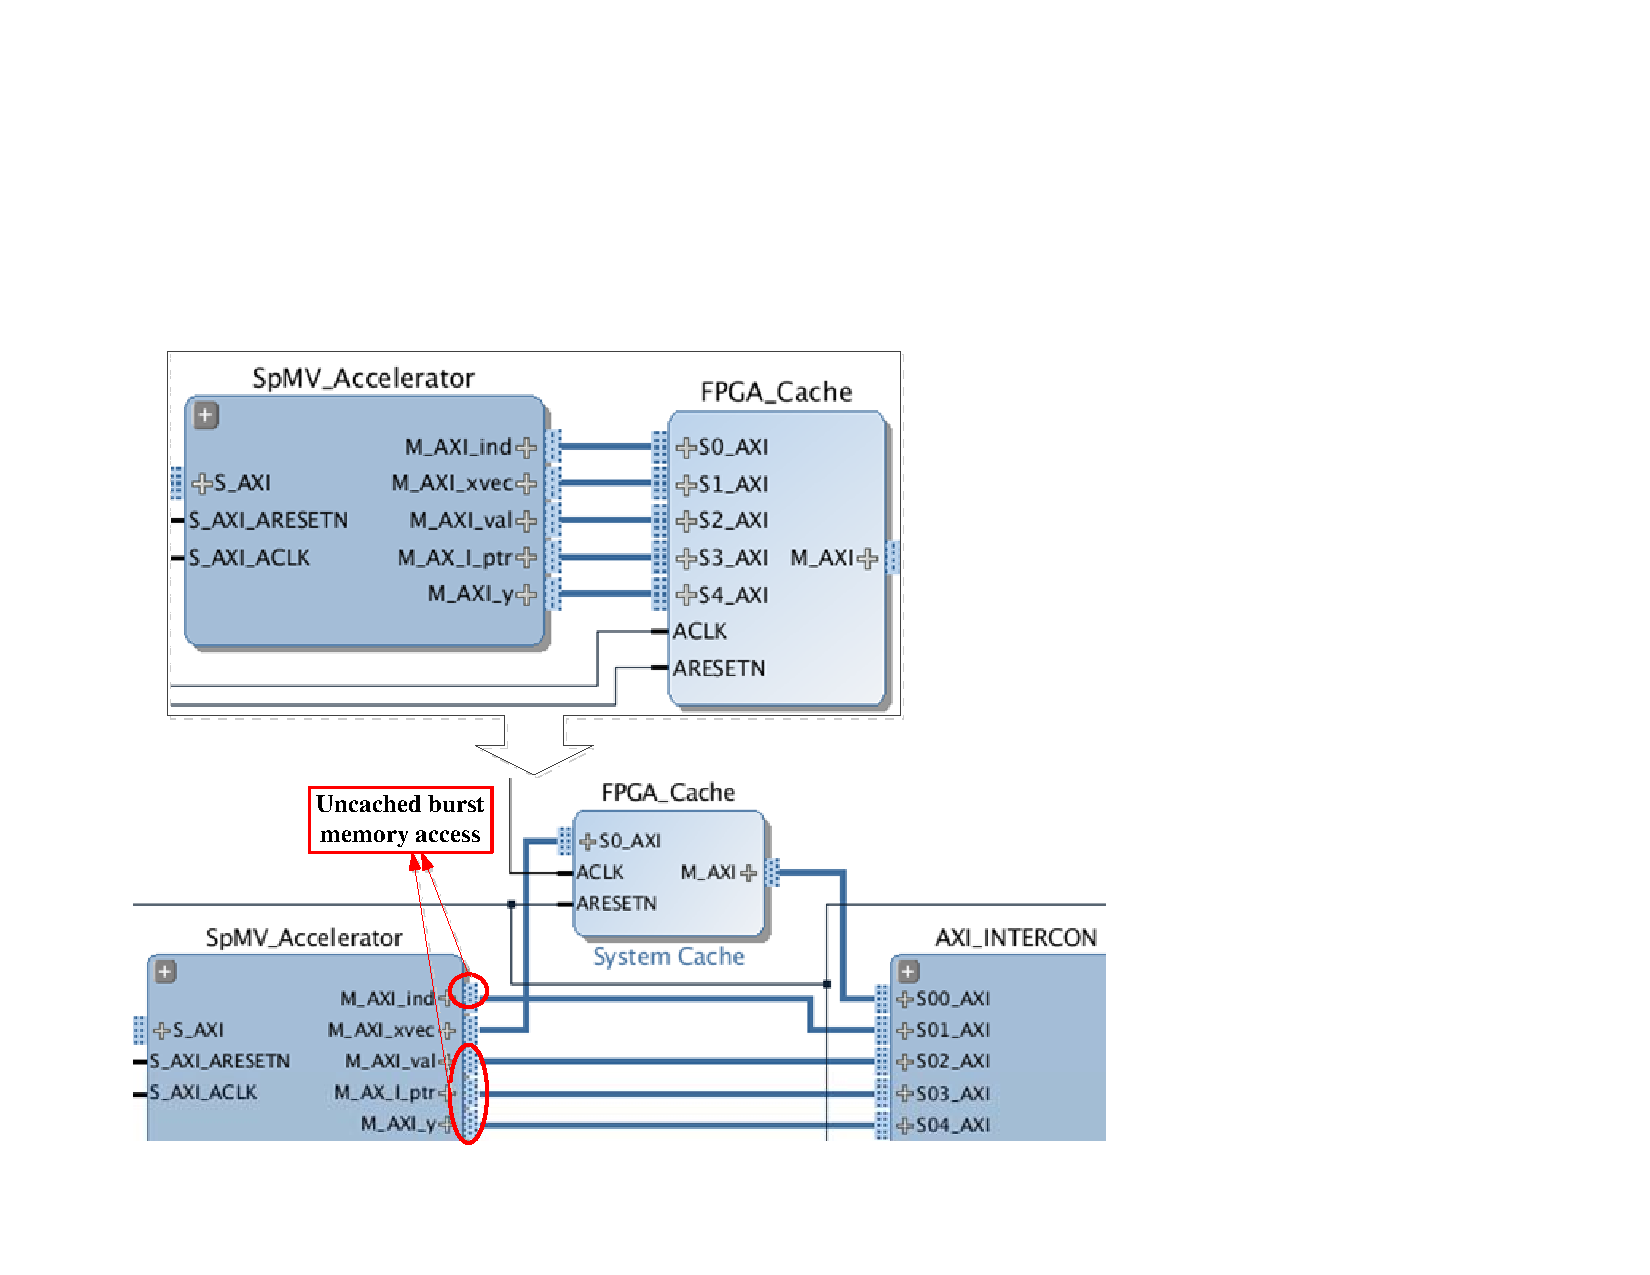
\includegraphics[width=0.65\linewidth]{chap3fig/memOptConv.pdf}
\caption{Optimized Data Access Mechanism
\label{fig:from2}}
\end{center}
\end{figure}
Shown in figure~\ref{fig:from2} is an example where the described techniques are applied to one of our benchmarks.
The cache added between the accelerator and the memory subsystem was originally shared by the five memory
interfaces. However,
as four of those will load/store data in continuous addresses, they can be converted to burst accesses.
The cache is now exclusively used by ``xvec'' which accesses data randomly. The benefits of these transformations
will be quantified in section~\ref{sec:er}.


\section{Hardware Generation}
As mentioned in section~\ref{sec:consp}, LLVM is used for implementing the synthesis flow for the computational pipeline. 
%More specifically, we convert one loop-containing LLVM function into multiple LLVM functions communicating with each other.
To create the final hardware, we translate each of the generated functions back to C syntax and then feed it to an existing HLS tool.

%The original sequential function, which is now a top level wrapper containing invocations of the generated sub
%In essence, we have built a source to source
%transformation flow, 
%taking in one sequential, loop-containing C function and generating multiple C functions, all contained within a .
%To create the RTL implementation from each subgraph,
%we convert these LLVM intermediate representation back to C
%syntax and then feed the obtained function to an existing HLS tool. By building a
%source to source transformation flow, 

%With this functionally equivalent C implementation of the decoupled computational pipeline, We can easily test the result of our
%transformation flow with a software implementation. The portability
%across different back-end HLS tools is also guaranteed.

\subsection{LLVM to C translation}
As the computational pipeline is represented as well formed LLVM IR, it's translation to C is just another LLVM pass we write and apply within the LLVM framework. 


Values in LLVM IR can take on types not recognized by standard C compiler.
For instance, integer types can be of arbitrary width (1-$2^{23}-1$ bits), most of which does not have equivalence in C language. A vast majority of them do not occur
in our flow since the original input is in C. The branch tag tokens and memory
dependency tokens, however, generally have very narrow width. These types
are supported by some HLS tools, but not standard software compilers. Thus we also generate a separate mapping file containing a list of C macros, rounding up the width of the data to one of the standard ones. Consequently, for every synthesized LLVM function, i.e. a stage in the computational pipeline, we can start generating a C implementation which can also be compiled with conventional compilers.

The conversion of functional signature from LLVM to C is rather trivial.
Similarly, at the instruction level, 
%the LLVM to C translation is rather straightforward. 
most of the LLVM IR can be mapped
directly to C statements, as illustrated in figure~\ref{fig:totalFlow}. One
transformation we perform is in dealing with the $\phi$ operations, which generate
 values of variables based on the the incoming control edges.  In the case where the source instruction for an operand is within the same subgraph, instead of
 producing to the operand, this source instruction writes directly to the output
 of the $phi$ operator.
 On the other hand, if the source
is in another subgraph, a load operation is inserted to the basic block
where the data is produced, but again assigning the result directly
to the output variable of $\phi$. The $\phi$
instruction itself can be removed. An example of this conversion is
shown in figure~\ref{fig:phi2c}.
\begin{comment}
To create a well-formed LLVM function, the queue names in the inserted ``push" ``pop" function calls need to be added to the argument list of LLVM functions as pointers. Each of these added pointers is only accessed by a single 

Within each subgraph, the values can take on types not recognized by standard
C compiler. For our flow, this occurs frequently when branch tag tokens or memory
dependency tokens are generated. The 

To create a well-formed LLVM function, the queue names in the inserted ``push" ``pop" function calls need to be added to the argument list of LLVM functions as pointers. Depending on the type of tokens transmitted between functions, data types of non-standard width are sometimes used. This is especially true for some of the integer tokens used (e.g. one bit branch tag token for communicating branch destination). This is supported by LLVM and can be accommodated by some HLS tools, but not the standard C compiler tool chain.
We thus constructed a separate macro mapping file for the software implementation of the generated C, rounding up the with of the data to one of the standard ones. 
\end{comment}




\subsection{Testing with Multithreaded Software Implementation}
We have so far created a C implementation for each
stage in the decoupled computational pipeline. 
%this functionally equivalent C implementation of the decoupled computational pipeline, We can easily test the result of our
%transformation flow with a software implementation. The portability
%across different back-end HLS tools is also guaranteed.
To test the functional equivalence of the synthesized pipeline with the original
function, our flow also creates a multithreaded software implementation using the
$pthread$ library. Each of
the generated stages is assigned to a separate thread, running concurrently with 
all other stages. Channels connecting different stages are implemented as instantiations of a special C++ data structure. An templated array is used to represent a FIFO. A channel can contain multiple arrays when it fans out to
more than one consumer threads. Each array is protected with a mutex and associated
with a conditional variable. Blocking reads and writes are implemented with $pthread\_cond\_wait$ while $pthread\_cond\_signal$ wakes up blocked threads when
token/space becomes available. 

The original sequential function, which has all its computation replaced by
LLVM function invocations, is examined and converted to a top level wrapper. 
It sets up the 


\subsection{Generating System with Xilinx Vivado Tools}
When synthesizing each C functions using Xilinx's Vivado HLS, every pointer argument through which actual memory references occur is converted to a independent memory port. These
are to be connected to the memory subsystem, as will be described later in section~\ref{sec:er}. Other pointer arguments are used for inter-subgraph communication,
they are associated with pragmas directing the creation of FIFO interfaces. In terms of
the scheduling computation in each function, we ensure the inner loops are
all aggressively pipelined, while the barriers are contained in non-inlinable function such that operations are not reordered with respect to them.

\begin{figure}[htp]
\begin{center}
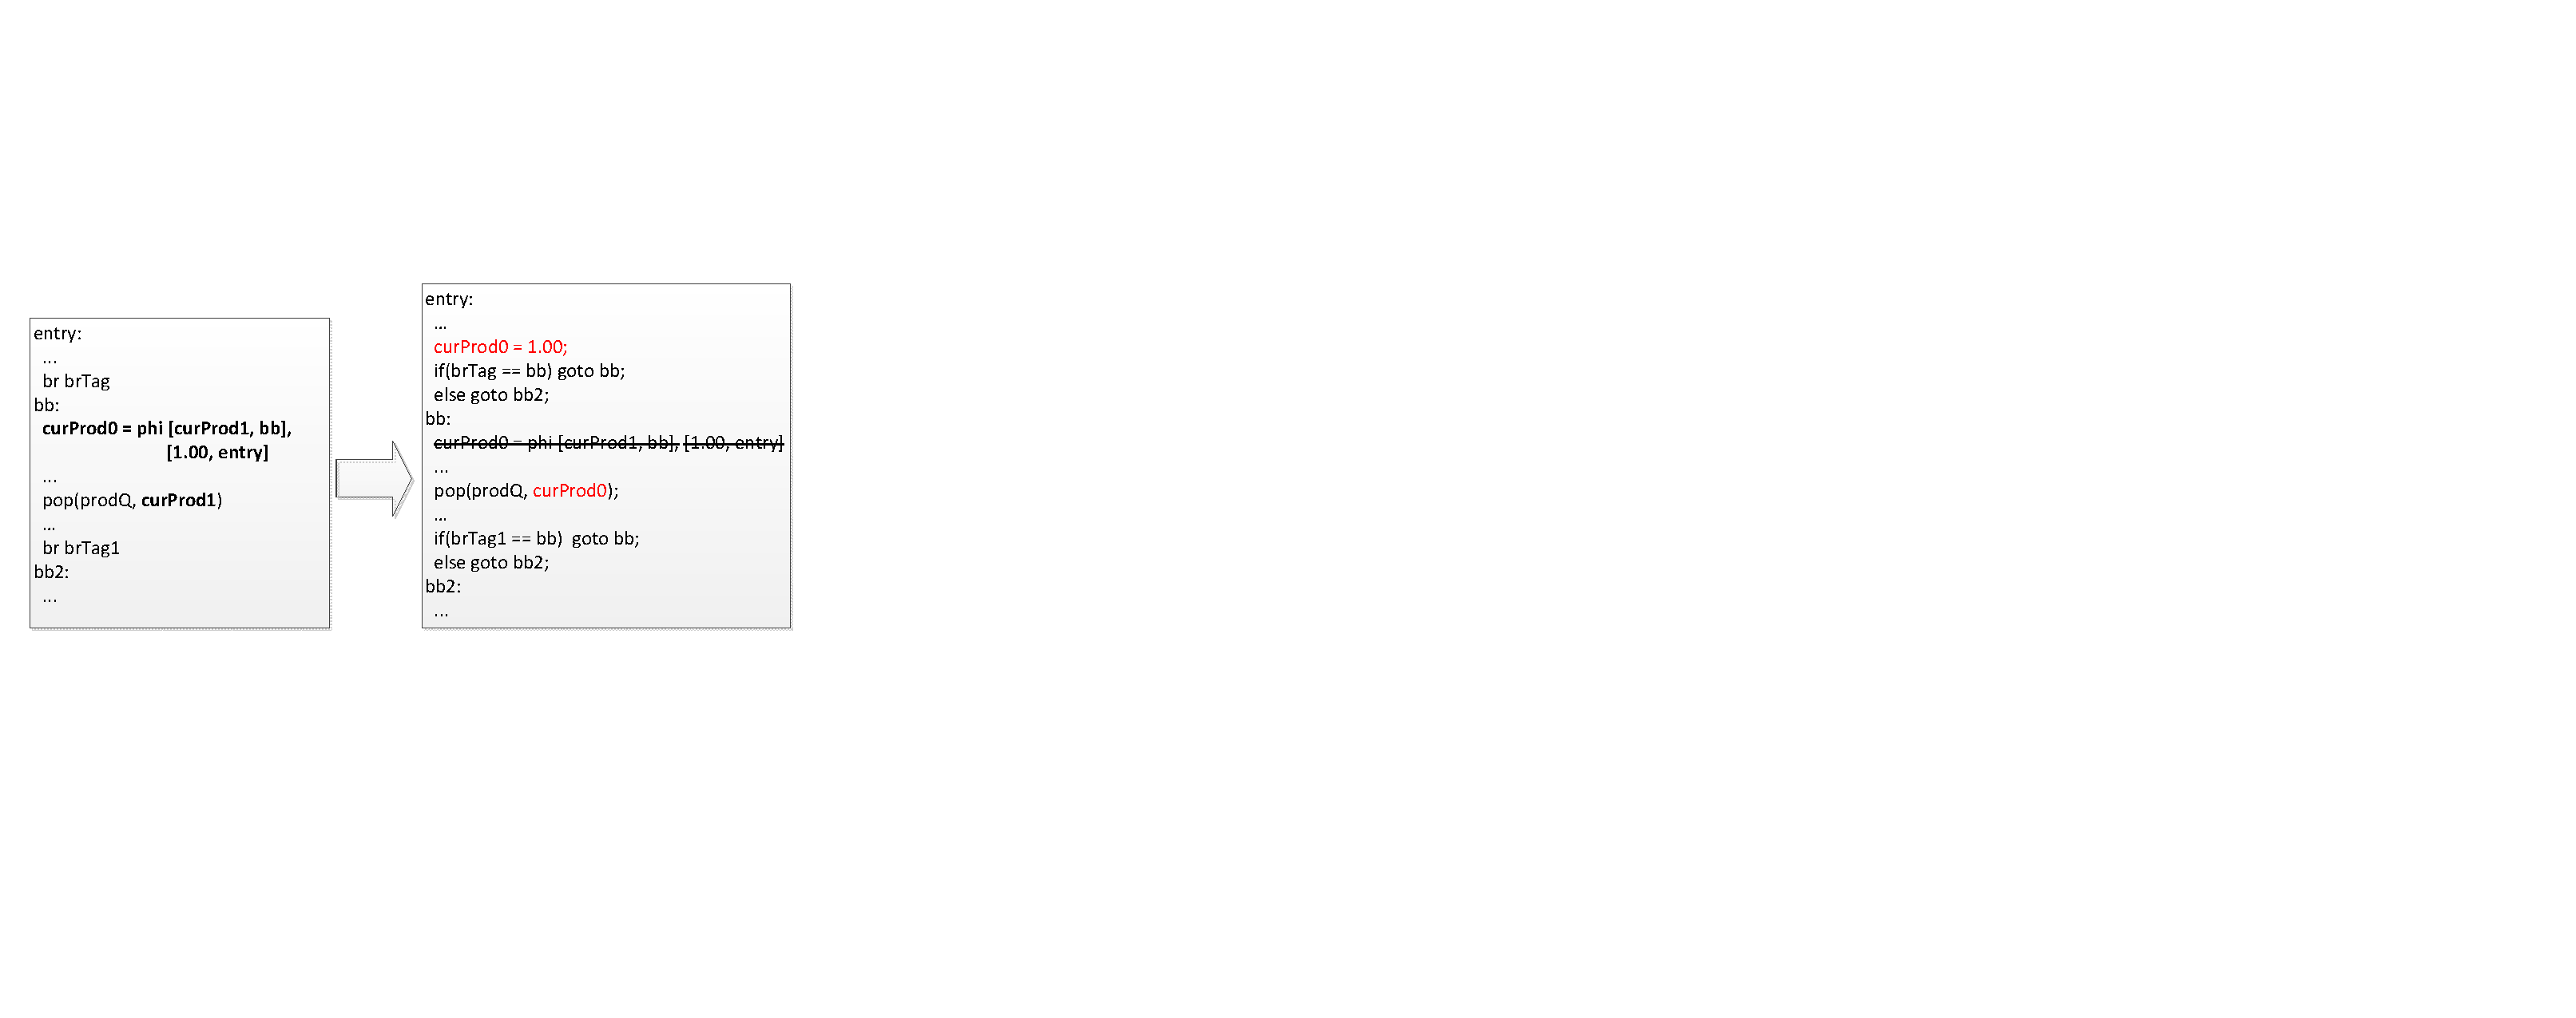
\includegraphics[width=0.7\linewidth]{chap3fig/SSA2C.pdf}
\caption{Converting $\phi$ Operator to C
\label{fig:phi2c}}
\end{center}
\end{figure}


\begin{comment}
As each subgraph contains instructions from only a subset
of the basic blocks in the original program, it does not always
have a complete control flow. To ensure each processing
module generated is self-contained and has well-defined behavior,
extra basic blocks are sometimes added. Our tool finds
the nearest common dominator of all the basic blocks in a
subgraph and add all the control flow statements between this
dominator and the other basic blocks. Consequently, there
is a unique entry block for every subgraph, and different
module will traverse the exact same execution path when the
processing pipeline is active.
\end{comment}

For the next step, where all the components are to be connected
together, we rely on the FIFO generators provided by Xilinx.
Similarly, on-FPGA cache and the
interconnect, which is used to bridge the computational pipeline
and the memory subsystem, are also parametrized Xilinx IPs. 
Within our flow, TCL script is generated according to the communication requirement of the subgraphs. The construction of the whole pipeline
is then performed in Xilinx Vivado IP Integrator by invoking this TCL script.
All the steps involved in our
pipeline generation flow are summarized in figure~\ref{fig:allsteps}.
\begin{figure}[htp]
\begin{center}
\includegraphics[width=0.8\linewidth]{chap3fig/flowSteps.pdf}
\caption{Pipeline Generation Flow
\label{fig:allsteps}}
\end{center}
\end{figure}

%\section{Proof of Liveness}
\section{Experimental Evaluation}
\label{sec:er}
\subsection{Experiment Setup }
To demonstrate the benefits of our approach, processing pipelines
are synthesized and physically implemented on FPGA. The particular device used for the experiments is the Zynq-7000 XC7Z020 FPGA
SoC from Xilinx, installed on the ZedBoard evaluation platform. 
The SoC is divided into two parts: an ARM-processor based processing system (PS), and the programmable logic (PL). 
The baseline 
for our evaluation is the performance of each software kernel running
on the ARM core in the SoC. It is an out of order, dual issue hard
processor running at 667MHz. The Zynq platform also provides two
options for the reconfigurable accelerators to access the main memory subsystem: 
through the accelerator coherence port (ACP), or the high performance (HP) port. 
The former connects to the snoop control unit in the processing system and 
thus uses/modifies the processing system's on chip cache. The HP port connects
directly to the memory controller, which necessitates the flushing of cache lines 
by the processor if a cached data structure is accessed by the accelerator.
In either case, if memory states are also buffered in the reconfigurable array with caches, they 
need to be explicitly pushed to the processing system side after the accelerator finishes running. As both ACP
and HP are slave ports, they provide no mechanisms to extract data from the FPGA
when the ARM processor is running. The interaction between the generated accelerators
and the main pieces of the FPGA SoC is shown in figure~\ref{fig:ippf}.


\begin{figure}[htp]
\begin{center}
\includegraphics[width=0.7\linewidth]{chap3fig/ippf.pdf}
\caption{Implementation of Computational Pipeline in FPGA SoC  
\label{fig:ippf}}
\end{center}
\end{figure} 
In our study, Vivado HLS, a state-of-the-art high level synthesis tool provided by Xilinx,
is used for generating the conventional accelerator (Con.ACC) as well as the individual
modules in our decoupled computational pipeline (DCP). With the target clock period set to 
8ns during HLS, the tightest timing constraints post place \& route implementations managed to meet range from 111 to 150MHz. 
All design points shown in this section 
use the highest achievable frequency as the actual operating clock frequency. 

\subsection{Benchmark Descriptions}
The target application of our flow are algorithms where control flow and
data access patterns depend on run time data or results of computation.
The four irregular kernels listed below are pushed through our flow:
%from several benchmark kernels. These benchmarks
%are non-regular, as their control flow and data access patterns 
%depend on the runtime data. 
\begin{itemize}
    \item \textbf{Sparse matrix vector (SpMV) multiply} is a computation kernel that has been studied, transformed
and benchmarked many different ways in various research projects. Our purpose here is not to produce the best-performing SpMV multiply using special data structure and memory allocation schemes. Rather, we use the most basic and widely used algorithm and storage format to evaluate how much benefit our flow can provide.
The input matrix is stored in
compressed sparse row (CSR) format. 
Loads from
an index array are performed before numbers can be fetched
for the actual floating point multiply. 

\item \textbf{Knapsack } is a problem in combinatorial optimization. Given a collection of
items, each with its own weight and value, knapsack tries to select a subset of them such that the total profit is maximized while the weight limit is not violated.
It is a classic problem which is often solved using dynamic programming, where the memory addresses accessed come from computation.
It is therefore hard to prefetch the needed data unless the entire dataset fits
in on chip buffer.
%only available during run time, and therefore the exact locations where the variable opt_without is loaded from are not known a priori. 

\item \textbf{Floyd-Warshall} takes a graph as input and computes the shortest distances between any pairs of vertices. Similar to knapsack, it is solved by
dynamic programming. Even though all memory references are regular, i.e. simple functions of the loop indices, the control flow depends on the results of computation.

\item \textbf{Iterative depth first search} is again a widely used graph algorithm. The version used for our experiment makes use of a stack and operates on pointer based data structures. 
 
\end{itemize}

The irregularity in
memory accesses and execution paths in these benchmarks makes it hard for existing
HLS tools to directly generate efficient hardware. The conventional accelerators, when
implemented on the FPGA, are also very sensitive to the latency
of data accesses, due to the high ratio of memory operations to computation.

\begin{table}[htbp]
\caption{Input Data Set for the Benchmarks}
\centering
\begin{tabular}{| c | c | c | }
  \hline            
  
 \multirow{2}{*}{Benchmark}   &   \multirow{2}{*}{Description of Input Data} & \multirow{2}{*}{Total Size of Input Data}\\
 &       &   \\
  \hline            
  \hline            
\multirow{2}{*}{}SpMV&  Matrix dimension = 4096 & \multirow{2}{*}{ $\approx$ 16 MB}  \\
%\cline{2-3}                                                                                                                                                    
 Multiply &Density of Matrix = 0.25       &  \\
%\cline{2-3}                                                                                                             
   \hline                                                                                                           
\multirow{2}{*}{Knapsack}&  Weight Limit = 3200 &\multirow{2}{*}{$\approx$ 5 MB}  \\
%\cline{2-3}                                                                                                                                                    
  &Number of Items = 200       &   \\
%\cline{2-3}                                                                                                             
\hline
\multirow{2}{*}{}Floyd-& \multirow{2}{*}{Number of Nodes = 1024}  & \multirow{2}{*}{$\approx$ 8 MB}  \\
%\cline{2-3}                                                                                                                                                    
 Warshall &       &   \\
%\cline{2-3}                                                                                                             
\hline
\multirow{2}{*}{}Depth-First&  Number of Nodes = 4000 & \multirow{2}{*}{$\approx$ 3 MB}  \\
%\cline{2-3}                                                                                                                                                    
 Search & Number of Neighbors per Node = 200       &   \\
%\cline{2-3}                                                                                                       
  \hline                                                                                                           
\end{tabular}
\label{tab:datasize}
\end{table}


Table~\ref{tab:datasize} describes the characteristics of the input data set for each
benchmark. 
As our approach is primarily used for cases where off-chip communication plays a
significant role in determining the final performance, the input data size are chosen
to be much larger than typical on-FPGA cache. For smaller problems where the
entire input data set can be buffered on chip, the conventional DMA+accelerator approach,
as described in~\cite{vivado_hls:appnoteMMult}, would not suffer from variable data access
latency and our decoupled computational pipelines would offer little advantage.




\begin{figure}[htp]
\begin{center}
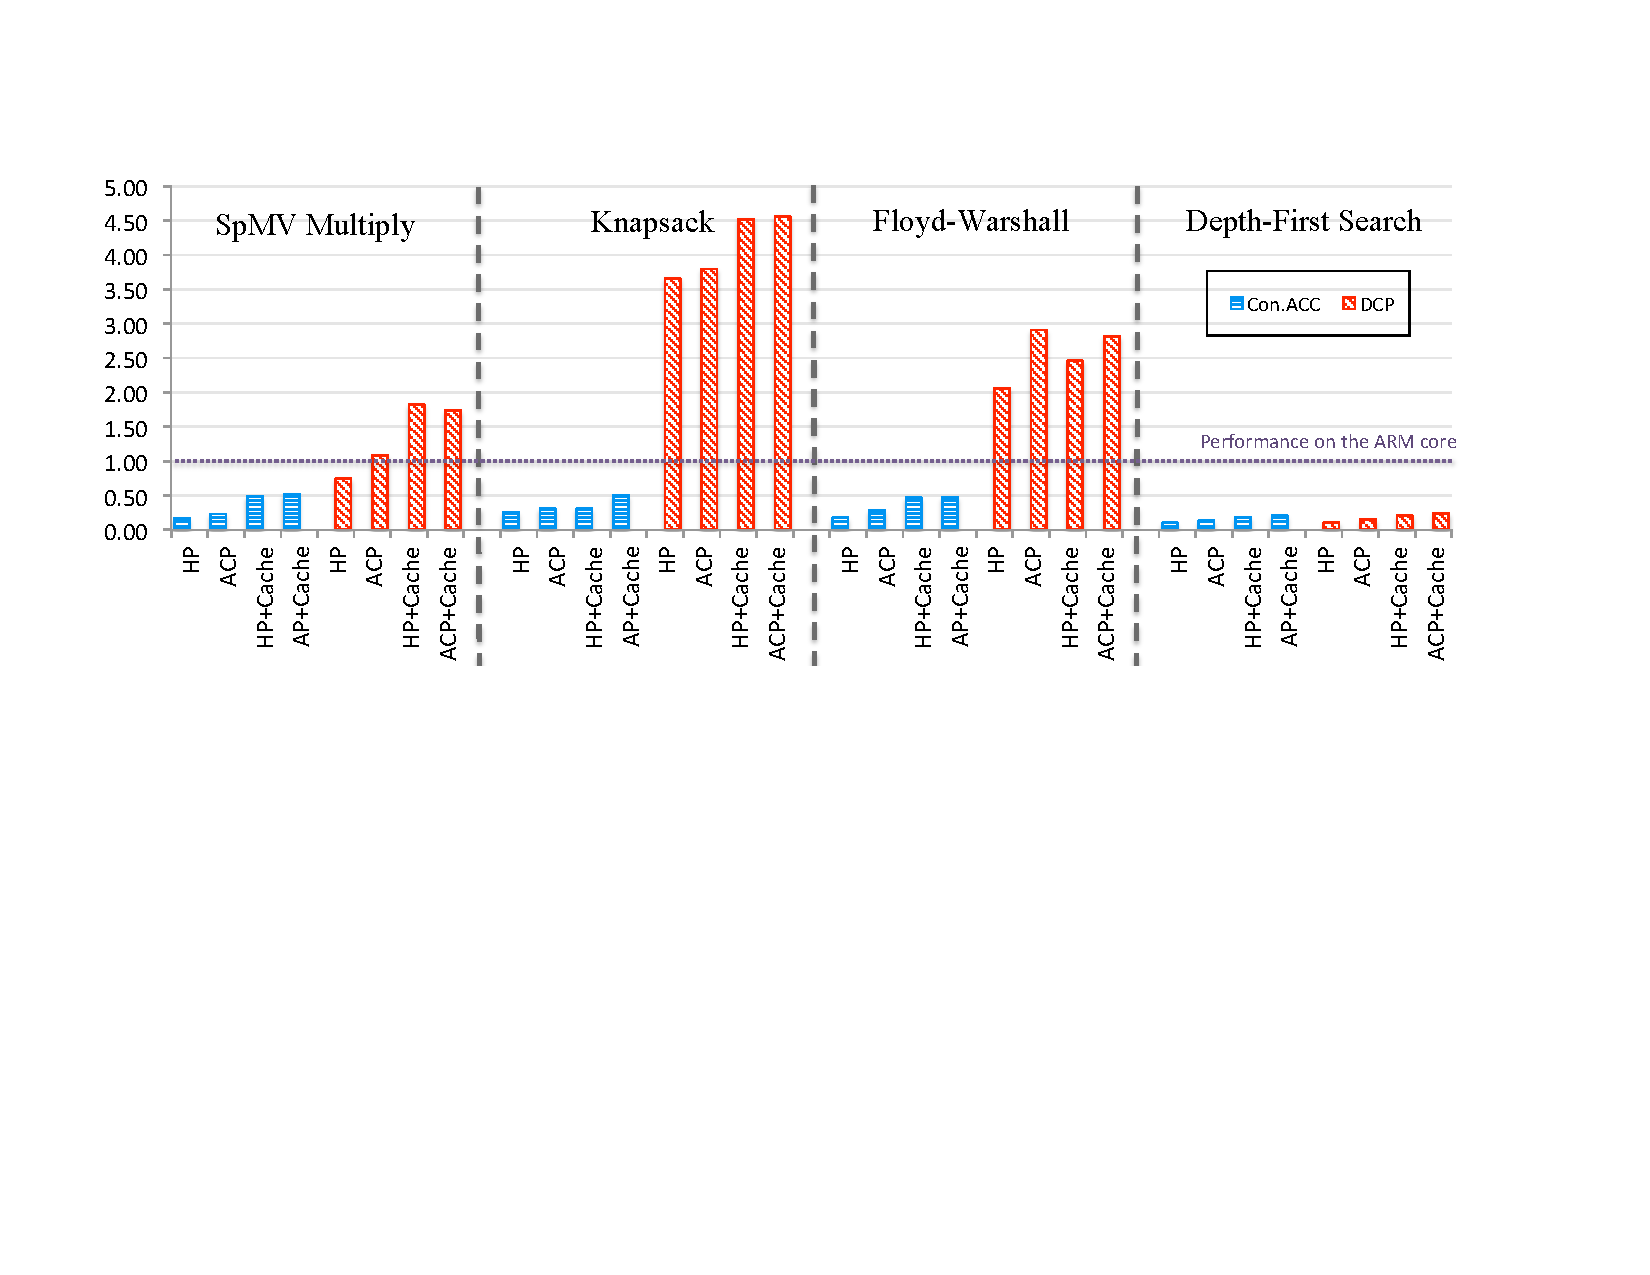
\includegraphics[width=1.0\linewidth]{chap3fig/thesis_perf.pdf}
\caption{Performance of Conventional Accelerators and Decoupled Computational Pipelines
\label{fig:acpraw}}
\end{center}
\end{figure}



\subsection{Performance Comparisons}
\begin{comment}
To provide context for our comparison and highlight the weakness of accelerators generated directly using HLS, we show the performance of a set of conventional accelerators in figure~\ref{}. All the numbers in the figure are normalized to the baseline (software running
on hard ARM core).

These conventional accelerators are supported with different configurations of the memory subsystem. Direct connection to HP port generally incurs the highest memory access latency as
the data are not cached in the PS or the PL. The latency is reduced when ACP is used. To
bring the data even closer to the accelerator, caches can be instantiated on PL. Our implementations use Xilinx system cache IP, configured to be 64KB and 2 way associative.

From this figure, there is a very clear trend that the overall performance increases significantly as the data get cached closer to the accelerators. Across the four benchmarks, the ratio of the fastest to the slowest design points is, on average, 2.4x. The throughput is apparently rather sensitive to the memory access latency. Meanwhile, even the fastest configurations here are slower compared to the baseline. With caches on PL, the conventional accelerators, on average, only achieves throughput about 40\% that of the baseline.
The superscalar, out-of-order ARM core is capable of exploiting instruction level parallelism to a good extent and also has a high performance on-chip cache.
The additional parallelism extracted by the HLS tool is evidently not enough
to compensate for the clock frequency advantage the hard processor core has over the programmable logic and the longer data access latency from the reconfigurable array. 


Now we look at the performance of the decoupled computational pipelines (figure~\ref{}).
Similar to the conventional accelerators, these pipeline's throughput also increase
as the data latency reduces. However, the differences between the different memory subsystem
configurations are significantly smaller. The fastest configuration is only 1.7x better than 
the slowest, which demonstrate how the effect of data access latency is reduced in our
generated pipelines. Also, compared to the baseline, the DCPs provide much better performance.
On average, the 

To highlight the difference in raw performance, the fastest conventional accelerators and the decoupled computational pipelines are compared side by side in figure~\ref{}. There is a very
clear performance advantage



To understand the pros and cons of different optimization options and support infrastructure configurations, we have generated an array of different design points for each benchmark.
Every design point represents a different trade off between performance and area cost. 

\subsubsection{Sparse Matrix Vector Multiply}
Sparse matrix vector (SpMV) multiply is a computation kernel that has been studied, transformed
and benchmarked many different ways in various research projects. Our purpose here is not to produce the best-performing SpMV multiply using special data structure and memory allocation schemes. Rather, we want to see, given the most basic and widely used algorithm description, how
much benefit our flow can provide.

To provide 

We want to examine how the partitioning of operations and the subsequent optimization affect the performance and area. Here we connect a few different instances of the DCPs generated to the HP port of the processing system, and compare them against the directly generated Con.ACCs.


Figure~\ref{}, shows the performance and area of a few design points
\end{comment}

In figure~\ref{fig:acpraw}, performance of the conventional accelerators and decoupled computational pipelines are compared, all the numbers are normalized to the baseline.
Both Con.ACC and DCPs are supported with different memory subsystem configurations.
%Conventional accelerators and decoupled computational pipelines with different memory subsystem
%configurations are compared.  
Direct connections to the HP port generally incur the highest memory access latency as
the data are not cached in the PS or the PL. This latency is reduced when ACP is used. To
bring the data even closer to the accelerator, cache IPs can be instantiated on the PL. Our implementations use Xilinx's system cache IP, configured to be 64KB and 2 way associative.


In all four benchmarks, accelerators generated directly from software kernels using conventional HLS flow
actually result in a performance degradation compare to running the kernels on the hard processor. The fastest Con.ACC implementations with
on-PL caches, only manage to achieve throughput less than 50\% that of the baseline. 
The superscalar, 
out-of-order ARM core is capable of exploiting instruction level parallelism to a good extent 
and also has a high performance on-chip cache.
The additional parallelism extracted by the HLS tool is evidently not enough
to compensate for the clock frequency advantage the hard processor core has over the programmable logic and the longer data access
latency from the reconfigurable array. 

With our methodology, the computational pipelines generated 
are rather competitive against the hard processor, even
without a reconfigurable cache. For SpMV multiply, knapsack and Floyd-Warshall, when DCPs are directly connected to the PS through the ACP, 
the average performance is 2.3 x that of the baseline---representing
an 8.4 x gain over the conventional accelerators.
Upon the addition of on-PL caches,  
the average runtime of DCPs was further reduced by 18.7\%, making the DCPs about 2.9x faster than the baseline.

It is also apparent that our approach has its limitations, as demonstrated by its ineffectiveness in the benchmark depth first search.
The kernel performs very little computing but lots of memory accesses.
The use of a stack in DFS also creates a dependence cycle through the memory
and consequently, the performance is fundamentally limited by the latency of memory access.
Thus there were only small differences between the performance of the conventional accelerator and the decoupled computational pipeline. Besides, the memory access pattern
does not provide many opportunities for optimizations. As a result, DCP and Con.ACC achieves performance far below that of the baseline, 
which has a much higher clock frequency and a faster cache.     


The figure also allows us to examine the effect of different memory configurations on the overall performance of the design. There is a general trend that the performance improves as the 
data get cached closer to the computation engine. For conventional accelerators, the ratio of the fastest to the slowest design points is, on average, 2.4x. For decoupled computational pipeline,
this ratio is reduced to 1.7x. The relative insensitivity of the DCPs towards data access latency
is rather evident from this difference.
\begin{comment}
The throughput is apparently rather sensitive to the memory access latency.

while that of the conventional
accelerators was cut by 45.4\%. The gap between their performance is thereby reduced from 8.4 to 5.6 times. 
%This difference is due to conventional accelerators' sensitivity to the latency of data accesses, which
%is also manifested by its performance degradation of 40\% when the uncached HP port is used instead of ACP. 
\end{comment}

Overall, for kernels suitable for FPGA acceleration, there is a significant performance advantage in using
decoupled computational pipelines. If we compare the best results using DCP to conventional accelerators, we see improvement
of 3.3 to 9.1 times, with an average of 5.6. 

\begin{table}[htbp]
\caption{Resource Usage of Accelerators.}
\centering
\begin{tabular}{| c | c | c | c | c | c | c | c| }
  \hline            
  \multirow{2}{*}{} &  &   \multicolumn{3}{c|}{ACP  } & \multicolumn{3}{c|}{ ACP + 64KB Cache }   \\
 \cline{3-8} 
 {Benchmark}   &    & LUT& FFs& BRAM & LUT &	 FFs    	& BRAM    \\
  %
  %                 & LUT &FFs&  BRAM &  LUT &	 FFs    	& BRAM   \\
  \hline            
  \hline            
\multirow{3}{*}{}&Con.ACC  & 9873 &9116 &10 & 7918 & 6792 & 21  \\
\cline{2-8}                                                                                                                                                    
SpMV &DCP       & 8577 & 8837& 10 & 6718  &6788 & 21\\
\cline{2-8}                                                                                                             
    Multiply   &\% change & -13.1 &-3.1 & 0 & -15.2  & -0.1 & 0  \\
  \hline                                                                                                           
\multirow{3}{*}{}&Con.ACC  & 7672 &7490 &8 & 6573 & 5885 & 21  \\
\cline{2-8}                                                                                                                                                    
Knapsack &DCP       & 8089 & 8787& 8 & 6970  &7256 & 21\\
\cline{2-8}                                                                                                             
       &\% change & +5.4 &+17.3 & 0 & +6.0  & +23.3 & 0  \\
  \hline                                                                                                           
\multirow{3}{*}{}&Con.ACC  & 2491 &3528 &0 &3806  &4629  &19   \\
\cline{2-8}                                                                                                                                                    
Floyd- &DCP       & 7659 &7210 &0  &8995  &8309 &19 \\
\cline{2-8}                                                                                                             
 Warshall      &\% change &+207.5  &+104.3 & 0 & +104.4  & +79.5  & 0  \\
  \hline                                                                                                           
\multirow{3}{*}{}&Con.ACC  & 4810 &4929 &4 & 4931 & 4594 & 21  \\
\cline{2-8}                                                                                                                                                    
DFS &DCP       & 8509 & 7813& 4 & 7436  &6298 & 21\\
\cline{2-8}                                                                                                             
       &\% change & +76.9 &+58.5 & 0 & +50.8  & +37.1 & 0  \\
  \hline                                                                                                           

\end{tabular}
\label{tab:areacom}
\end{table}







\subsection{Area comparison}
To quantify the impact of our proposed methodology on area, 
we have compared the FPGA resouce usage of conventional accelerators and
the decoupled computational pipelines.
Table~\ref{tab:areacom} shows the results, 
where each acclerator is complemented with two different memory subsystem configurations.

The difference in area between DCPs and Con.ACCs is effected by
two factors.  There are additional costs associated with the communication primitives 
and FIFOs for the DCP implementations. 
On the other hand,   
the original programs are partitioned into subgraphs and separately turned into hardware
in DCPs, which sometimes can reduce the depth of the internal 
pipeline in the processing modules, resulting in area savings. 
%as compared to the instantiation
%of the same set of operators in conventional accelerators. 
%For instance,
%in our motivating example, the initiation interval of the inner loop is 
%determined by the floating point multiply. The loop counter, which is
%another SCC in our dataflow, will also need
%to be synchronized to the same schedule, which necessitate insertion of
%additional pipeline stages. 
The overall change therefore depends on which factor plays a larger role, and is 
ultimately application specific. 


\section{Discussion and Future Work}
The experimental results have validated the general approach we have proposed and implemented. 
Decoupling of execution between different part of the control dataflow graph can yield
significant benefits. With different parts of the graph each having their own controller, non-statically schedulable stalls get isolated and more opportunities for
optimization can be exploited. Unfortunately, these benefits do not come for free. We observed significant area increase when generating our decoupled computational pipeline.
How to strike the right balance between performance gain and the area cost by devising different ways to partition the CDFG is an interesting dimension for future exploration.

The algorithm we have implemented in this chapter is rather simplistic. 
It is also very aggressive in that all separable memory accesses are assigned to a new partition.
Furthermore, as we perform topological sort on the nodes before partitioning them, many
edges might be cut when a new subgraph is created, especially when the dependencies between instructions are relatively denser.
Therefore, as the input kernels increase in size, our algorithm may result in pipelines with prohibitively high number of communication channels. The optimization we described in section~\ref{dupvscomm}
partially addresses this issue, but it does not reduce the total number of subgraphs.

A more general framework, the application of which is left for future work, involves the


\begin{comment}
To alleviate this particular issue, we can make the whole pipeline generation process more
flexible. While the instruction partitioning step can be changed and various techniques can be
experimented with, the construction of executable subgraphs and the synthesis of hardware
are invariant across different partitioning schemes. Optimizations like pipelining of memory
requests can still be applied if it can be accommodated by the structure of the reconstructed
subgraphs. Within this context, several possible partitioning heuristics may be worth trying out
in the future.

The algorithm we have implemented ensures the data tokens always flow forward, as the
partitioning is performed on a directed acyclic graph. The benefit si
\end{comment}

\chapter{Decoupled Computational Pipeline as a Process Network}
\label{liveprof}
To facilitate the analysis of the pipeline of subgraphs generated from the original sequential program,
we relate it to a different model of computation, Kahn process network(KPN). which
provides the theoretical context for looking at issues such as deadlock and FIFO sizing in our pipeline. 


The KPN is an inherently
parallel model of computation where processes communicate with
each other through unbounded FIFO channels. 
The processes cannot test for availability of data tokens in 
the channels without consuming them. If a channel is empty
the process blocks as it reads from the channel.
Writing to the FIFOs, however, is non-blocking.
In addition, each FIFO can only be consumed by a single process, and be written to by a single process. The KPN model is deterministic in the sense that the scheduling of
the process execution does not alter the final results. This gives great flexibility
in implementing/controlling each individual processes. 
By relating our pipeline to KPN, or more precisely, observing its deviation from a pure
KPN, we can understand the freedom we have and the constraints we are subjected
to in our synthesis flow, where the correctness and liveness of the final implementation is required. Note the required absence of deadlock does not
apply to the eventual state of our pipeline, when the execution finishes.
As mentioned in section~\ref{sec:consp}, the execution of the pipeline completes when all subgraphs are either done running or waiting for inputs, which is a form of deadlock. This is expected and not the subject of our discussion in this
chapter.


%The generation of decoupled subgraphs from the original CDFG can actually be seen as a procedure which generates a more restricted version of KPN from sequential programs.
%As the shared global memory accesses do not fit into the KPN model naturally,
%we will have to first bridge this gap in their semantics(section~\ref{mp}). In implementing the network, we inevitably have to confront the boundedness of the
%FIFO channels, which may create deadlock situation depending on how each process
%are executed locally. We provide an analysis of the issue in  


\section{Memory and Fanout Process}
\label{mp}
A characteristic
of KPN is that all data exchange are performed over the FIFOs and the notion of
a shared global memory does not exist in the model. Previous works
converting sequential programs to process networks~\cite{mat2pn}\cite{c2stream}
were able to transform the original memory operations to explicit data IOs
at the boundary of the generated hardware as the targeted kernels are highly 
regular. In our case however, the synthesized pipelines may have irregular memory access patterns and are often used as accelerators along side a general purpose processor, the memory model needs to be preserved. It is therefore necessary to conceptually
translate the behavior of processes accessing memory to that of inter-process
communication.
%This is
%especially important as the generated accelerator is used in 
%conjunction with a general purpose processor which also shares
%the same memory subsystem. In another word, we need to 
%preserve the memory model in implementation but conceptualize
%the accesses in terms of distributed processes to allow for analysis.
%This is one area which was not addressed in previous works which 
%attempted to convert sequential programs to  process networks~\cite{mat2pn}\cite{c2stream}. They were targeting highly regular kernels where it is possible to
%have the original memory operations transformed to explicit data
%IOs at the boundary of the accelerator. In our case, however, the individual processes still access the shared memory directly, and we need to translate this behavior
%into that of communicating processes. 


In our system, the memory subsystem, including the associated interconnects, exposes multiple
input and output ports to the other hardware modules. 
Just like other processes in the network, through these ports, it consumes and produces tokens. In the case of load operations, addresses generated by the other processes
are read by the memory, and the corresponding data are returned. For store operations, on the other hand, the memory
consumes an extra data token while returning an acknowledge token.
This is certainly not sufficient to allow us to model it as
a conventional process in the network.
In particular, while a normal process blocks when reading from an empty
channel, the absence of requests at one input port never prevents the memory from serving requests from other ports. In another word, it can choose
which port to read depending on the availability of input tokens.
In YAPI~\cite{}, a ``select" function is added as an extension to the Kahn process network to support non-deterministic events. The behavior of
the shared memory subsystem can be accommodated with this primitive as well. 

With the introduction of ``select", the semantics of the original KPN is violated.
The memory subsystem can produce different output sequence depending on
the relative timing of appearance of token at its different input ports. 
This implies the scheduling of other processes would have an effect on the final
result of the execution, the system is no longer deterministic. 
However, as described in section~\ref{sec:partins}, we partitioned the memory
address space and added special memory-dependency edges between instructions. Consequently, the timing of memory requests coming from the normal processes are coordinated by the sending and receiving of special tokens among themselves.  This added constraint effectively eliminated any input token
sequences inconsistent with the behavior of the original sequential program,
while presenting the deviant memory ``process" a strict subset of the possible inputs. 
With the input streams across
different ports adhere to the read-after-write, write-after-read and write-after-write requirements encoded in the memory access instructions of the original program, the system becomes deterministic again. 

\begin{comment}
Thus we need 
to devise a mechanism such that only a certain subset of all possible input sequences
can ever be observed by the memory subsystem, and this subset would always result
in sequences of output tokens consistent with the behavior of the original sequential program.
%and this subset would always result
%in the same sequence of output tokens which is also consistent with the behavior of the %original sequential program. 
This is achieved by putting constraints on
the address/data streams generated by each process, which is in turn realized
by partitioning the address space and adding special memory-dependency edges between instructions, as mentioned in
chapter~\ref{sec:partins}. 
\end{comment}

\begin{figure}[htp]
\begin{center}

\includegraphics[width=0.85\linewidth]{chap4fig/memProcess.pdf}
\caption{Modeling Memory Access as Inter-process Communication
\label{fig:memproc}}
\end{center}
\end{figure}

In denotational semantics of KPN, each process is defined as a function mapping potentially infinite input streams to output streams, independent of the relative timing
of tokens in the streams.
After eliminating the possibility of the conventional
processes generating request sequences which violates memory dependency constraints, for all practical purposes, the memory subsystem can be seen as exactly that. 
%With 
%multiple input ports and multiple output ports however, 
%it cannot be described
%as a simple sequential process with blocking read, since the absence of requests at one port never prevents the memory from serving request from other ports. 
We can 
model it as a deviant process with no blocking read who, when scheduled, always takes a new request token and produces response/acknowledge token. This concept is visualized in figure~\ref{fig:memproc}. In particular, there is no sequential
ordering between the two response block $R1$ and $R2$, though within each block,
the operations are strictly ordered.






%we can see the memory subsystem as a process in the network whose
%output sequences do not depend on the scheduling of the network.  
%In denotational semantics of KPN, each process is defined as a function mapping %potentially infinite input streams to output streams. We can see the memory
%exactly as this mapping function when all the possible input streams across
%different ports adhere to the read-after-write, write-after-read and write-after-write requirements encoded in the memory access instructions of the original program. FIXME:adding picture for memory process 

%
%In the most trivial case, where each memory access operation in the original
%program is targeting a different part of the address space, the memory can
%be modeled as many little processes, each of which communicates with one memory %access
%operation in the process network, as shown in figure~\ref{}. This is however, an %unrealistic
%scenario, the memory is used for compute operations to communicate with each other
%temporally, therefore the accessed regions, more often than not, overlap with
%each other. 
%At the other end of the spectrum, we assume all the memory accesses
%are targeting the same memory location and all read-after-write, write-after-read
%and write-after-write ordering must be preserved, i.e. with a lot of memory-dependency-edges added in our CDFG. In this scenario, the memory
%can be modeled as one single process, who is only going to see
%the input sequences consistent with the order
%of memory accesses in the original program, and the sequences of tokens at each
%output port will be such that the actual 

%As mentioned in chapter~\ref{decoupleChap},  

%To model
%Given a specific input (token) history for a process, the process must be deterministic so that it always produces the same outputs (tokens)

%Given the partition of the memory address space, we can model each
%partition as 
%



Another requirement for KPN is the singularity of producers and consumers
for each channel. However, in a typical program represented in single static assignment form, value defined by an instruction can be used by multiple consumer instructions. 
To make it compatible with the KPN model, explicit fanout processes are added.
For every $1-to-n$ def-use relationship in the SSA, a fanout process with one
input and $n$ outputs is added. The process duplicates every input token $n$ times and sends one to each of the consumer processes. 
As shown in figure~\ref{fig:fanout}, a
fanout process, just like other processes created from partitioning CDFGs, consists
of a sequence of instructions, some of which consume tokens while others produce and transmit tokens. 
With the addition of these processes all the channels in the network are one to one and we have a conceptualization of the entire computation described by the original program
in terms of a KPN, with the addition of a more flexible memory ``process''.

\begin{figure}[htp]
\begin{center}
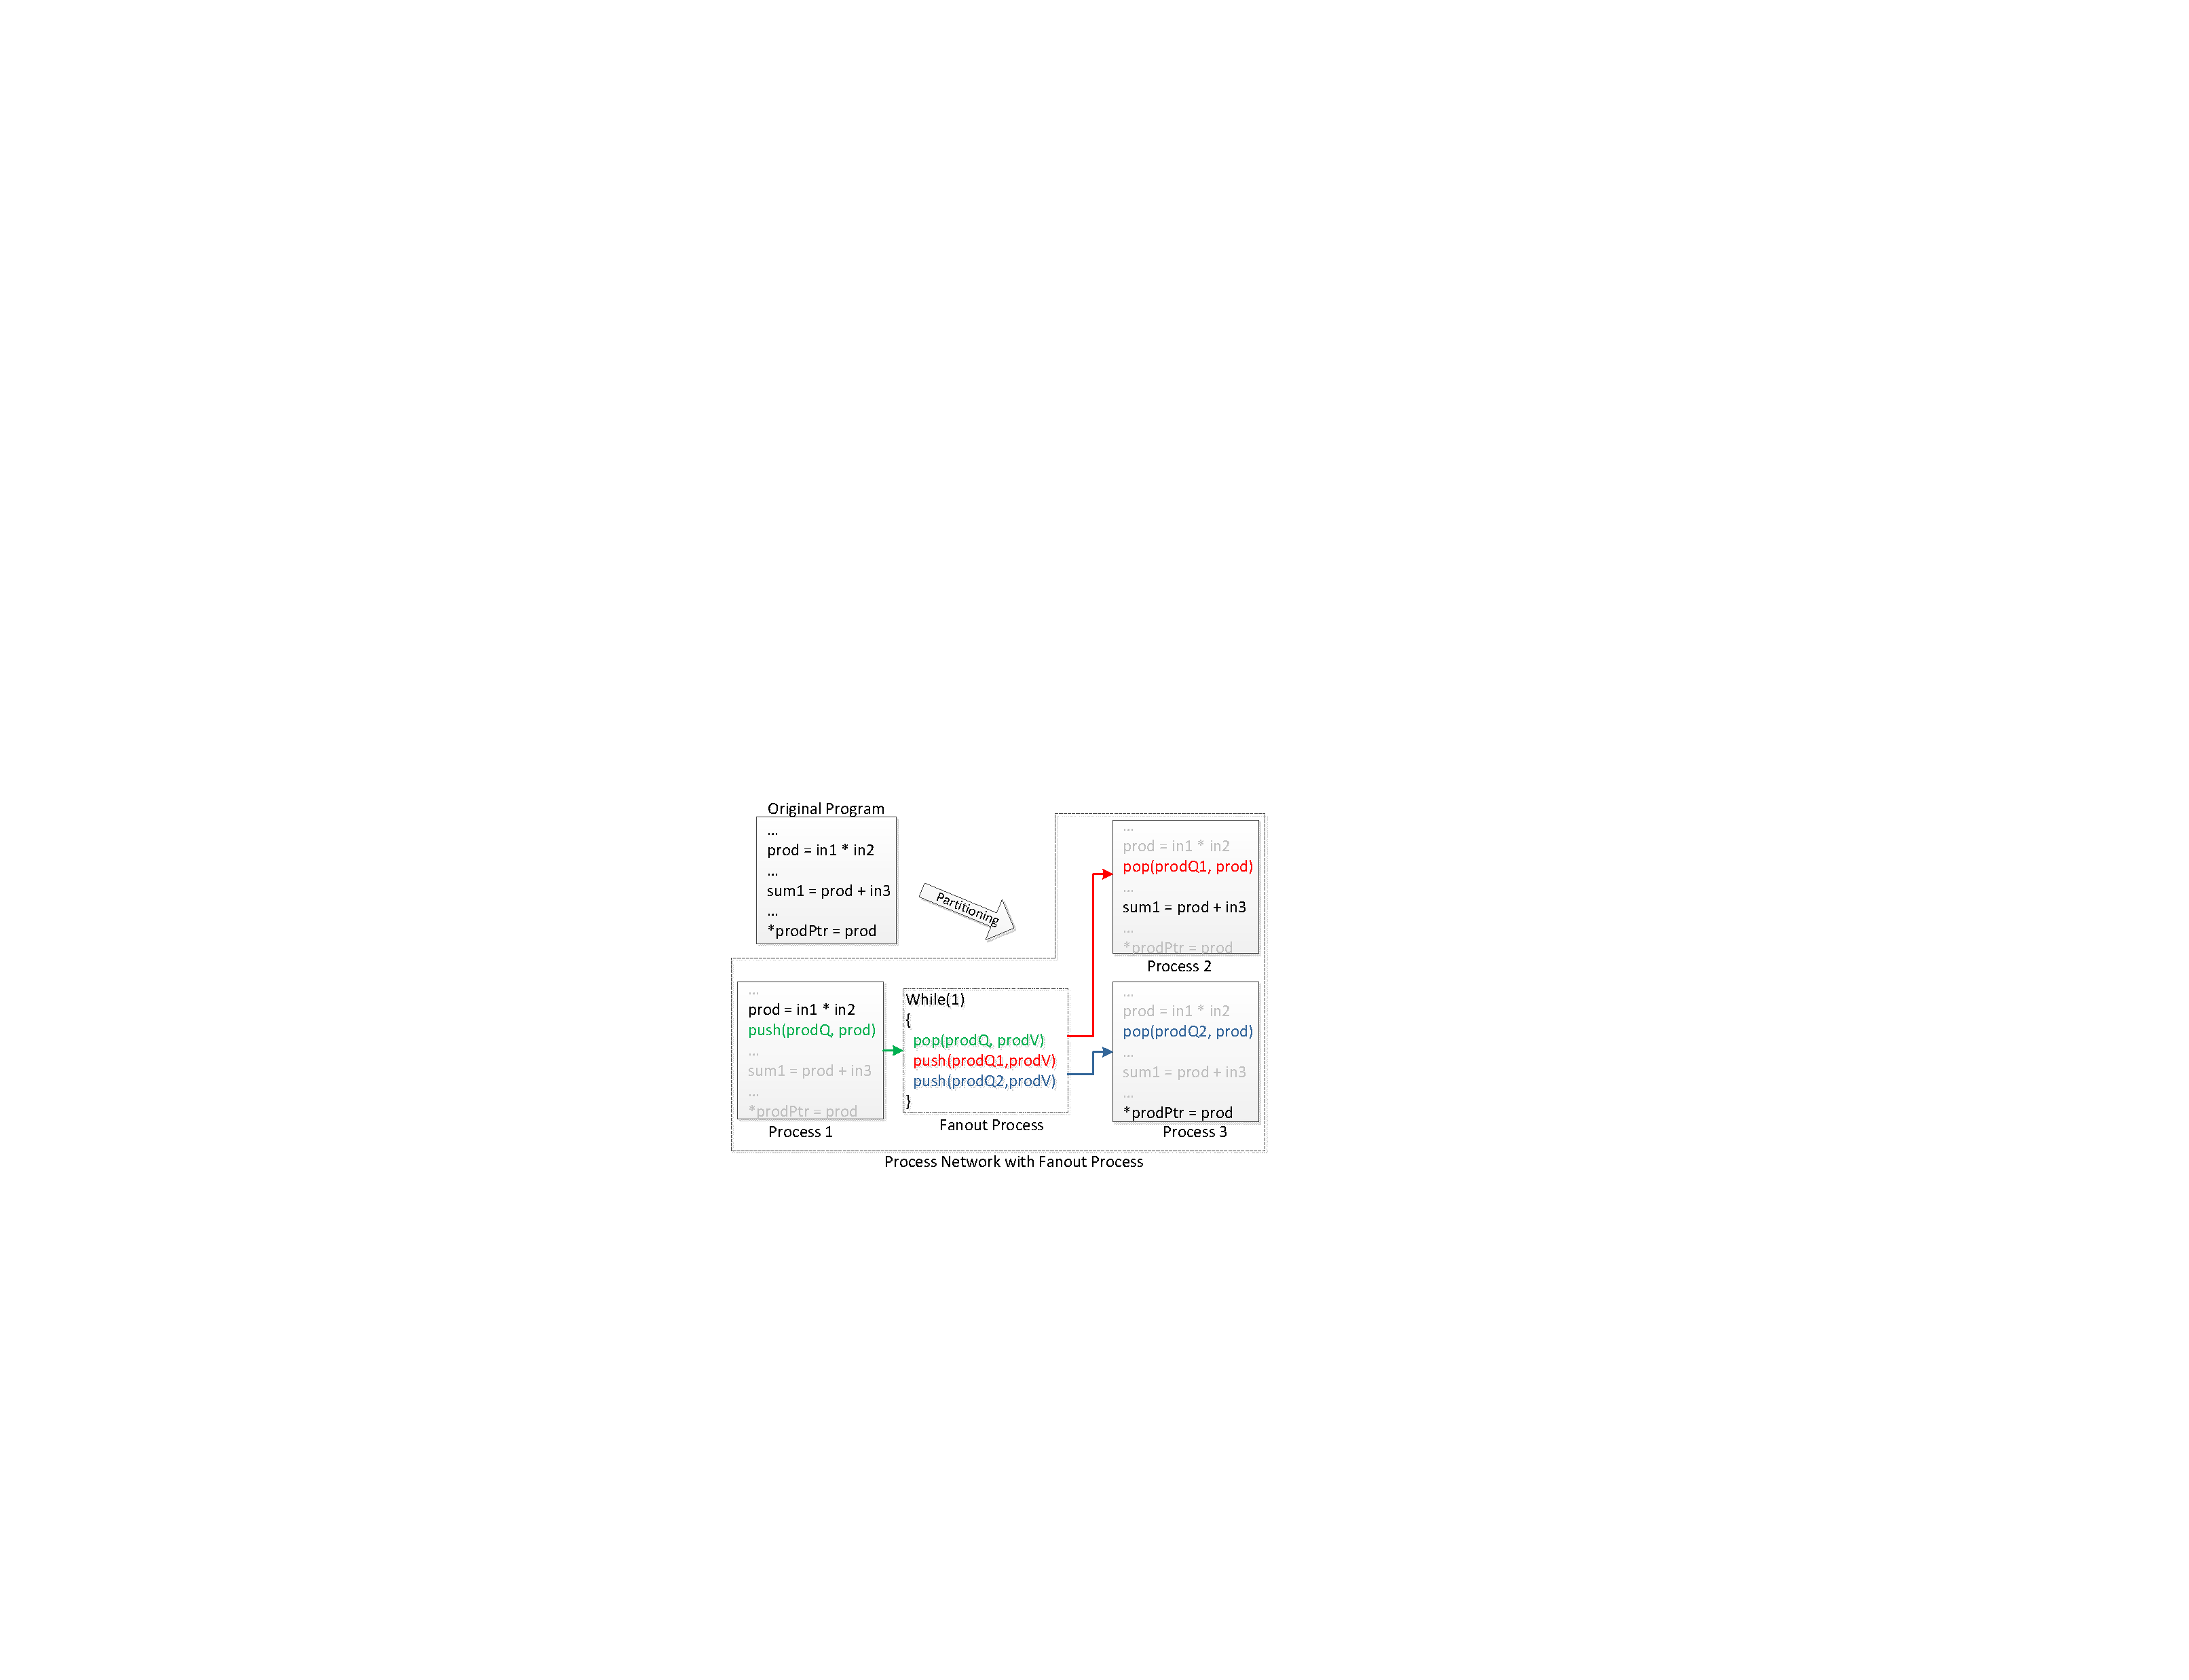
\includegraphics[width=0.65\linewidth]{chap4fig/fanout.pdf}
\caption{Addition of Fanout Process while Partitioning
\label{fig:fanout}}
\end{center}
\end{figure}



\section{Bounded Execution of the Process Network}
In real implementation of a KPN, 
it is impossible to have unbounded communication FIFOs between
processes. In~\cite{}, KPNs are 
categorized into strictly bounded, bounded and unbounded ones.
A KPN is strictly bounded if and only if any execution of of the network requires bounded space. It is bounded if and only if there are some
execution requiring bounded space while it is unbounded if and only if any
execution requires unbounded space. Methods to find bounds for communication channels
in KPNs were discussed in~\cite{}\cite{}. In general, whether a
KPN is bounded is undecidable~\cite{}, but for our process networks, which
are generated from sequential programs expressed in single static assignment
form, we can analyze the boundedness of the FIFO channels in various
scenarios. Note here we try to deduce properties applicable for
networks created by any arbitrary partitioning algorithms applied to
the original CDFG. Thus they also apply to the pipeline generated
using method outlined in chapter~\ref{decoupleChap}, which is just
one specific instance of all possible KPNs producible from a sequential program.


More specifically, given a sequential program $S$ in single static assignment form, we can partition the program into a process network $N$, consisted of a set of normal processes $P$, a set of fanout processes $F$, and a memory process $M$. 
Also, as mentioned in chapter~\ref{decoupleChap}, if an instruction is assigned to
$p$ and it is taking in tokens from instructions in other processes, a placeholder
instruction (and its owner basic block) is instantiated local to $p$, whose sole purpose is to receive
the actual token from the producer/fanout process. For $M$, it can be seen as containing a mirroring of all the memory accessing
instructions distributed among $P$, and each of its mirrored instructions 
produces tokens for the corresponding $p$ to consume.

\begin{definition}
Let $I$ be the set of instructions in the original $S$. For every $i \in I$, each
execution of $i$ is defined as a instruction instance $i_k$, where $k \in \Bbb{Z}$.
 In each $p \in P$, 
every instruction $j \in J^p$ corresponds to one $i$ in $S$, and every execution of this instruction $j_k$ corresponds to one $i_k$ in $S$. Let 
each of the placeholder/consumer instructions in $p$ be $\underline{j}$, and each instruction actually producing value to transmit be $\overline{j}$, every instance
of $\underline{j}$/$\overline{j}$ in the same process reads from/writes to the same FIFO channel. Note for each $\overline{j} \in J^p$,
there will be one or more  $\underline{j} \in J^{p'}$ where $p' \in P\setminus p$, and they are connected either directly or through $f_i \in F$. Also let the set of $\overline{j}$
 and $\underline{j}$ in $p$ be $\overline{J^p}$ and $\underline{J}^p$ respectively,
 we then have $\overline{J^p} \cup \underline{J}^p \subseteq J^p$ as some instructions may be strictly used locally.
\end{definition}



\begin{lemma}
\label{bounded}
Any instance of network $N$ is bounded with FIFO space required for each channel = 1.
\end{lemma}




To prove Lemma~\ref{bounded}, we can constructively create an execution schedule $H$
which does not overflow the FIFOs of size 1. This can be performed by following the original program order in $S$. 
Whenever a instruction instance $i_k$  of $i$ is executed in $S$, we find its corresponding set in $P$, these are instructions distributed among one or more processes.
For each element $j \in J^p, p \in P$ in this set:
\begin{itemize}
    \item If $j \not\in \overline{J^p} \cup \underline{J}^p$, we can just schedule $j_k$.
    \item If $j \in \overline{J^p}$, i.e. it is a ``producer" instruction, $j_k$ is scheduled and then the instructions in $f_i$ are scheduled (assuming there is fanout), followed by all the other ``consumer" instructions $j' \in \underline{J}^p', p' \in P\setminus p$.
    

%If $i_k^p \in \overline{I^p}$, the fanout process $f_i$, if there is any, is then scheduled. Subsequently, all the $\widetilde{i_k^p'}$ are scheduled.
    \item If $j_k$ accesses memory, then the instructions in the corresponding response block in $M$ is immediately scheduled to serve the request before everything else.
    \item If $j \in \underline{J}^p$, do not schedule it directly, wait for the producer instruction and $f_i$ to be scheduled.
\end{itemize}
Since the consumers of the tokens are always executed immediately after the producer instruction, the FIFOs will not see a backlog of tokens.

\begin{definition}
Let the schedule of instructions in each $p \in P \cup F$ be $G(p)$, we say $G(p)$ is locally consistent with $H$ if
and only if
$j'_x \prec j''_y$ in $H$ $\Rightarrow$ $j'_x \prec j''_y$ in $G(p)$
, $\forall j', j'' \in J^p$, 
$x, y \in \Bbb{Z}$. Additionally, if we have a schedule $H_s$ for a set of instruction instances  which can belong to different processes, we say $H_s$ is globally consistent with
$H$ if and only if $j'_x \prec j''_y$ in $H$ $\Rightarrow$ $j'_x \prec j''_y$ in $H_s$
 where  $x,y \in \Bbb{Z}, j' \in J^{p1}, j'' \in J^{p2}, p1 \in P \cup F, p2 \in P \cup F$.
\end{definition}


It should be apparent that if instances of a producer/consumer
instruction pair around a FIFO are globally consistent to $H$, we
do not need to have FIFOs with size greater one for our execution.
Meanwhile, as $H$ is derived from the original program order of
the sequential program $S$, all locally consistent schedules $G(p)$ 
do not violate data dependencies imposed by $S$.


\section{Artificial Deadlock in Process Network}
In actual implementation of KPN where FIFOs have fixed sizes, blocking
writes are introduced so that processes block when trying to write to a full FIFO.
This induces artificial deadlock as described in~\cite{}. 
When an artificial deadlock occurs, a circular dependency is formed among
processes, none of whom can make progress. At least one of the processes
in the cycle is blocked on write -- therefore the deadlock is ``artificially''
introduced by the size limit of FIFOs. 

Being a network of sequential processes and memory connected together by
bounded FIFOs, the computational pipeline synthesized may experience
artificial deadlocks as well. The interaction between the sizing of the FIFOs 
and the occurrence of deadlocks needs to be analyzed to ensure the liveness
of our pipeline.
\begin{comment}
\begin{lemma}
\label{blockingwriteconsistent}
In the presence of blocking writes, given a pair of instruction $\overline{j'} \in p1, \underline{j}'' \in p2$ writing to and reading from a FIFO, all their
instances are globally consistent with $H$ if the FIFO is of size one.
\end{lemma}

Lemma~\ref{blockingwriteconsistent} can be proven by contradiction.....
\end{comment}
\begin{lemma}
\label{nondeadlock}
Assuming requests to $M$ is first-come first-served,
all FIFOs are of size one and blocking write,
as long as $G(p), \forall p \in P \cup F$ are locally consistent with $H$,
artificial deadlock will not occur in $N$. 
\end{lemma}

Assume there is an artificial deadlock, we can go around the dependency
cycle and examine the blocked processes $P_b \subseteq P \cup F$. For a process $p_b$
to be blocked at instruction instance $j_k$, $j_k \in J^p$ is either reading from an empty
FIFO, or writing to a full FIFO. For the former case, the FIFO is empty because the producer of the token
$j'_k \in J^{p'}$ cannot execute, which indicates an earlier instruction 
instance $l_m$ in $G(p')$ is blocked. For the later case, the FIFO is full because the consumer $j''_{k-1} \in J^{p''}$ of the earlier token produced by
$j_{k-1}$ cannot execute, which also indicates an earlier instruction in $G(p'')$
is blocked. Apply this reasoning recursively around the circle of dependencies,
we have a chain of instructions instances $j_k \succ l_m \succ ... \succ j_k$
or $j_k \succ j''_{k-1} \succ ... \succ j_k$ in $H$, as each pair in the chain
comes from a schedule locally consistent with $H$. This chain is self-contradictory
and therefore the scenario for artificial deadlock can never occur. 

The memory subsystem, being FCFS, always produces tokens some processes are waiting to consume, there is no possibility of it being blocked on write, and thus being
part of the dependency cycle causing the deadlock.


As each $G(p), p \in P \cup F$ is locally consistent with $H$, which is derived from
the program order of the original $S$, we can conclude that if each of
the generated subgraph is executed strictly according to the original
program order, we will have a pipeline free from artificial deadlock. This
will guarantee, for instance, when processors are used as the execution substrate, the network will produce the correct result as
each process is executed according to program order. On the other hand, when
HLS is used to create hardware accelerators from them, this guarantee may not
hold anymore since aggressive parallelization and reordering of instructions
would violate the consistency between $G(p)$ and $S$. We thus need to examine
the  effect of instruction reordering on the liveness of our pipeline.



\begin{figure}[htp]
\begin{center}
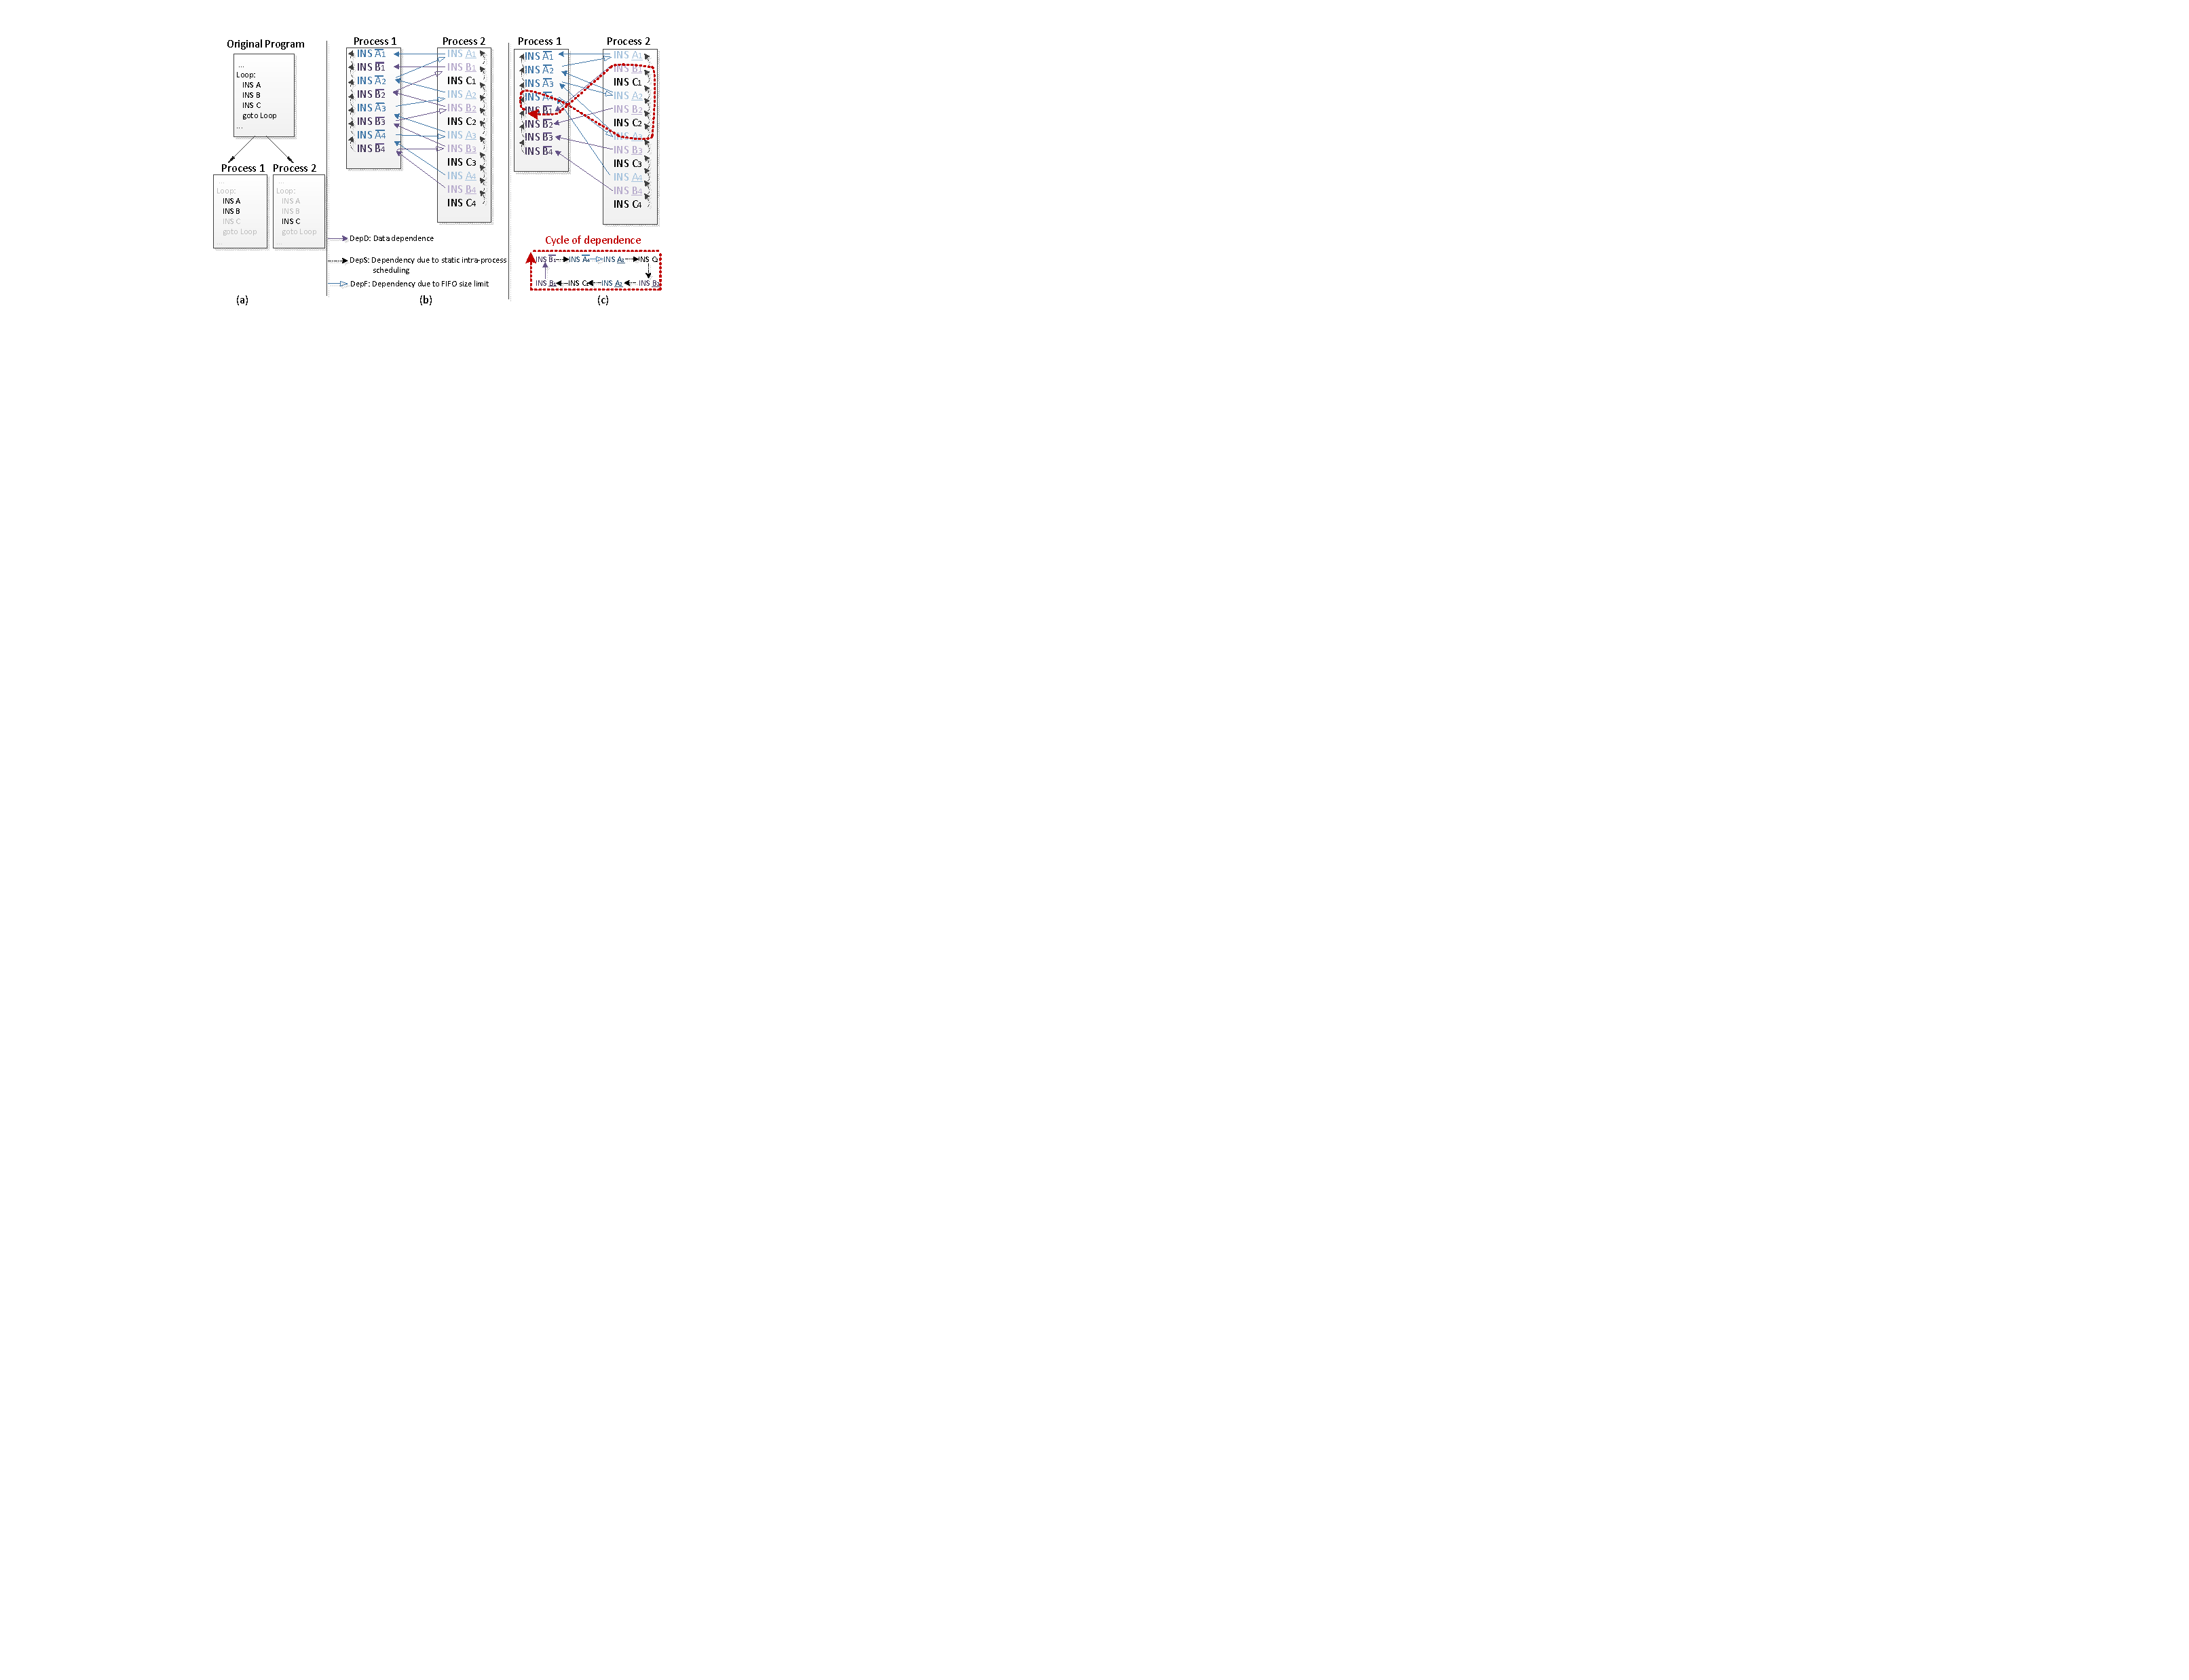
\includegraphics[width=1.0\linewidth]{chap4fig/cycleInstances.pdf}
\caption{a) partitioning of the original program into two processes; b) each process executes according to the program order; c) instructions in process 1 are reordered statically
\label{fig:deadlockfig}}
\end{center}
\end{figure}

\section{Liveness in HLS-generated Computational Pipeline }
Figure~\ref{fig:deadlockfig} shows a simple example of a otherwise deadlock free network becomes problematic
when the instructions are statically reordered in individual processes by HLS. 
Due to the size limit of the FIFOs, which is assumed to be one here, the execution
of the producer instruction is dependent on the completion of the previous instance
of the consumer instruction. In figure~\ref{fig:deadlockfig}(c), when the instructions in process 1 is statically reordered, a circular dependency is formed
between instructions: INS $\overline{B_1}$ cannot execute unless
INS $\overline{A_4}$ completes, and INS $\overline{A_4}$ cannot execute until
INS $\underline{A_3}$ consumes the token from INS $\overline{A_3}$. But INS $\underline{A_3}$ cannot happen until INS $\underline{B_1}$ occurs, and
that depends on the completion of INS $\overline{B_1}$.  An artificial deadlock
is therefore created. 

In this particular example, if the size of FIFO for $\text{INS }A$ is increased
from 1 to 3, then the execution of INS $\overline{A_4}$ would be dependent on 
INS $\underline{A_1}$ instead of INS $\underline{A_3}$. The
channel can now buffer the tokens produced by INS $\overline{A_1}$ -- INS $\overline{A_3}$ before INS $\underline{A_1}$ needs to be invoked to create empty slot. With this increase in buffer space, the cycle of dependence is broken as there will be no path of dependence from INS $\underline{A_1}$
to INS $\overline{B_1}$. The deadlock no longer exists.


Indeed, this is the classic approach in resolving artificial deadlock~\cite{}. 
When artificial deadlock is detected, the process which is write blocked is found, the full FIFO it tries to write to is given more capacity. 
However, in a network implemented in hardware, the FIFO size cannot be easily increased.
%As the producer and consumer instruction instances are rescheduled differently with
%respect to other instructions in their own process, blocking write causes
%artificial deadlock. Increasing the number of slots in the FIFO can help resolve
%this problem. 
To determine the needed buffer space in the channels \textit{a priori}, simulations are sometimes used~\cite{}. It relies 
on using representative dataset as input and for certain type of problems, simulation results may not provide any guarantee, especially if the control flow is runtime data dependent. In this section, we want to analyze the interaction between FIFO
sizing and intra-process instruction scheduling, 
so we can better understand
their joint effect on the liveness of the process network. 
%what kind of reordering can be permitted and its effect on the FIFO space needed.
\begin{comment}
We have proven that when each $p \in P$ execute according to the original
problem order, no artificial deadlock would occur even when the FIFO is of size one.
Our example shows that when producer (or consumer) instructions are rescheduled with respect to other instructions in their own process, more tokens may
need to be buffered before the consumer instruction is activated. To ensure progress
of the network, we need to size the FIFOs such that a
consumer instruction instance is always scheduled before the cycle of blocked
processes is formed.
\end{comment}
\subsection{Artificial Deadlock Detection without Simulation}
In our networks derived from sequential programs, given each process' schedule and each FIFO's size, it is possible
to find out if a potential artificial deadlock can arise without running simulation. As demonstrated in figure~\ref{fig:deadlockfig}, we can add $DepS$ edges between instruction instances belonging to the same process, and $DepF$ edges between
producer/consumer instruction instances writing/reading from the same FIFO.
Note for a FIFO of size $s$, $DepF$ edges are added between $\overline{j_k}$ and $\underline{j_{k-s}}$ to indicate that the producer instruction instance is disabled
until the consumer instruction instance is invoked. The graph thus obtained
can be checked for cycles, which indicate the occurrence of artificial deadlock.


The schedule for each process may contain potentially infinite instruction instances, resulting in a graph with infinite number of nodes,
which makes it impossible to guarantee the absence of artificial deadlock.
However, when we use HLS tool to map each process,
a short, repeatable schedule is generated and we can represent the
dependencies between instruction instances using a manageable
sized graph. 
%Meanwhile, we
%can take advantage of the transitive property of dependencies 
%to reduce the number of edges in the graph as well. 
Figure~\ref{fig:singlelevelLoopCylce} shows a more concise
representation of the schedule we have in figure~\ref{fig:deadlockfig}(c).
Various dependency edges are associated with weights to 
represent the difference between the subscripts of the pair of instruction
instances. For instance, as INS $\overline{A_4}$ is 
scheduled before INS $\overline{B_1}$ in process 1, the edge from INS $\overline{B}$ to INS $\overline{A}$ carries
a weight of 3, meaning the occurrence of INS $\overline{B_x}$ depends on the completion of INS $\overline{A_{x+3}}$. Similarly, when the channel between 
INS $\overline{A}$ in process 1 and INS $\underline{A}$ in process 2 are of size one, INS $\overline{A_x}$ depends on the completion of INS $\underline{A_{x-1}}$, 
which is represented by the $-1$ weight of the edge representing this
dependency. The edges denoting data dependencies between processes
are always of weight 0, as each pair of the end points represents the same instruction instance, with one being the actual source of the data, and the other a placeholder in the consumer process.
Note the weights assigned correspond to the largest differences
in instance subscripts, representing the furthest an instruction is running
ahead of its dependents. In the presence of branches, it is possible that
an instruction does not get executed every loop iteration. The subscripts
assumed by the instruction instances do not take this into account, i.e. $I_3$
in iteration 3 despite it is actually the second time $I$ is executed. Thus under
this particular scheme, the subscripts assigned to instruction instances
are just the iteration numbers of the enclosing loop in the original program.
Note in the literature about loop dependency analysis~\cite{Kennedy:2001:OCM:502981}, the term iteration number is generally associated with analyzable loop index, with
bounds and regular change steps. Here, however, we just use the term to represent the simple ordering of iterations, with or without actual loop indices.

To shrink the size of the graph, we have taken advantage of the transitive property of dependencies to reduce the number of the $DepS$ edges in the graph.
As only the scheduling of producer/consumer instructions matters for
deadlock detection, we can further trim the graph by omitting any $DepS$ edges having end point $j \not\in \bar{J^p} \cup \underline{J}^p$. In figure~\ref{fig:singlelevelLoopCylce}, for instance, the $DepS$ from INS $\underline{A}$ to INS $C$ can be redirected to INS $\underline{B}$, accompanied by the deletion of INS $C$ and the $DepS$ edge from INS $C$ to INS $\underline{B}$.


\begin{figure}[htp]
\begin{center}
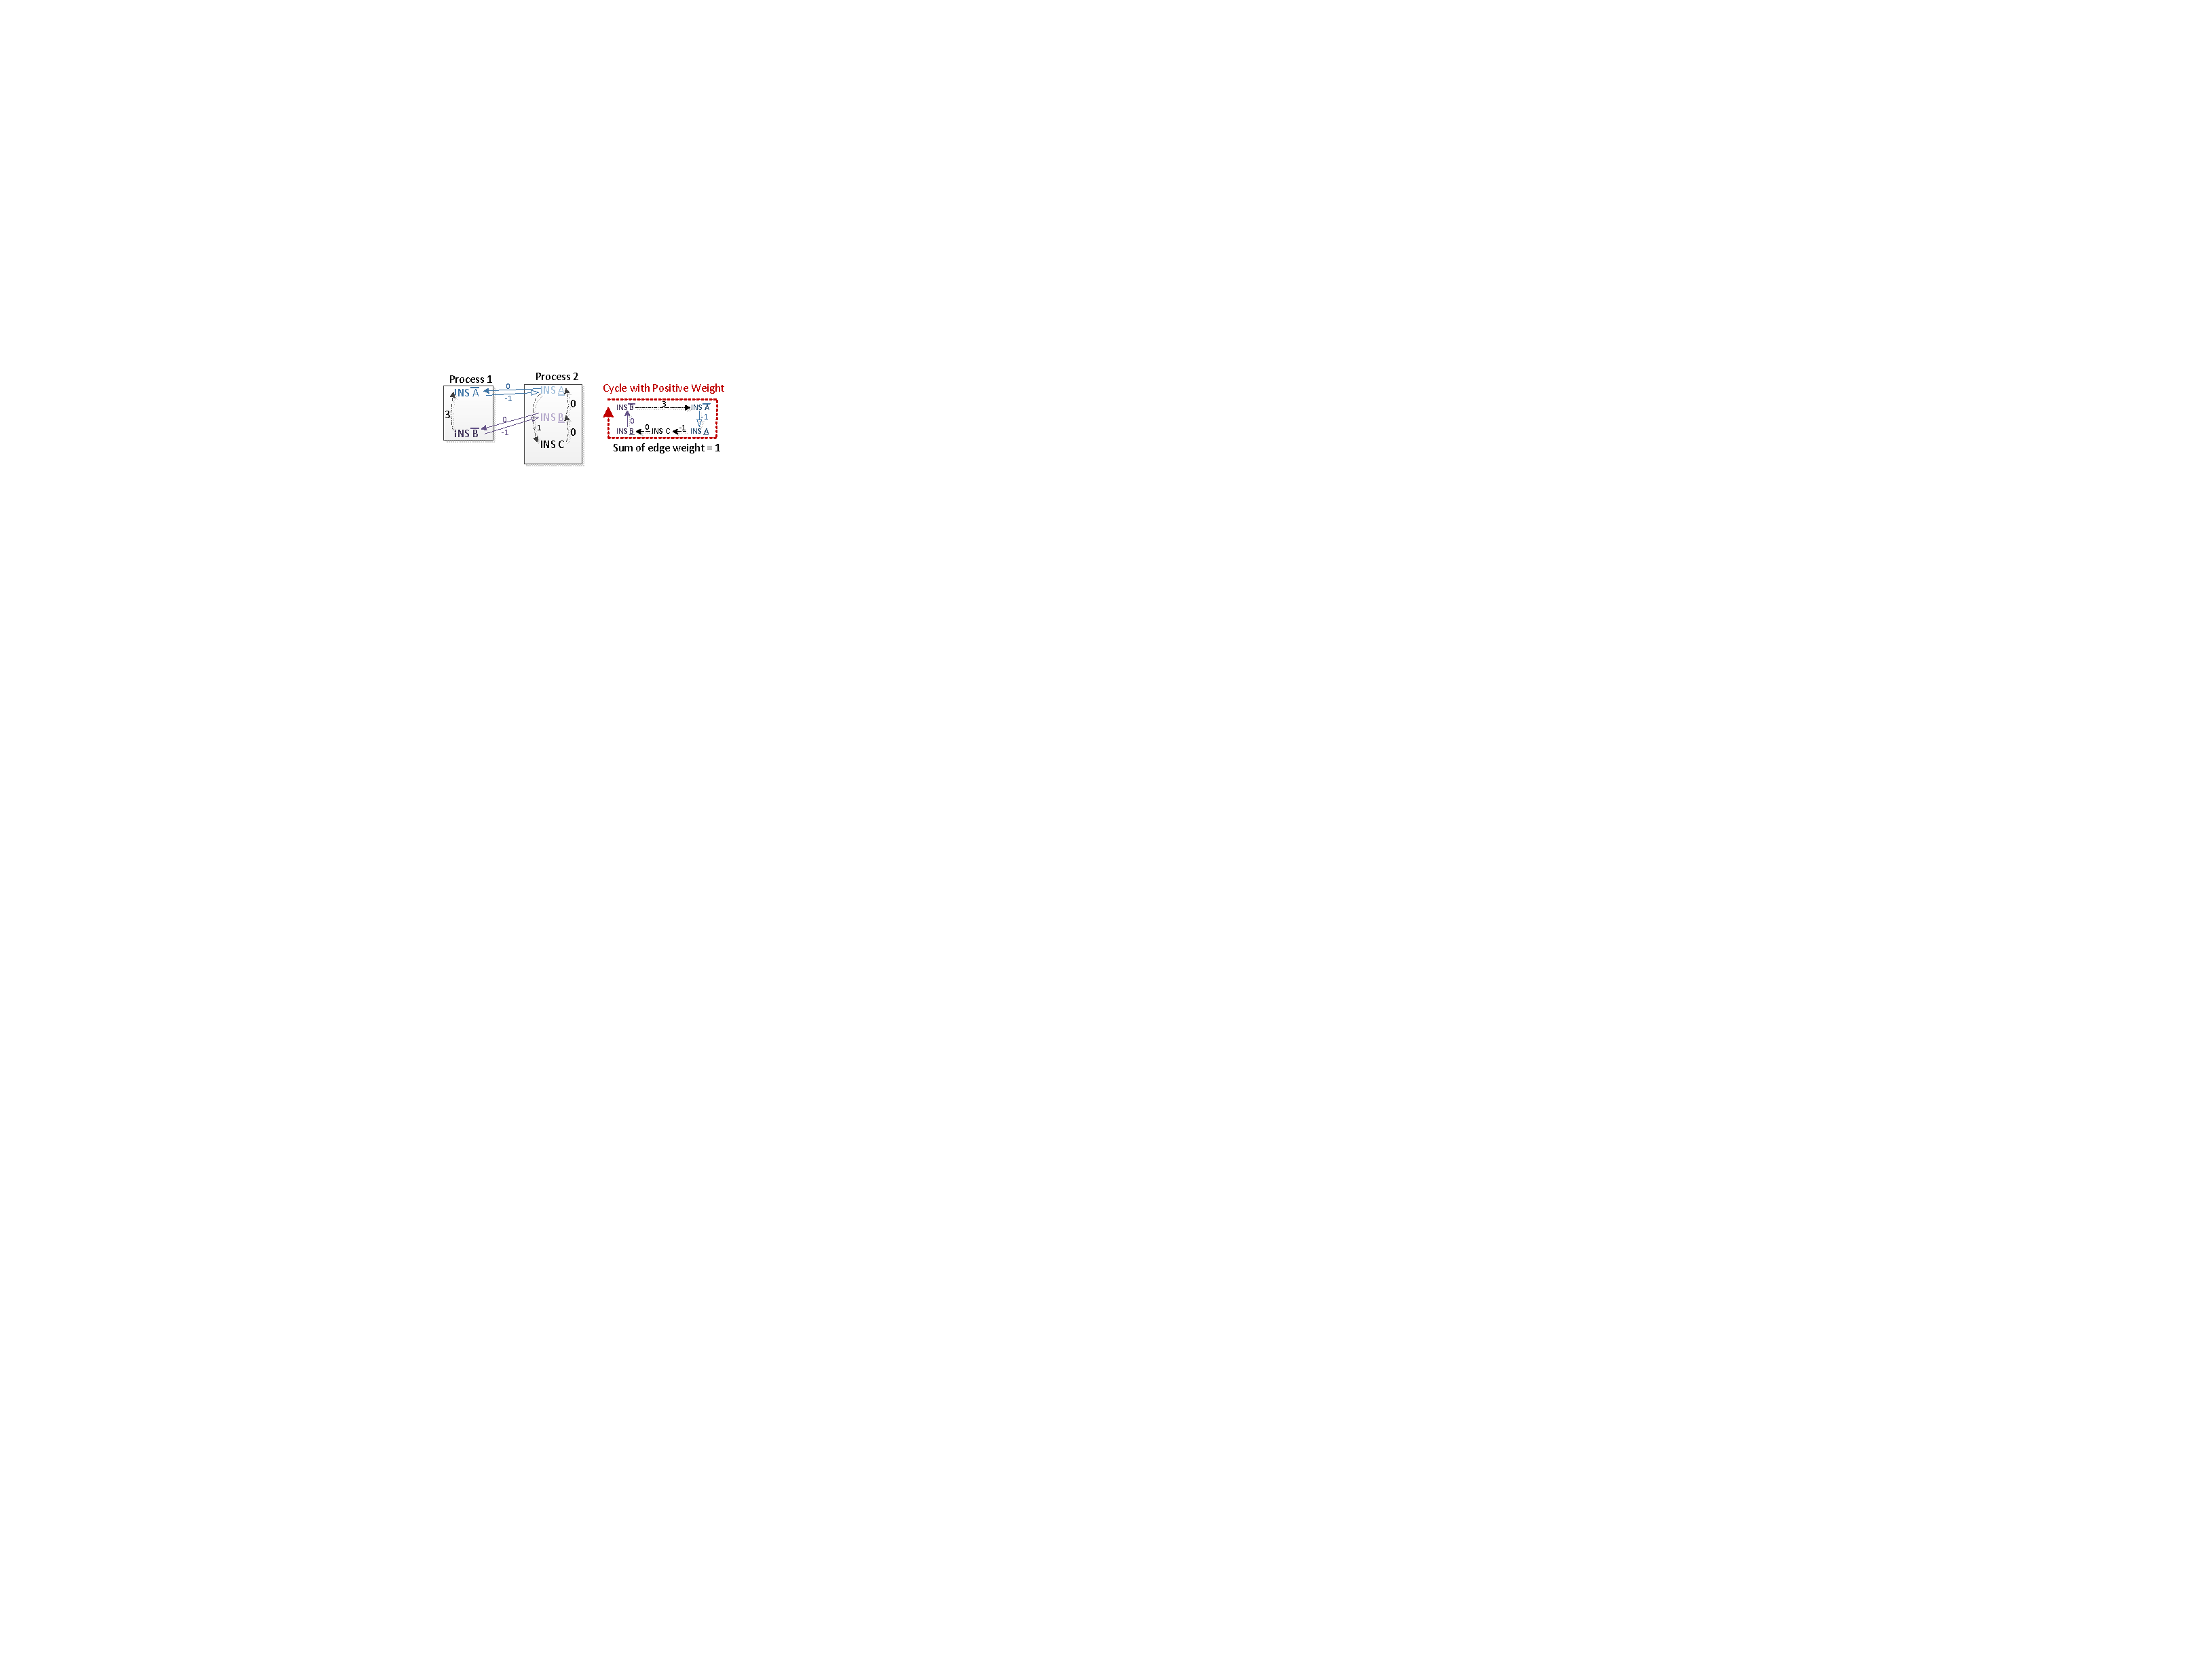
\includegraphics[width=0.7\linewidth]{chap4fig/singlelevelLoopCycle.pdf}
\caption{Deadlock Detection using Graph with Weighted Edge
\label{fig:singlelevelLoopCylce}}
\end{center}
\end{figure}

Now, if a non-negatively weighted cycle is found within this graph, we have an artificial deadlock.
A cycle in the graph means we have an instruction instance $I_x$, whose occurrence depends on the completion of $I_{x+w}$, $w$ being the weight of the cycle.
With $w$ being greater or equal to zero, $I_x$ cannot happen until itself or a later instance happens -- we have a deadlock. 
The computation to find deadlocks may potentially be expensive. In the worst case, the number
of simple cycles in the graph can be exponential in
$|V|$, the number of nodes in the graph. Practically however, the number of
nodes involved are approximately the same as the number of channels needed, while the graph is rather sparse in the connectivity between these nodes. 
Methods such as~\cite{doi:10.1137/0204007} can be used for efficient
enumeration of the cycles and the subsequent identification of the deadlocks.



Resolving
the deadlock involves choosing one of the $DepF$ edges
in the cycle and add enough slots (making the weight more negative)
such that the sum of the edge weights becomes negative. For
one particular cycle, the $DepF$ edge whose channel has the smallest width can be selected, as this minimizes the cost of adding the extra slots. However,
as multiple non-negatively weighted cycles can be present simultaneously,
the global optimal solution would involve finding a set of $DepF$ edges, 
and minimize the aggregate cost of incrementing each for all cycles to be resolved, which 
is NP-Hard. (maybe I shall formulate an ILP here??)
\begin{figure}[htp]
\begin{center}
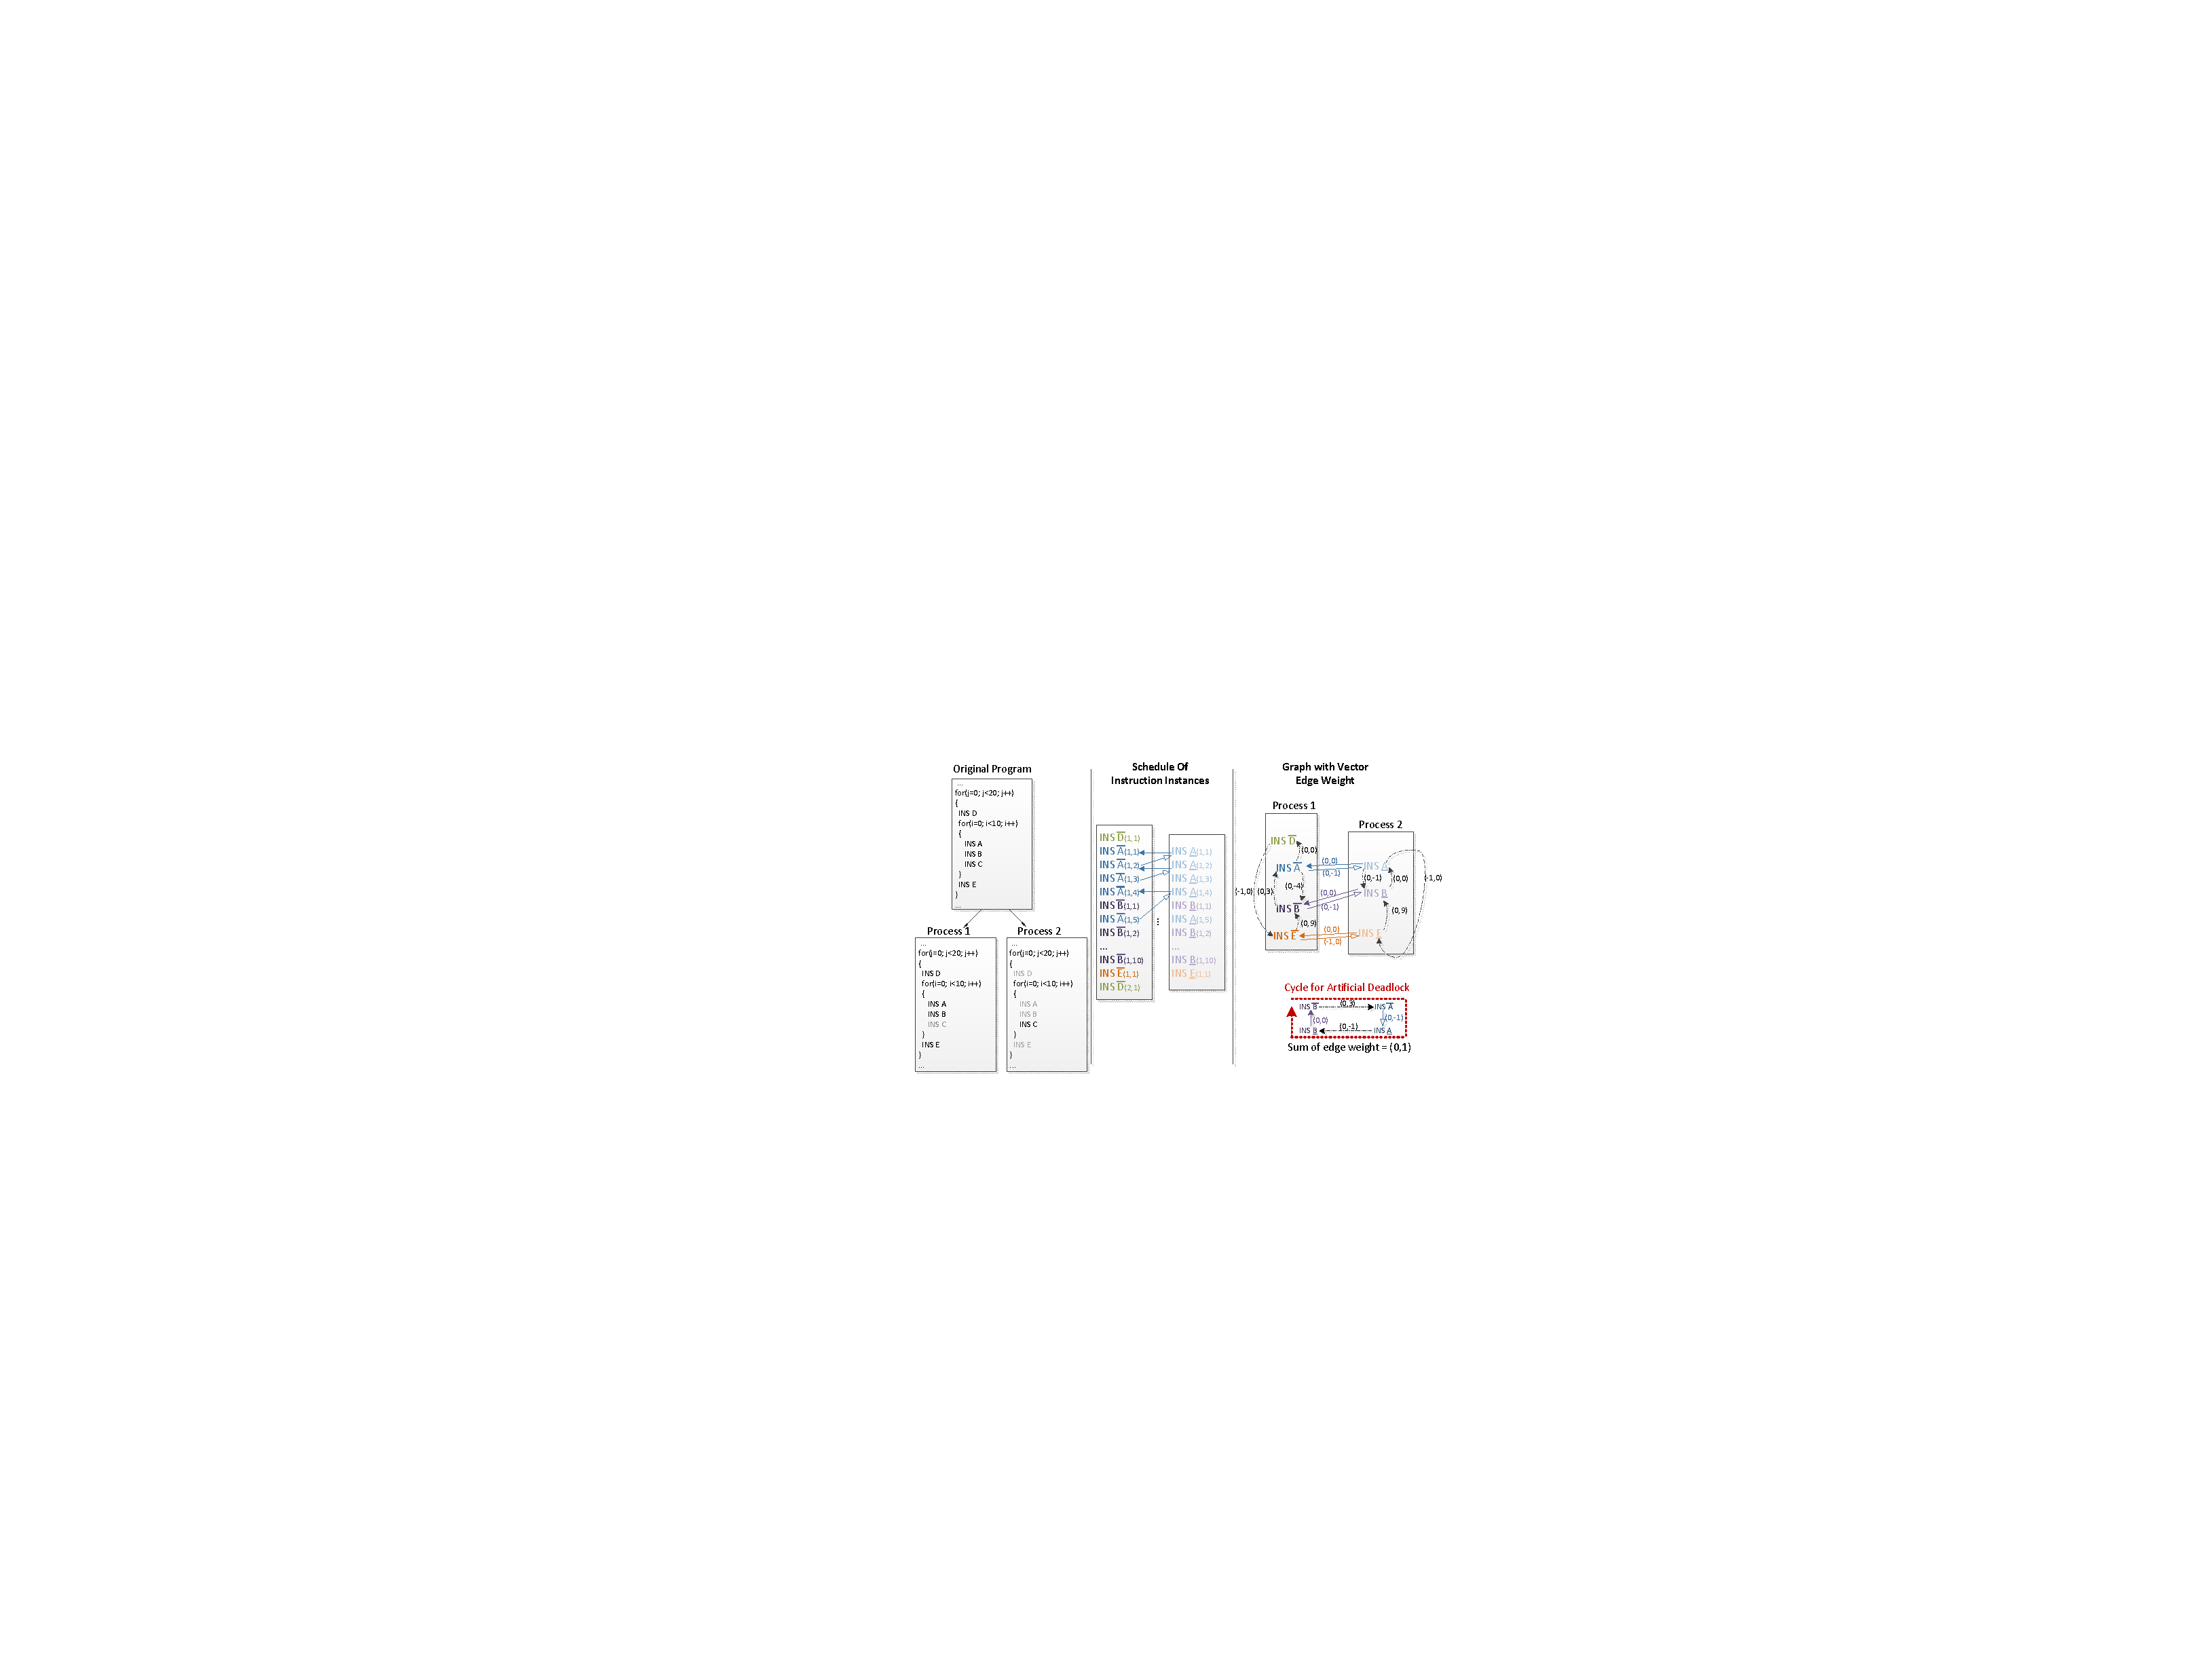
\includegraphics[width=1.0\linewidth]{chap4fig/vectorAnnot.pdf}
\caption{Multi-level Loop Nest Deadlock Detection
\label{fig:vectorannot}}
\end{center}
\end{figure}

So far we have formulated a method for deadlock detection and resolution
for a single level loop. To generalize this method for loop nests of multiple
levels, we associate each instruction instance with
a vector of iteration numbers, with the earlier elements corresponding to the outer loops.
%indicating its position in the iteration space.
Subsequently, for the weight assigned to each of the edges, instead of
a single number, a vector is used. The number of elements in the vector
corresponds to the number of levels in the loop nest.
An example of this is shown in figure~\ref{fig:vectorannot}. 



All the vector weights assigned to the edges between instructions of
the same level in the loop nest are really the same as in the single level loop
example, except the padding of zeros to match the dimension of the iteration space. A more interesting case is the $DepS$ edge from INS $\overline{E}$ to INS $\overline{B}$, which goes from an outer loop instruction to an inner loop instruction. 
The last components of the subscript vectors of INS $\overline{E}$ instances are always 1
as the instruction does not execute in the innermost loop. The subscript vectors of INS $\overline{B}$ instances, however, can take a value up to 10 for its right most element, as the inner most loop has an iteration count of 10. Thus the weight $(0,9)$
means the $1$st INS $\overline{E}$ instance is scheduled after the $10$th occurrence of INS $\overline{B}$ in the current iteration of the outer loop.

In this modified graph, 
every cycles in the graph now has a weight sum which is also a vector. 
An deadlock is manifested as a cycle with weight being the zero vector ($\vec{0}$)
or vectors whose first non-zero elements (leading elements) are positive.
Similar to the case when we have scalar
weights, these weight vectors 
indicate an instruction instance depending on itself or a later instance in the iteration space, and thus a deadlock. The deadlocks can also be
resolved by finding the $DepF$ edges, whose change of capacity makes
all the cycles' weights' to have negative  leading element. 


\begin{definition}
When an artificial deadlock occurs, a cycle of dependency between instruction instances is formed. Define this cycle as $C_v$. Each instruction instance in $C_v$ corresponds to one instruction in the weighted graph. Define the cycle formed in the weighted graph by the corresponding instructions as $C_V$, and the set of instructions
as $V$. 
\end{definition}

As mentioned before, non-communicating instructions/instruction instances can be omitted in the graph without affecting the deadlock analysis, thus $V \subseteq \bar{J^p} \cup \underline{J}^p$. As the nodes in $C_v$ are instantiations of nodes in $C_V$, the edges in $C_v$ are also
instantiations of edges in $C_V$. Let these edges in $C_v$ carry the same weights as the $C_V$ edges they instantiate.

\begin{lemma}
\label{deadlock2cycle}
If there is an artificial deadlock in the network, there will be a cycle in
the weighted graph whose sum of edges
is either $\vec{0}$ or vectors with positive leading element. 
\end{lemma}

% we wanna prove the sum of edges in C_i is smaller than C_I
%Assume $C_I$'s weight has negative left most non-zero element, 
We can take any point in  $C_v$, and go around the
cycle $C_v$ to get a sequence $V^1_{X1}$, $V^2_{X2}$ ... $V^n_{Xn}$ where $V^1 ... V^n \in V$, $V^1 = V^n$ and $X_1 = X_n = X_1 + (X_2-X_1) + (X_3-X_2) ... (X_n - X_{n-1})$. The sum of edges in $C_v$ = $(X_2-X_1) + (X_3-X_2) ... (X_n - X_{n-1})$ =$\vec{0}$ as $X_1 = X_n$.  

If no two elements in $C_v$ map to the same
element in $V$, then the sum of edges in $C_v$ is equivalent to the 
sum of edges in $C_V$, which would be zero -- we have a cycle in the weighted
graph whose sum of edges is the $\vec{0}$.

Otherwise, we can have $C_v$ containing two instruction instances $U_{Y1}, U_{Y2}$ mapping to the same element $U \in V$, and instruction instances on the path between $U_{Y1}, U_{Y2}$ are all unique instances of instructions in  $W_1 \subseteq  V \setminus U$.  
Now we can construct a cycle $C_{W1}$ of instructions using $W_1$, and the weight of this cycle is the same as the weight of the path from $U_{Y1}$ and 
$U_{Y2}$ as every edge in the path is a unique instantiations of a corresponding edge in $C_{W1}$. This decomposition can be applied recursively to 
the remaining part of $C_v$ until we have $C_{W1}, C_{W2}...C_{Wn}$ whose
sum equals to the weight of $C_v$. Since weight of $C_v$ is  $\vec{0}$, 
they can either all be of weight $\vec{0}$, or at least one of them will have
positive leading element. This process is illustrated in figure~\ref{fig:decomp} for a single level loop.

\begin{figure}[htp]
\begin{center}
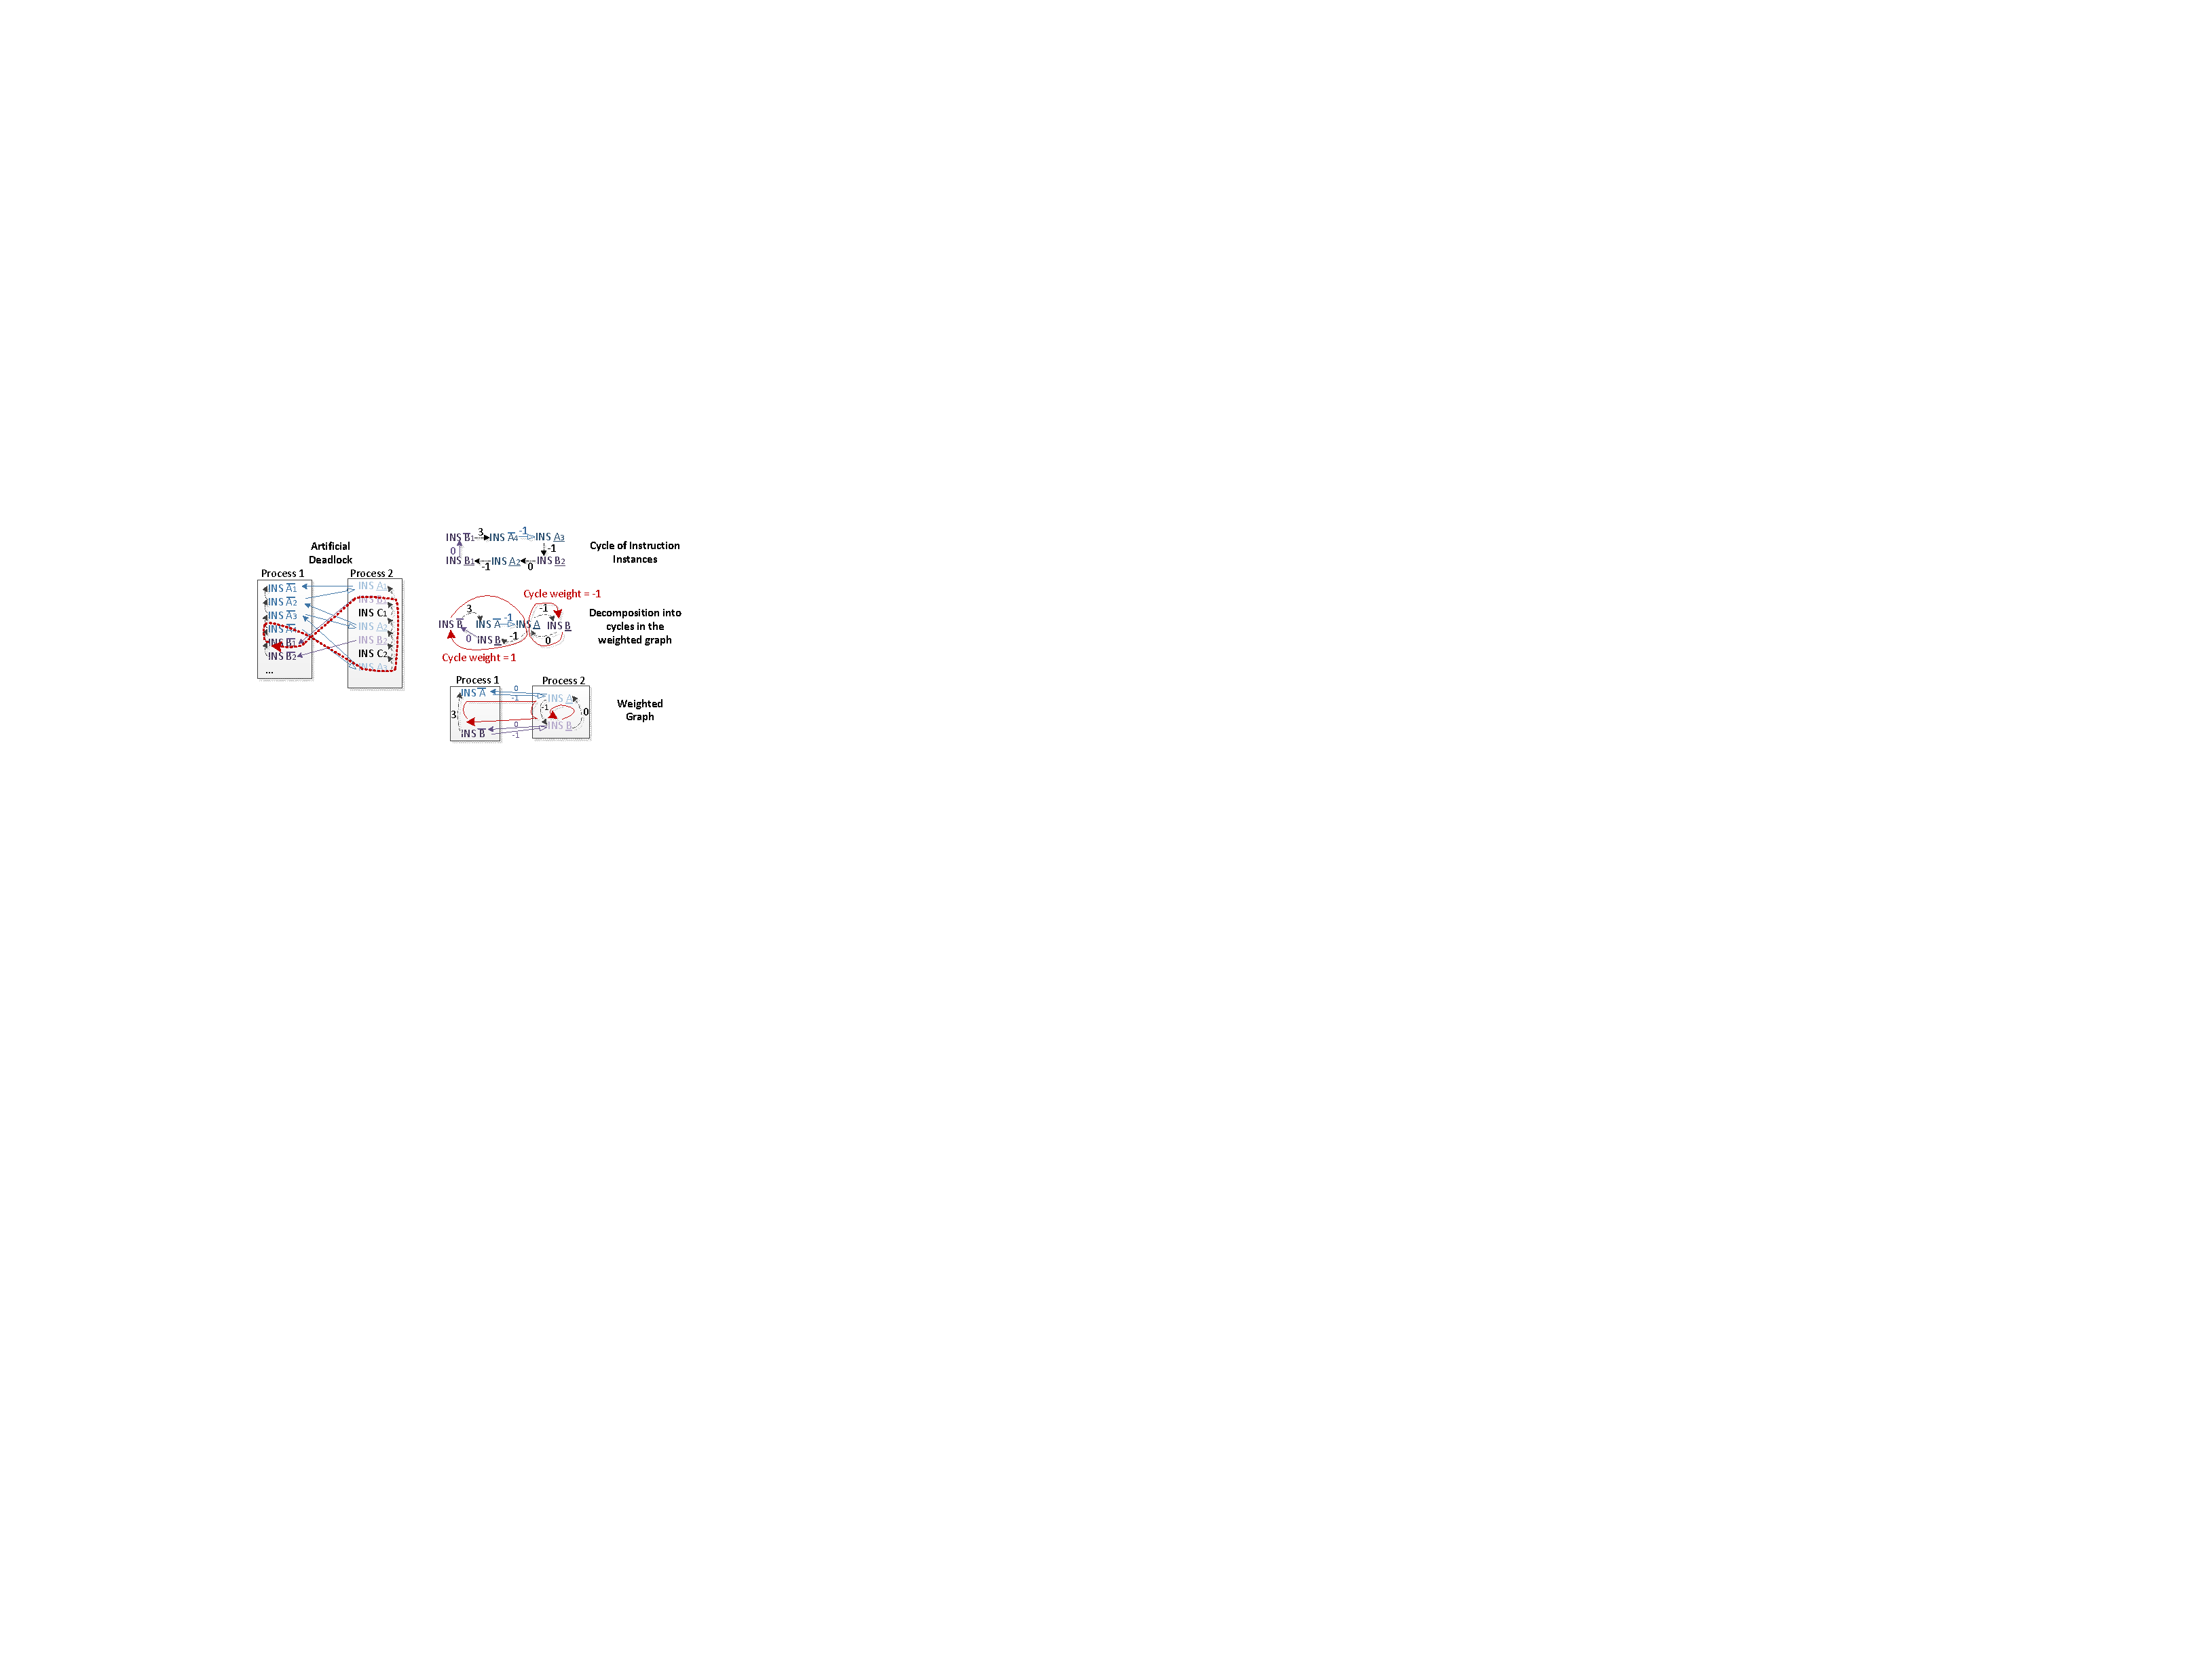
\includegraphics[width=0.9\linewidth]{chap4fig/decomp.pdf}
\caption{Decomposition of Cycle of Instruction Instances 
\label{fig:decomp}}
\end{center}
\end{figure}



As lemma~\ref{deadlock2cycle} is proven to be true, the absence of cycles of
weight $\vec{0}$ or with positive leading elements guarantees the the absence of artificial deadlock (the contrapositive).

\begin{comment}
In addition, the number of $DepS$ edges added can also
be reduced. Only the scheduling of producer/consumer instructions matters for
deadlock detection, therefore any $DepS$ edges having end point $j \not\in \bar{J^p} \cup \underline{J}^p$ can be omitted.For
the experiments we performed in chapter~\ref{decoupleChap}, we extract the
schedule from the HLS report and with FIFO size set to 64, no
potential deadlocks are detected.

With the detection mechanism in place, we can try to resolve the found deadlock by
increasing the FIFO capacity. In the case of using simulations for deadlock detection, there is always one FIFO whose capacity needs to be increased when a deadlock occurs. 
In our approach, however, if multiple $DepF$ edges are present in the cycle,
it's not immediately apparent which FIFO should be modified. There can also be
multiple cycles sharing some of the $DepF$ edges, 

there is a difference from the cases when simulation was used,
it may.  
\end{comment}



\begin{comment}

\begin{figure}[htp]
\begin{center}
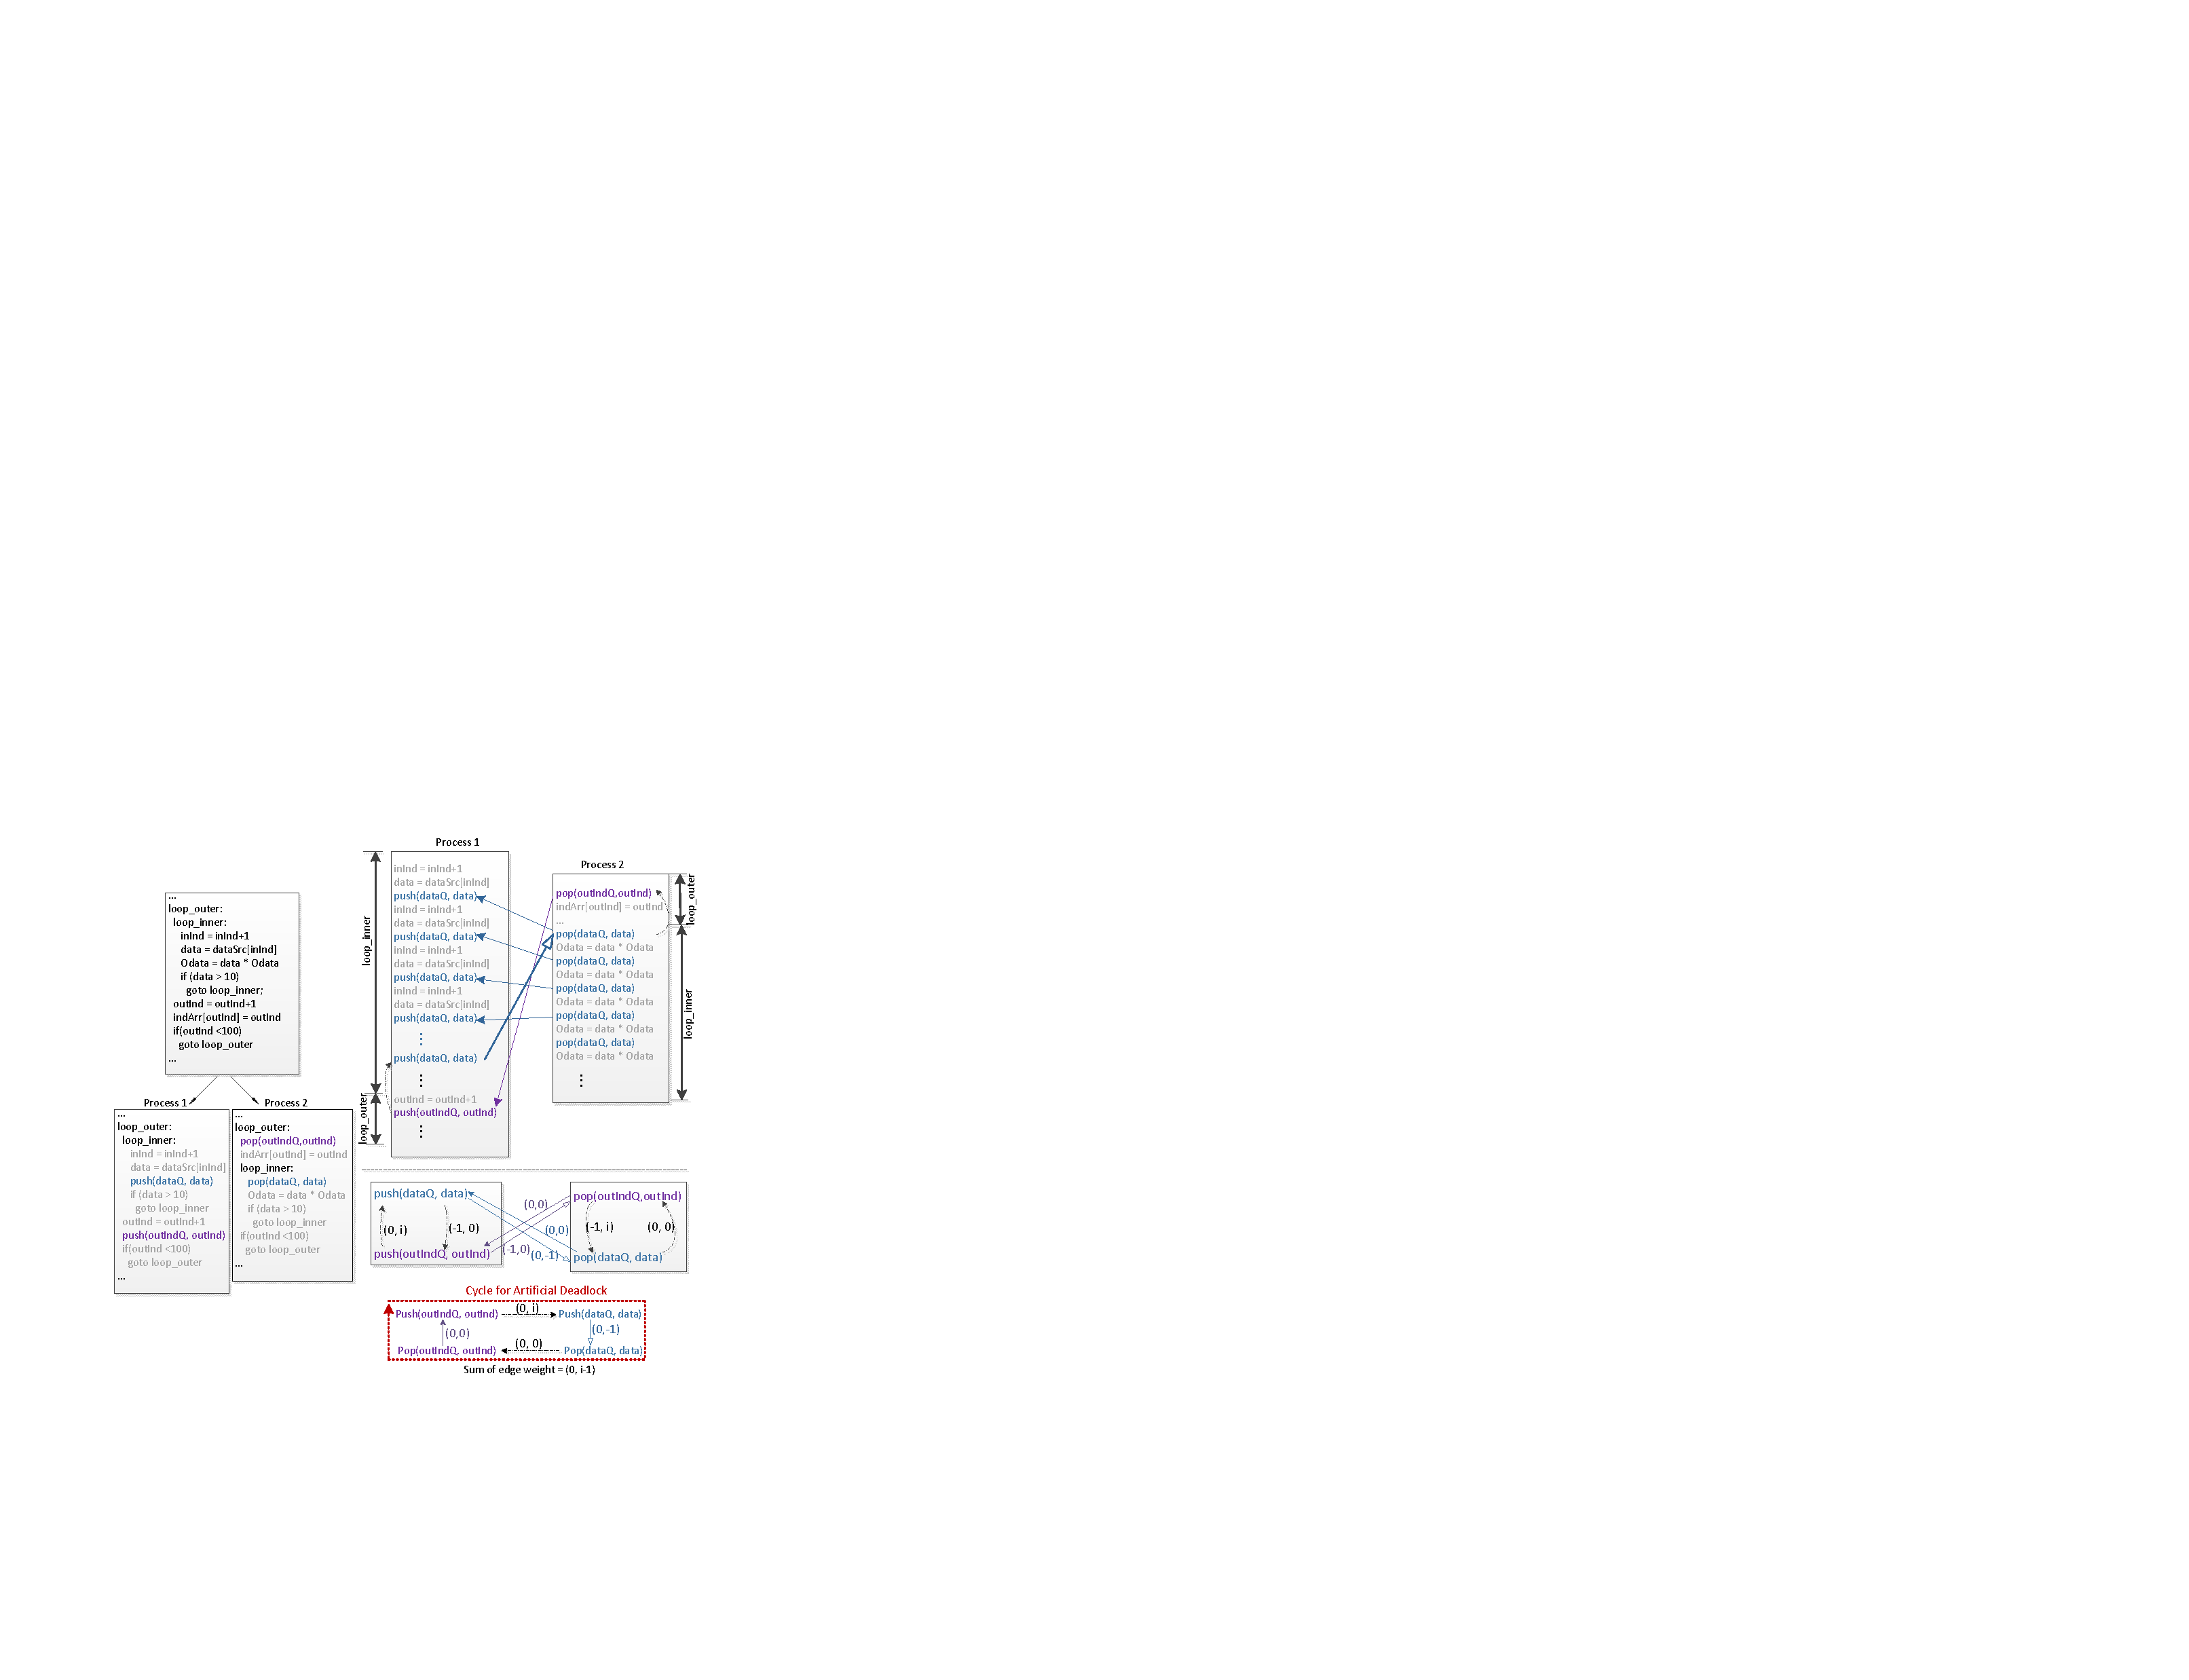
\includegraphics[width=1.1\linewidth]{chap4fig/unresolve.pdf}
\caption{Rescheduling Creates Statically Unresolvable Deadlock
\label{fig:badsitu}}
\end{center}
\end{figure}

\subsection{Statically Unresolvable Artificial Deadlocks}
Using the analysis framework we have formulated, we can construct situations
where artificial deadlocks may always occur, regardless of how much
space is statically assigned to a FIFO channel. Figure~\ref{fig:badsitu}
shows one example where no guarantee of deadlock freedom can be
statically obtained. 
Here, the outer loop consumer instruction
are rescheduled to before the start of the inner loop, while the corresponding producer instruction
executes after the completion of the inner loop iterations. As the
number of iterations of the inner loop is statically unknown, there will
always be a $DepF$ between a pair of the $push$ and $pop$ instruction instances (and therefore a cycle of dependence),
regardless of how large the FIFO size is. 

In the weighted edge graph, the size of the iteration space is represented
symbolically and the $DepS$ edge between the outer loop and inner loop producers carries a weight of $(0,i)$. Assuming FIFOs of size 1, a cycle of weight $(0, i-1)$ is found. Without knowing the bound of $i$, there is no way we can add enough
space to the $DepF$ edge between the producer and consumer of ``data" such
that the cycle weight has negative leading element.


The actual computation is shown
in this example to demonstrate the validity of the reordering. There is no local data dependency violated, yet artificial deadlocks are created in the network.
To prevent this type of unresolvable deadlocks, we can impose constraints on the
reordering of instructions performed by the HLS tools. The starting point of
instruction rescheduling is always the original program order, or more specifically the locally consistent $G(p)$. In the weighted graph representing the network of processes each scheduled according to $G(p)$, $DepS$ edges going from an instruction to its predecessor in the inner most loop all have weight $\vec{0}$. The weight of a $DepS$ edge from an outer loop instruction towards a preceding inner loop instruction has its leading element equals to the max number of inner loop iterations minus 1.
On the other hand,
The $DepS$ edge pointing to successors always has element -1 at 
the position of the vector corresponding to the outermost loop level among
the two instructions. 

In order to avoid creating unresolvable deadlocks,
we shall disallow any reordering creating cycles whose weight has non-statically
known leading elements. This can happen in two ways: 1) a statically unknown symbol
is added to the leading element of a cycle or 2) a new leading element is exposed
because the original one becomes zero. To prevent these scenarios, we can constrain changes at every edge. More specifically, 
rescheduling of instruction with respect to another instruction at the same level in the loop nest has additive effect on the edge weight. The extent
of rescheduling in HLS, however, is in general known statically, so it  



We have already proven that when all processes are scheduled  according to $G(p)$, there will be no artificial deadlocks, let alone unresolvable artificial
deadlocks. This does not mean there can be no cycles with zero 
Any reordering which causes a statically unknown number to become
leading element in any of the cycles can potentially create an unresolvable
artificial deadlock

Therefore, any addition of statically known number to non leading elements of the $DepS$ edges will not result in unresolvable deadlock as well. The sum of cycles can be changed back by adding capacity in one of the $DepF$ edges.
As a result, any instruction reordering in the innermost loop can be 
permitted. 
However, if an edge whose leading element goes from -1 to 0, it may now have a new leading element, which can be a statically unknown value. There is a possibility we now have a cycle weight whose leading element is statically unknown. 
\end{comment}



\begin{comment}
Specifically, the amount
by which an instruction instance is moved ahead of its predecessors in the original program order must be known statically.

It was proven that when each $p \in P$ execute according to the original
problem order, no artificial deadlock would occur even when the FIFOs are of size one.
We have also demonstrated that with certain rescheduling, deadlock freedom
can become unachievable with finite FIFO size. We can thus devise a set of 
constraints for the HLS tools when they are applied in our pipeline generation flow.





Our example shows that when producer (or consumer) instructions are rescheduled with respect to other instructions in their own process, more tokens may
need to be buffered before the consumer instruction is activated. To ensure progress
of the network, we need to size the FIFOs such that a
consumer instruction instance is always scheduled before the cycle of blocked
processes is formed.
\end{comment}


\subsection{Effect of Bursted Memory Accesses}
We have been modeling the memory as a special process who responds to the requests in a FCFS fashion. The use of bursted memory access can sometimes complicate this
assumption.

























\begin{comment}
\subsection{Compute FIFO Sizes for Artificial Deadlock Freedom}



Let the new schedule after instruction reordering for $p$ be $F(p)$, to ensure no artificial deadlock is introduced after intra-process rescheduling,
the minimum FIFO sizes can be determined as follows:
\begin{itemize}
\item If an instruction $j'$ is a consumer instruction, let its ``contribution"
to the size of the FIFO it reads from be $Q$,  $Q$ should satisfy:

\begin{equation}
\label{ineq1}
Q > \max_{y,j''}(x_1-x_2)   
\end{equation}
\begin{gather*}
\text{where $j'_{x1} \prec j''_y$ \text{in} $G(p)$ and
$j''_y \prec j'_{x2}$ \text{in} $F(p)$}
\end{gather*}
%\end{aligned}
%\end{equation}


\item If an instruction $j'$ is a producer instruction,
let its ``contribution"
to the size of the FIFO it writes to be $W$,  $W$ should satisfy:
\begin{equation}
\label{ineq2}
W > \max_{y,j''}(x_2-x_1)   
\end{equation}
\begin{gather*}
\text{where $j''_y \prec j'_{x1} $ \text{in} $G(p)$ and
$j'_{x2} \prec j''_y $ \text{in} $F(p)$}
\end{gather*}

\item To avoid artificial deadlock, for each FIFO in the network, its size $C$ should satisfy:

\begin{equation}
\label{ineq3}
C > Q+W
\end{equation}
\begin{gather*}
\text{$Q$, $W$ : contributions from~\ref{ineq1} and~\ref{ineq2} respectively}
\end{gather*}
%$W > \max_{x,j''}(y_2-y_1)$ where $j'_{x} \succ j''_{y1}$ in $G(p)$ and  $j''_{y2} \succ j'_{x}$ in $F(p)$
\end{itemize}

In the case of~\ref{ineq1}, we look at the instance of $j''$ which succeeds a set ($R'$) of the consumer instruction instances in $G(p)$, but precedes them in $F(p)$. The max
size for $R'$ after we examine every instance of every $j''$ in $p$ would give us
the FIFO size needed to counter the effect of this rescheduling. The intuition is to have enough buffer space such that the corresponding producer of $j'$ can keep generating token until the artificially
moved predecessors in the new schedule are finished.

For~\ref{ineq2}, on the other hand,  we look at the instance of $j''$ which precedes a set ($R''$) of the producer instruction instances in $G(p)$, but succeeds them in $F(p)$. Similar to the first case, the size of the set is reflective
of how much more buffering we need because of the rescheduling of instructions.
Here we are trying to allocate enough space so
$j'$ can keep producing token without being blocked on write, until the artificially created successors
in the new schedule are done.



\begin{lemma}
\label{boundedRescheduled}
If FIFOs are sized according to~\ref{ineq3}, the network of rescheduled
processes is not going to experience artificial deadlock.
\end{lemma}







\begin{lemma}
\label{consistent}
The set of instruction instances from the producer/consumer pair for each FIFO
is always globally consistent with $H$ if
Given (1) blocking write and (2) all FIFOs having a size of one, all possible  

Given (1) blocking write, (2) G(p) $\forall p$ being locally consistent to $H$, and (3) FIFOs all having a size of one, all possible execution of $N$ would have the set $\{i_k^p:
i \in \bar{I^p} \cup \widetilde{I^p}, \forall p, k \in \Bbb{Z}\}$ being globally
consistent to $H$.
\end{lemma}

We can prove lemma ~\ref{consistent} by contradiction. If the set of instruction instances is not globally consistent with $H$, then there
must be a case where  $i_x^{p1}' \prec i_y^{p2}''$ in $H$, yet  $i_y^{p2}'' \prec  i_x^{p1}',  \exists H_e $. 

\begin{addmargin}[3em]{2em}
From condition (2), we know that $p1 \neq p2$, 
otherwise $G(p1) = G(p2)$ is not locally consistent.  



\end{addmargin}

Due to the fact that $i_y^{p2}'',i_x^{p1}' \in \bar{I^p} \cup \widetilde{I^p}$

The generated $H$ is apparently an interleaving of a set of consistent $G(p)$  $\forall p\in P$. From the FIFO channels' perspective, as long as the relative ordering of producer instruction instances $\bar{i_k}(p)$ and the consumer placeholder instruction instances $\widetilde{i_k}(p')$ is consistent with $H$,
the maximum number of tokens possible in each channel would be one. That is,
if  $\bar{i}_{k+1}(p)$ is always executed after all the $\widetilde{i_k}(p')$,
there will be no need for more than one slot in each FIFO channel.



Knowing that for any 

If we allow each process to run in a data driven manner~\cite{}, where the
availability of data in an input port 




Realize however, the
network generated from a sequential program however, is a special
case amongst all the KPNs. We claim that the  
\end{comment}



%\newpage
%\section{Deadlock-Freedom in Elastic Computational Pipeline}

%\chapter{Automatic Tuning of Processing Pipeline}
\label{profileChap}

\section{Dimensions of the Design Space}
\newpage
\section{Capturing the Runtime Behavior}
\newpage
\section{Techniques for Optimizing Pipeline Stages}
\newpage
\section{Experimental Results}


\chapter{Accelerator Generation and Integration Using Program Binaries}
\label{instrumentChap}
As usability remains to be one of the most significant obstacles for adopting FPGA computing, in this chapter, we explore the possibility of a user
transparent flow for mapping applications to systems with reconfigurable components.
Contrast with previous chapters where source codes in high level
languages are used as inputs, here we try to only use the program binaries and their runtime profiles as the design entries. 
The mechanism for integrating the accelerator back into the overall program execution is also examined. While our computational pipeline synthesis flow was to create better compute engines running on FPGA itself, in this chapter, we
further discuss the interaction between the software component and the FPGA accelerators. From the users' perspective, a flow based on
program binaries requires no source rewriting
nor recompilation, the effort needed to take advantage
of the reconfigurable platform is thus minimized. 

\section{Characteristics of the Targeted Platform}
\label{chartarg}
The general approach of translating program binaries to accelerators can certainly be applied to various heterogeneous platforms. To justify some of the design decisions made in our flow, the assumed platform 
characteristics need to be outlined first. 
In section~\ref{hetero}, a whole array of machines with reconfigurable
components were examined and there is a wide spectrum of configurations
when it comes to how tightly integrated the reconfigurable fabric is to
the processor. 
In this work, we focus on the part of the space where the general purpose processor and the reconfigurable component are loosely coupled.
Instead of being a functional unit in the processor
execution pipeline, the FPGA is used as a coprocessor for which
communication and management is assumed to be expensive.
Meanwhile, the capacity of the reconfigurable fabric can potentially be greater as it is not constrained in any way by the pipeline of the associated processor. 
Most of the off-the-self systems currently available or in development~\cite{xeonwithfpga} fall into this category. As the
costs of semiconductor manufacturing become prohibitive, 
special processors with modified pipeline accommodating
reconfigurable functional units are less likely to be built
and offered commercially, as compared to systems with conventional
processor and FPGA integrated at either chip, package or board level.

Another important factor to consider is how sharable the memory
is between the CPU and the FPGA. 
One possible configuration, as represented by the zynq SoC, has
the CPU's address space shared with the programmable logic.
The physical addresses used to access the memory are identical,
whether it comes from the CPU or the FPGA. Of course in the presence
of virtual memory, address translation needs to occur within the FPGA
before memory requests are sent out. On the other hand, there are
platforms where the FPGA has its own memory space which is
explicitly populated with the working dataset before the activation of 
the accelerator~\cite{sdaccel}. It's worth noting that this difference in programming model
is orthogonal to the actual physical configuration of the platform. For instance, CPU and FPGA located in two different sockets can have shared address space while a system based on a single chip SoC may associate the FPGA with a separate DRAM interface which are not directly
accessible by CPU. 
Given the flexibility of FPGAs, there are certainly ways to create a layer of abstraction conforming to either one of these schemes, regardless
the original expected usage model. 
In this work, we assume a shared memory space between the CPU and the FPGA, 
though a mechanism for explicit data movement is also outlined in section~\ref{dtransfer}.

%However in this work, because of the nature
%of our targeted applications, we are able to devise mechanisms to tackle explicit data

%we 
%do not make assumption about the underlying platform and try to
% devise a mechanism for each scheme. 
%we treat these
%two schemes differently, as will be discussed in section~\ref{makingAcc}.
%Finally, in any CPU+FPGA coprocessor systems, the access of data memory by the programmable logic can be seen as adding to the communication overhead between the
%accelerated part and the software components, which is a key parameter
%in determining if a part of the program should be accelerated using hardware.



\section{Acceleratable Regions In Program Binaries}
The trade-off between communication efficiency and capacity
in the reconfigurable components of the systems dictates
the granularity of the accelerators to be synthesized. 
Given the loose coupling between the programmable logic and the processor,
while it is still possible to create accelerators for small windows of dynamic instruction stream, the cost of frequently controlling and communicating
with these tiny hardware engines would nullify any performance gain
achieved. 
It is ideal to have a relatively large chunk of computation
handed off to the FPGA, which then works independently with little
intervention from the CPU, before signalling the completion of the task.
The natural targets for our flow are therefore loop nests in the program
binaries. To find the loops, we use the DyninstAPI~\cite{dyninst} to parse through
the program binaries and construct the control flow graph (CFG). There may be cases where code segments are shared by multiple loops, making it harder to statically carve out the best code region for acceleration. For these
scenarios, we can leverage runtime profile of the program to find the prevalent
loops and extract single-entry-multiple-exit loops which can undergo further
optimizing transformations. 
Meanwhile, due to the presence of statically unresolvable control flow, e.g. indirect jump,
not every part of the program can be analyzed. Several techniques were
proposed to tackle this in dynamic binary translation~\cite{}, which we can potentially
adopt. However, we do not aim to have complete coverage of the code as only the
computation heavy loops are of interest to us.
Practically speaking, the more regular loops, which are the ideal candidates for FPGA acceleration, are generally easy to detect and analyze. 
% The accelerator will be invoked only if the execution 


Another characteristic of the FPGA platform is its low clock frequency
(as compared to a typical CPU), thus to have significant speed up, there
needs to be substantial amount of parallelism extracted, which requires large windows of instruction.
In addition to instruction level parallelism within basic block or a single iteration of a loop, coarse grained parallelism 
%spanning the iteration space of loop nests 
also needs to be exploited. Blocks of loop iterations are to be executed in parallel, which implies very aggressive instruction
reordering when the accelerators are created.
%
%Meanwhile, the aggressive reordering of these instructions in creating the %accelerator
%makes any speculative execution very expensive. 
Consequently, speculative execution, which some binary-based dynamic parallelization techniques were based on, may become rather expensive. As states generated by the speculatively performed operations need to be buffered, 
the amount of space required to accommodate the massively parallelel execution engine
%exploited
can be large.
The subsequent commit of these state may also induce long delay
or require complicated hardware mechanism.
In particular, for any speculatively disambiguated memory accesses, the address streams need to be dynamically cross compared to ensure the
reordering of loads and stores are indeed valid. 
Using runtime profile can boost the confidence with which the disambiguation
is performed, but the probabilistic nature of the approach does not
relieve us the need for costly dynamic checking mechanisms. To generate
lean and fast accelerators, in this work, we try to extract a set of conditions for parallelization which does not vary with the amount of work
in the loop. In other words, we want to find computation that can 
be done in run time with a fixed, statically known cost, yet still guarantees the validity of the instruction reordering we have performed for accelerator generation. 
%This will allow us to quickly gauge if an instance of a loop nest should be executed on hardware.

\subsection{Dependencies in Loops}
To understand what characteristics a loop nest should manifests for it to be a feasible target, it is useful to start from the theory of loop dependence. As
explained in section~\ref{sec:partins}, statements cannot be parallelized or
reordered when there are RAW, WAR or WAW dependencies between them. In the context of instructions in loop nests,~\cite{Kennedy:2001:OCM:502981} defined
loop-carried and loop-independent dependencies between a pair of statements $S_1$ and $S_2$ (at least one of which is writing to memory):
\begin{itemize}
    \item Loop-carried dependency: $S_1$ accesses a common memory location 
    on one iteration of a loop, and $S_2$ accesses the same location on a subsequent iteration. 
    \item loop-independent dependency: $S_1$ and $S_2$ access the same memory location in the same loop iteration, and there is a execution path from $S_1$ to $S_2$. 
\end{itemize}
The concepts of \textit{iteration number}, \textit{iteration vector} and \textit{iteration space} were also introduced. The iteration number is the 
index number for a particular loop iteration, while the iteration vector
extends this concept to a multi level loop nest. Each element in the vector
corresponds to one level in the loop nest with left most element representing the outermost loop index. The set of all possible iteration vectors then
constitute the iteration space. Figure~\ref{fig:inivis} visualizes these concepts with a simple loop nest. 

\begin{figure}[htp]
\begin{center}
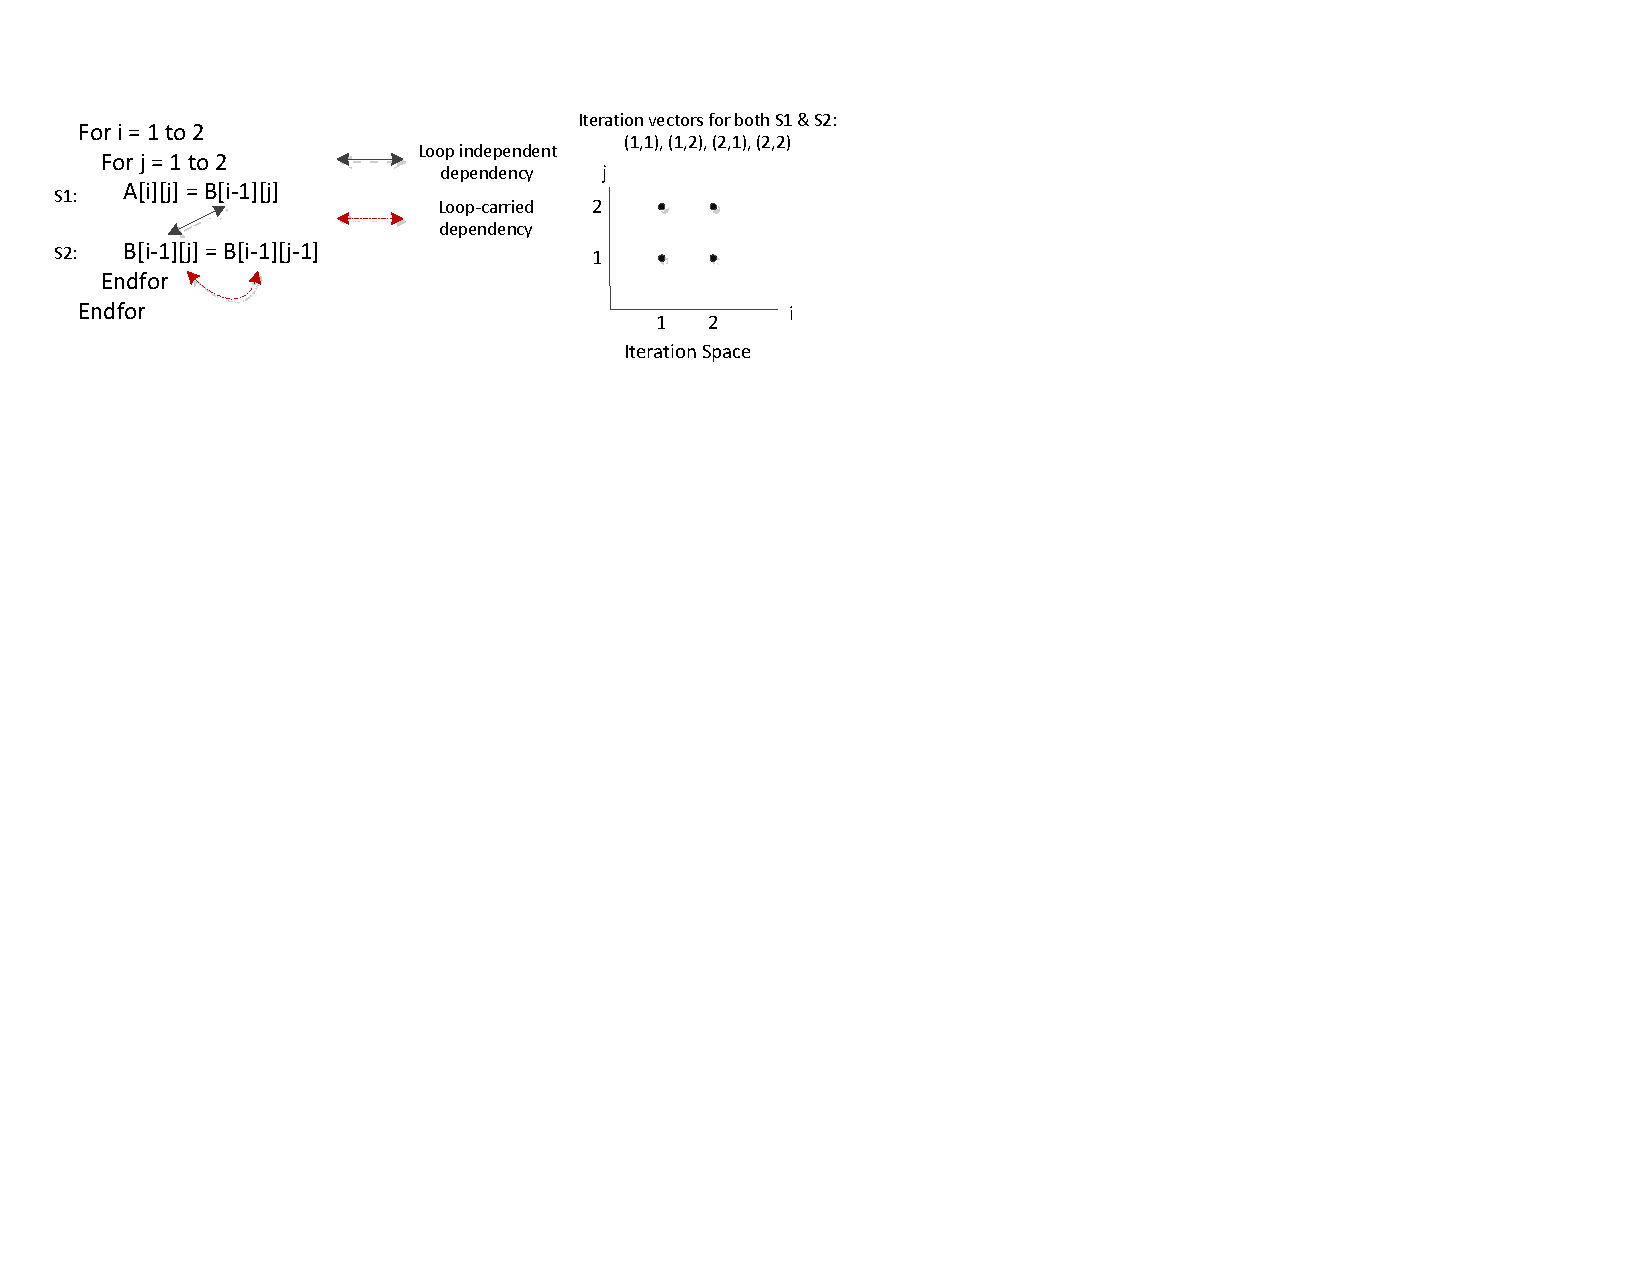
\includegraphics[width=0.9\linewidth]{chap6fig/iterationSp.pdf}
\caption{Dependencies in a Loop Nest
\label{fig:inivis}}
\end{center}
\end{figure}

To exploit coarse grained parallelism in the loop nest, we need to ensure the
absence of loop carried dependencies at a particular level in the loop nest. There are also simple transformations(e.g. loop interchange) which can move loop carried
dependencies to other loop levels so only loop-independent dependencies are left. To enable the discovery of these opportunities, we need to find, in each statement's iteration space, if they intersect with other statements' accessed memory locations. In general, the memory addresses to be accessed can be arbitrary functions of loop indices and runtime data, which makes it impossible to statically determine if
dependencies exist. There are, however, a  set of problems where
the memory referenced can be analyzed during compile time as the addresses are affine functions of the loop index variables. For loop nests of this kind,
dependency analysis is essentially finding integer solutions for the problem:

\begin{equation}
\begin{aligned}
\label{dioeq}
& \text{} & & f(\vec{x}) = h(\vec{y}) \\
\end{aligned}
\end{equation}
\begin{equation*}
\begin{aligned}
& \text{ where}  & & f(\vec{x}) = a_0 + a_1x_1+...+a_nx_n \\
& & & h(\vec{y}) = b_0 + b_1y_1+...+b_ny_n \\
& & & \vec{x}_{lb} \le \vec{x} \le \vec{x}_{ub} \\
& & & \vec{y}_{lb} \le \vec{y} \le \vec{y}_{ub}
\end{aligned}
\end{equation*}
Or equivalently this linear Diophantine equation:
\begin{equation}
\begin{aligned}
\label{adioeq}
a_1x_1-b_1y_1+...+a_nx_n-b_ny_n = b_0 - a_0
\end{aligned}
\end{equation}
\begin{equation*}
\begin{aligned}
& \text{ where}  & & x_{lb_k} \le x_k \le x_{ub_k} \\
& & & y_{lb_k} \le y_k \le y_{ub_k} \\
\end{aligned}
\end{equation*}

Both function $f$ and $h$ takes a iteration vector from within the iteration space of the statement, bounded by $\vec{x}_{lb}/\vec{y}_{lb}$ and $\vec{x}_{ub}/\vec{y}_{ub}$, and map it to a memory location. When
multi-dimensional arrays are used, variables can be separated such that
we have multiple simultaneous equations which are simpler to solve.
The loop carried dependency in figure~\ref{fig:inivis}, for instance, correspond to the following equations:
\begin{equation*}
\begin{aligned}
-1+x_1 = -1+y_1 \\
x_2 = y_2-1 \\ 
\end{aligned}
\end{equation*}
\begin{equation*}
\begin{aligned}
& \text{ where}  & & 1 \le x_1 \le 2 \\
& & & 1 \le x_2 \le 2 \\
& & & 1 \le y_1 \le 2 \\
& & & 1 \le y_2 \le 2 \\
& & & x_1,x_2,y_1,y_2 \in Z
\end{aligned}
\end{equation*}


This problem is an integer linear program, one of the NP-complete problems.  
There are various techniques~\cite{banerjee}~\cite{gcd}, proposed over the years, to efficiently solve a relaxed version of this problem. 
%can be used to compute if
%dependencies exist between memory references. Essentially they are all trying %to find solutions for the problem:
%Many techniques were proposed for compiling these problems onto variable %processors. 
In our binary-based flow, we also try to target these analyzable loop nests, some of which are especially amenable to FPGA acceleration. 
Identifying these regions from the program binaries, however, poses some challenges. 
%however, is not as
%simple as doing it from the source code.


%This can be done by solving the

%direction vector
%is the way to do it
%To capture the dependencies between statements, \texit{direction vector} are computed between statements.

\subsection{Challenges for Binary-based Analysis}
\label{sec:cfbba}
The regular and analyzable memory access patterns expressed in high
level languages become rather mangled when the program binaries are 
being examined. All memory accesses are pointer based with no high
level information to indicate if the data structures they are targeting
are disjoint. With dimensionality of the arrays eliminated, 
separate variables in original address calculation are now coupled to each other. In essence, we have to perform dependency analysis on a huge linear
array with all all addresses being the result of some run time computation.
Figure~\ref{fig:mangledMem} illustrates how different a
set of memory accesses manifest themselves in the actual high level source code v.s. program binaries.

\begin{figure}[htp]
\begin{center}
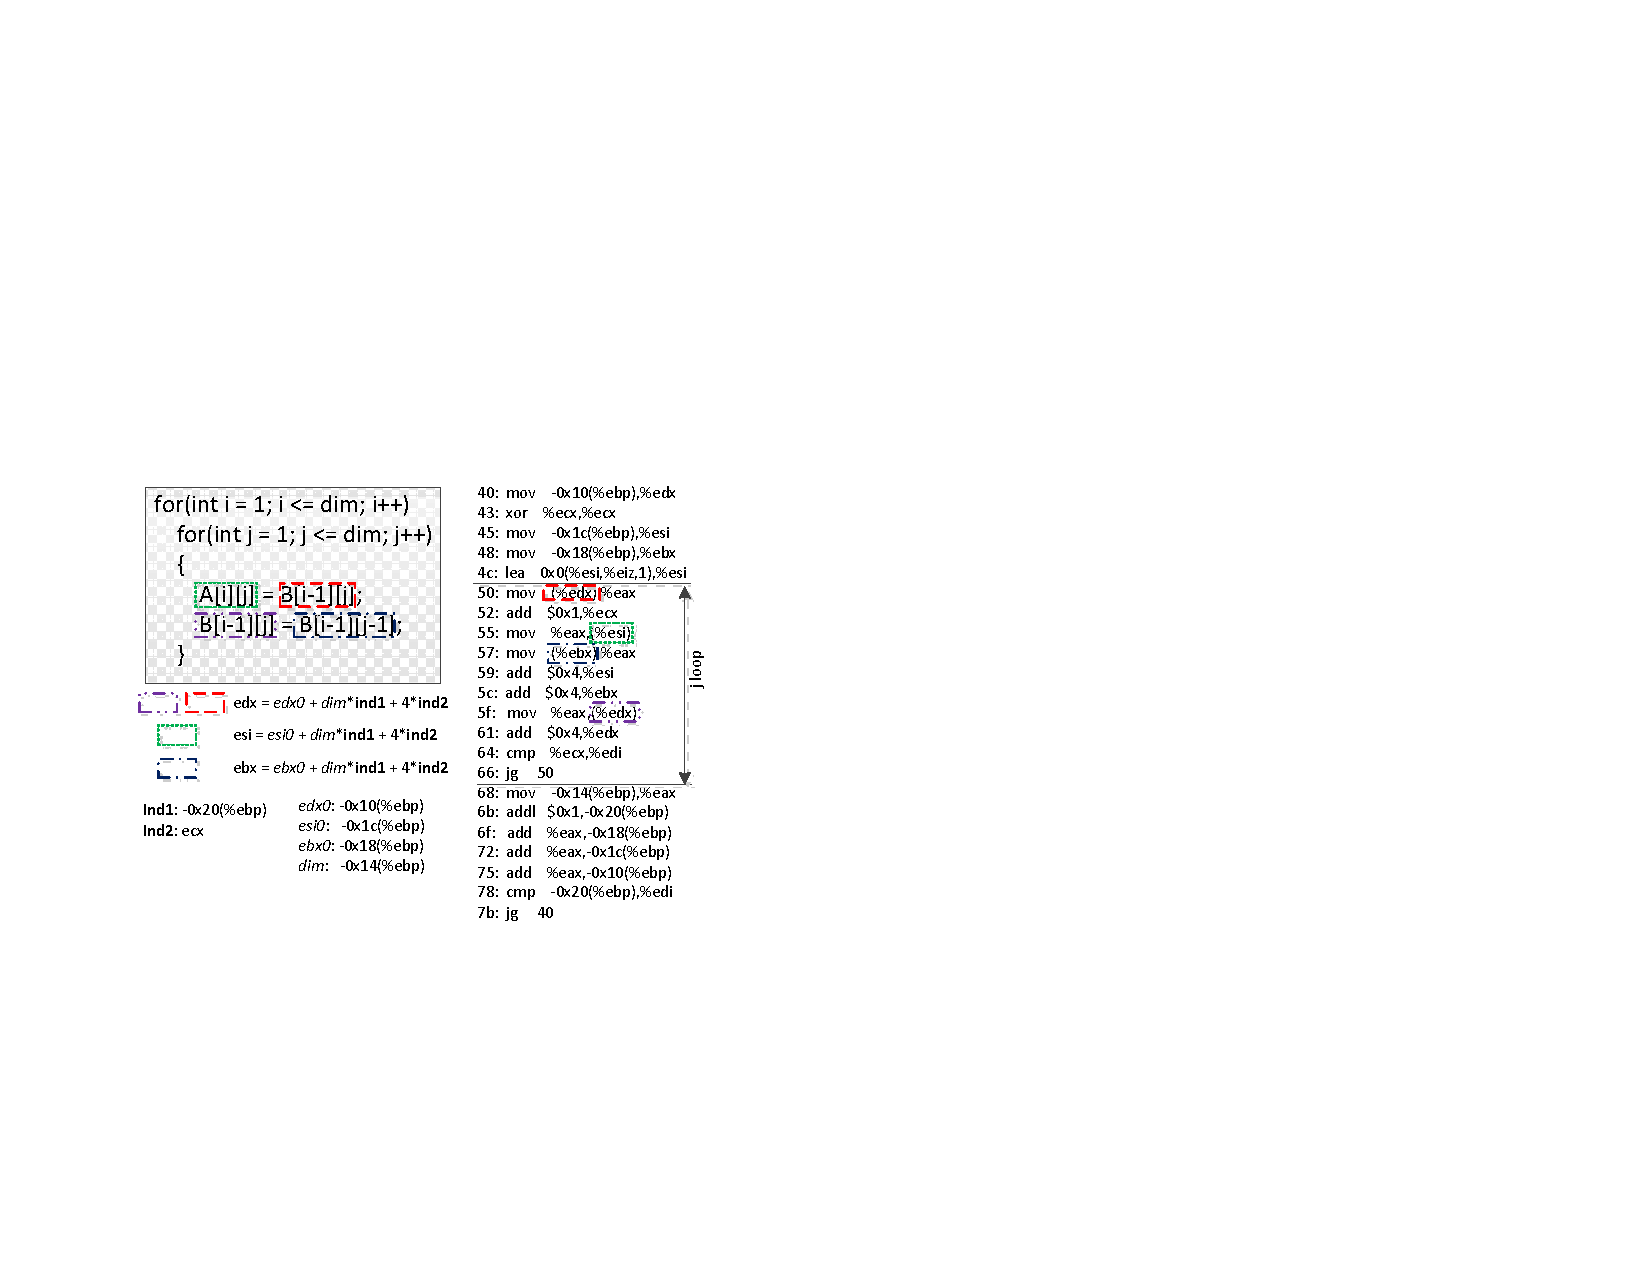
\includegraphics[width=0.8\linewidth]{chap6fig/memBin.pdf}
\caption{Memory Accesses in Program Binaries
\label{fig:mangledMem}}
\end{center}
\end{figure}

In this example, even though the original array references are all affine functions of the loop index variables, in the program binaries, their calculation is much more complex. 
Dependency testing involving only a single loop index in the source code now have to deal with multiple induction variables. More importantly, for equation~\ref{adioeq}, the coefficients ($a_0...a_n$ and $b_0 ... b_n$) are statically known constants while
in the binaries, everything is a runtime data item stored in either a register or a memory location. Naively 
substituting these symbolic variables into the Diophantine's equations yields
a non-linear formulation which can not be solved by the common techniques
in optimizing compilers. On the other hand, %it is relatively straight forward, 
as long as these coefficients are unchanged during the execution of the loop nests, we can leverage various classic dependency testing techniques to formulate a fixed set of checks to be performed during run time. This is possible because the dependency
analysis problem does not scale up with the number of iterations, but rather the number of levels in the loop nest, which is easily recognizable from the static binaries. We therefore can quickly verify our coarse grained parallelization before the invocation of the accelerator, 
avoiding speculative execution and the associated costs. 

In our flow, dataflow analysis is always performed on loop nests to ensure there are no updates to these coefficients during the loops' execution, before more detailed dependency testing and parallelization are attempted. The  potential for actual speed up of course largely depends on the existence of coarse grained parallelism.



%we can be sure that only a fixed amount of computation is needed in
%the dependency. This is not hard to see as the size of the problem formulated 
%does not depend on the actual values of the variable but the number of levels in the loop nest.

%we can assume they are runtime constant and the dependency analysis
%can be carried out. 



%Our approach to deal with this uncertainty is described later in section~\ref{makingAcc}.





\subsection{From Dependency Testing to Parallelization}
\label{sec:fdtp}
%With the dependency testing done, we need to examine the loop nests' potential for parallelization.

To identify the opportunities in parallelizing a loop nest, the dependency distance and direction vectors~\cite{opac-b1000180} are used.
%One way to bridge this gap is through the use of distance and direction vectors~\cite{opac-b1000180}. 

\begin{figure}[htp]
\begin{center}
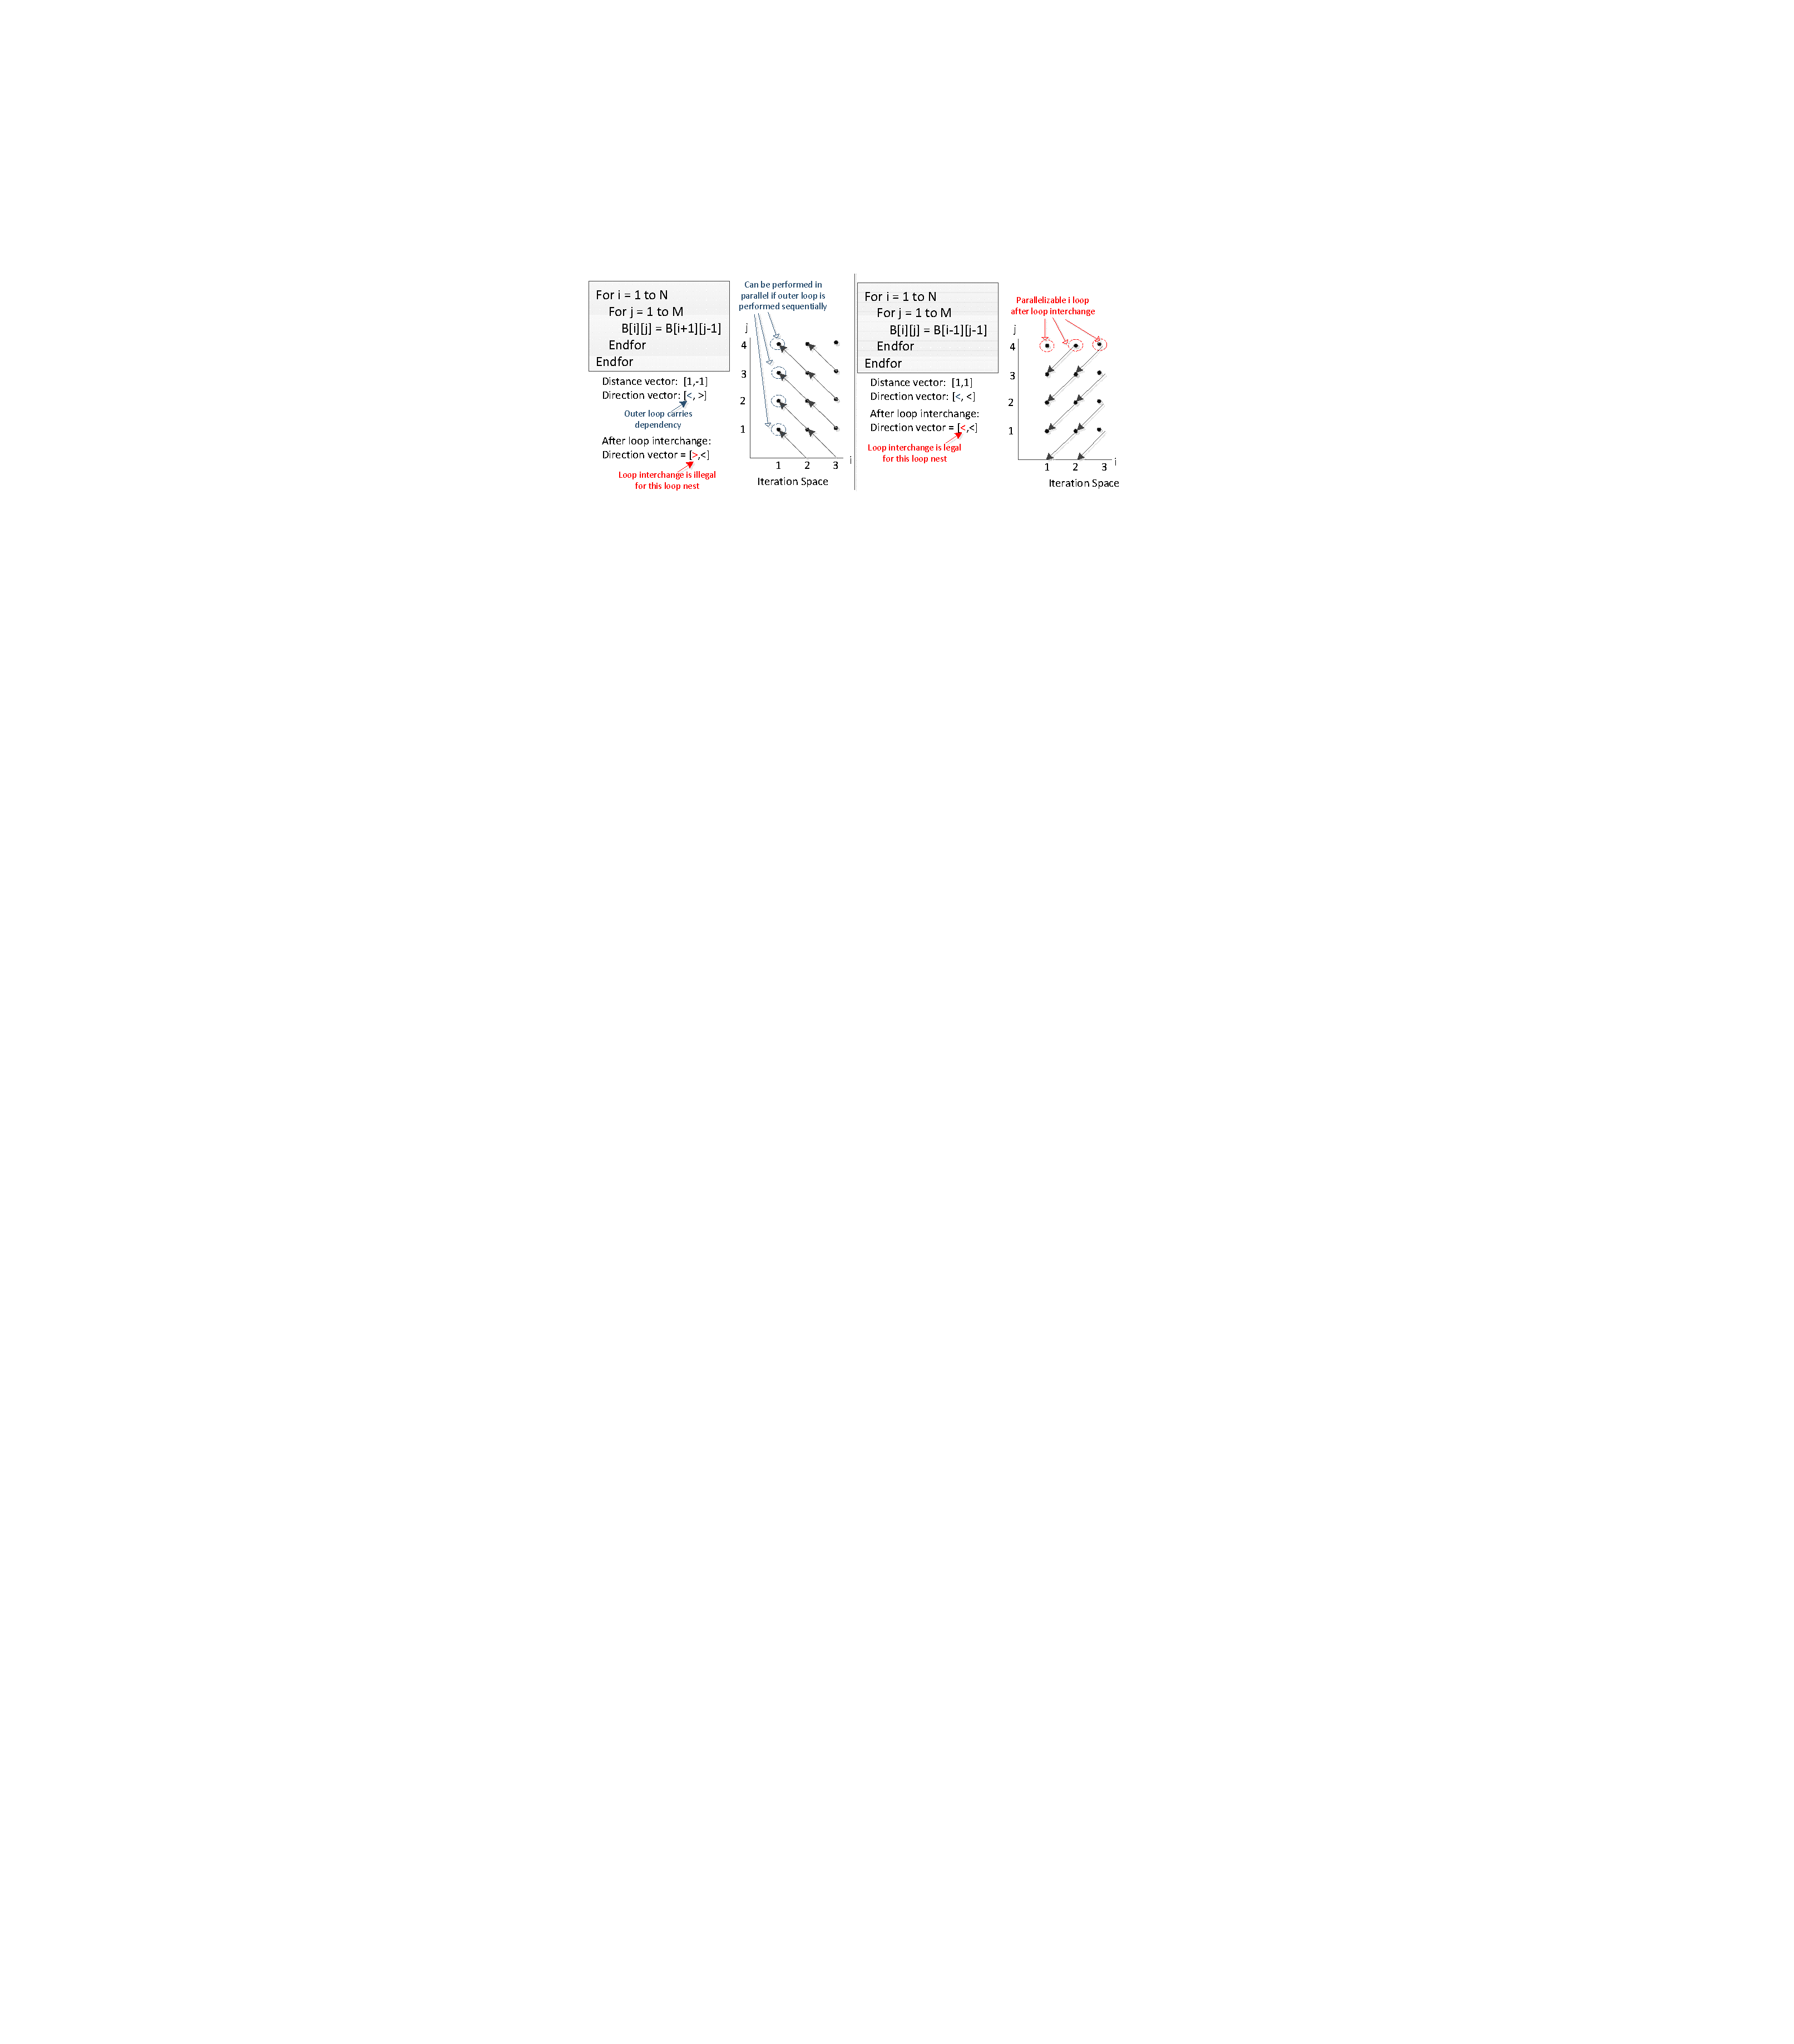
\includegraphics[width=1.0\linewidth]{chap6fig/paral.pdf}
\caption{Parallelization with Direction Vectors
\label{fig:paral}}
\end{center}
\end{figure}
The dependence distance vector can be computed:
\begin{equation*}
\begin{aligned}
&  & & \vec{d}(\vec{x},\vec{y}) = \vec{y}-\vec{x} \\
& \text{ where }&   & \vec{x} \text{ and }\vec{y} \text{ are solution to equation~\ref{dioeq}}  
\end{aligned}
\end{equation*}

The distance vectors give rise to direction vectors $D(\vec{x},\vec{y})$:
\begin{equation*}
\begin{aligned}
  & & ``<" \text{ if } \vec{d}(\vec{x},\vec{y})_k>0 \\
 \vec{D}(\vec{x},\vec{y})_k = &   & ``=" \text{ if } \vec{d}(\vec{x},\vec{y})_k=0\\
 & & ``>" \text{ if } \vec{d}(\vec{x},\vec{y})_k<0
\end{aligned}
\end{equation*}


The convention is to have the lexicographically earlier iteration vector to be
$\vec{x}$ and with that the leftmost non-``=" element of a direction vector would always be ``$<$". 
The index for this leading ``$<$" is also the level of the  loop-carried dependency. 
Assuming a transformation $T$ does not violate loop-independent dependencies,
~\cite{Kennedy:2001:OCM:502981} proved that $T$ is valid as long as
it does not cause some of the direction vectors to have ``$>$" as the leftmost non-``=" component. In addition, any iteration reordering at a level of the loop not carrying dependency is also valid. Using these proven theorems, we can
decide if loop transformations and iteration parallelization are legal when we know all the direction vectors of a loop nest. Figure~\ref{fig:paral} illustrates a
few scenarios where dependency direction vectors are used to determine validity
of transformation/parallelization.








%To summarize, our flow targets loop nests whose direction vectors can be extracted and coarse grained parallelism identified.



\begin{comment}

we leverage several techniques for taking advantage of the discovered parallelism. For the inner most loop, loop pipelining is always applied
to 

Assuming a particular loop level does not carry dependency, 

Comparing against other parallel computers such as multicore or SIMD machines, the 

Parallelization in FPGA vs others:
vectorization ? separate thread? loop pipelining? 


In order to get the dependency vector however, the memory access patterns would
need to be analyzable. Techniques for extracting dependency vectors were outlined in the .... These techniques generally require the array references
to be affine functions of the loop indices, where the coefficients are
all constants. 
Unfortunately, in the case of accelerating binaries, the coefficients are 
always variables stored in either register or a memory location. Naively
substitutes these variable into the Diophantine's equations yield
non linear conditions...As a result, even if the underlying computation are parallelizable, it is a lot harder to verify with the program binaries
as the starting points. It is relatively straight forward, however,
to detect if these coefficient are changed during the execution of the loop nests. 
\end{comment}

% we want something analyzable ---- % but of course even if the source code
% is analyzable, the binary may not be


\begin{comment}
Schemes for checking 
%

This is certainly compatible with the how conventional FPGAs are used
in most applications, where entire compute intensive loops are offloaded
and sped up.

Even as we focus on speeding up loops with large iteration count,
certain loop nests are just difficult to accelerate using FPGAs.
%especially
%when all higher level information is stripped away, as is the case with program binaries.
Due to the slower frequency of FPGA accelerators, it is not sufficient to just exploit instruction level parallelism. For there to be any net gain
in performance, coarse grained parallelism at the loop level has
to be extracted. To establish independence between different loop iterations or perform transformation to extract coarse grain parallelism, the 
\end{comment}


\section{A Two Phased Approach for Accelerating Program Binaries Using FPGA}
\label{makingAcc}
As the accelerator synthesis, which also includes the traditional FPGA CAD flow,
can take hours to finish, the loop transformation/parallelization need to be performed offline. We therefore have to obtain the direction vectors 
before running the actual program. 
In this work, Banerjee's test~\cite{banerjee} is used to find these vectors. The required coefficients for equation~\ref{adioeq} are extracted from past runtime profiles. The dependency testing and parallelization performed during this \textit{offline phase} are  thus a reflection of the programs' past behavior. When the accelerator is actually running, the input data would have changed. The \textit{online phase} thus includes a mechanism to guarantee the 
semantics of the program is not violated by the reordering performed during
the accelerator synthesis. As we have mentioned in section~\ref{sec:cfbba},
a verifying function is invoked before the accelerator, ensuring the correctness
of the overall execution. 



This online phase test is also one of the reasons why we choose Banerjee's method for our dependency testing even though it is not the most accurate dependency testing method
available. The Banerjee's inequality tests for existence of any real solutions for the Diophantine's equations. Since it only tackles the non-integer relaxation of the ILP formulation, the results obtained are conservative.
It will never report lack of dependencies when one exists,  but may report false dependencies, i.e. when all the real solutions are non-integral.
 More accurate tests like~\cite{omega} find integer solutions but are more costly. Since we are
going to perform the test again using runtime data when the accelerator is actually
being invoked, the faster, though more pessimistic, method is preferred.

When applying Banerjee's method, a particular direction vector $\vec{v}$ is subjected to test, and the result reveals if a pair of memory accesses are dependent in $\vec{v}$'s direction. 
%first used as the constraint and the result of the test reports if this vector may hold true for a pair of memory accesses. 
%Therefore, 
To find all the direction vectors for dependencies, a hierarchy
of tests are therefore involved. For a pair of memory accesses in a two level loop nest, the possible tests are shown in figure~\ref{fig:testingHier}, where ``$\ast$" denotes a union of ``$<$", ``=" and ``$>$". Negative test result from any node in the hierarchy eliminates the necessity to continue testing its subnodes. A subset of these dependency direction vectors
are true for each loop nest and dictates what kind of transformations are valid for accelerator synthesis.


\begin{figure}[htp]
\begin{center}
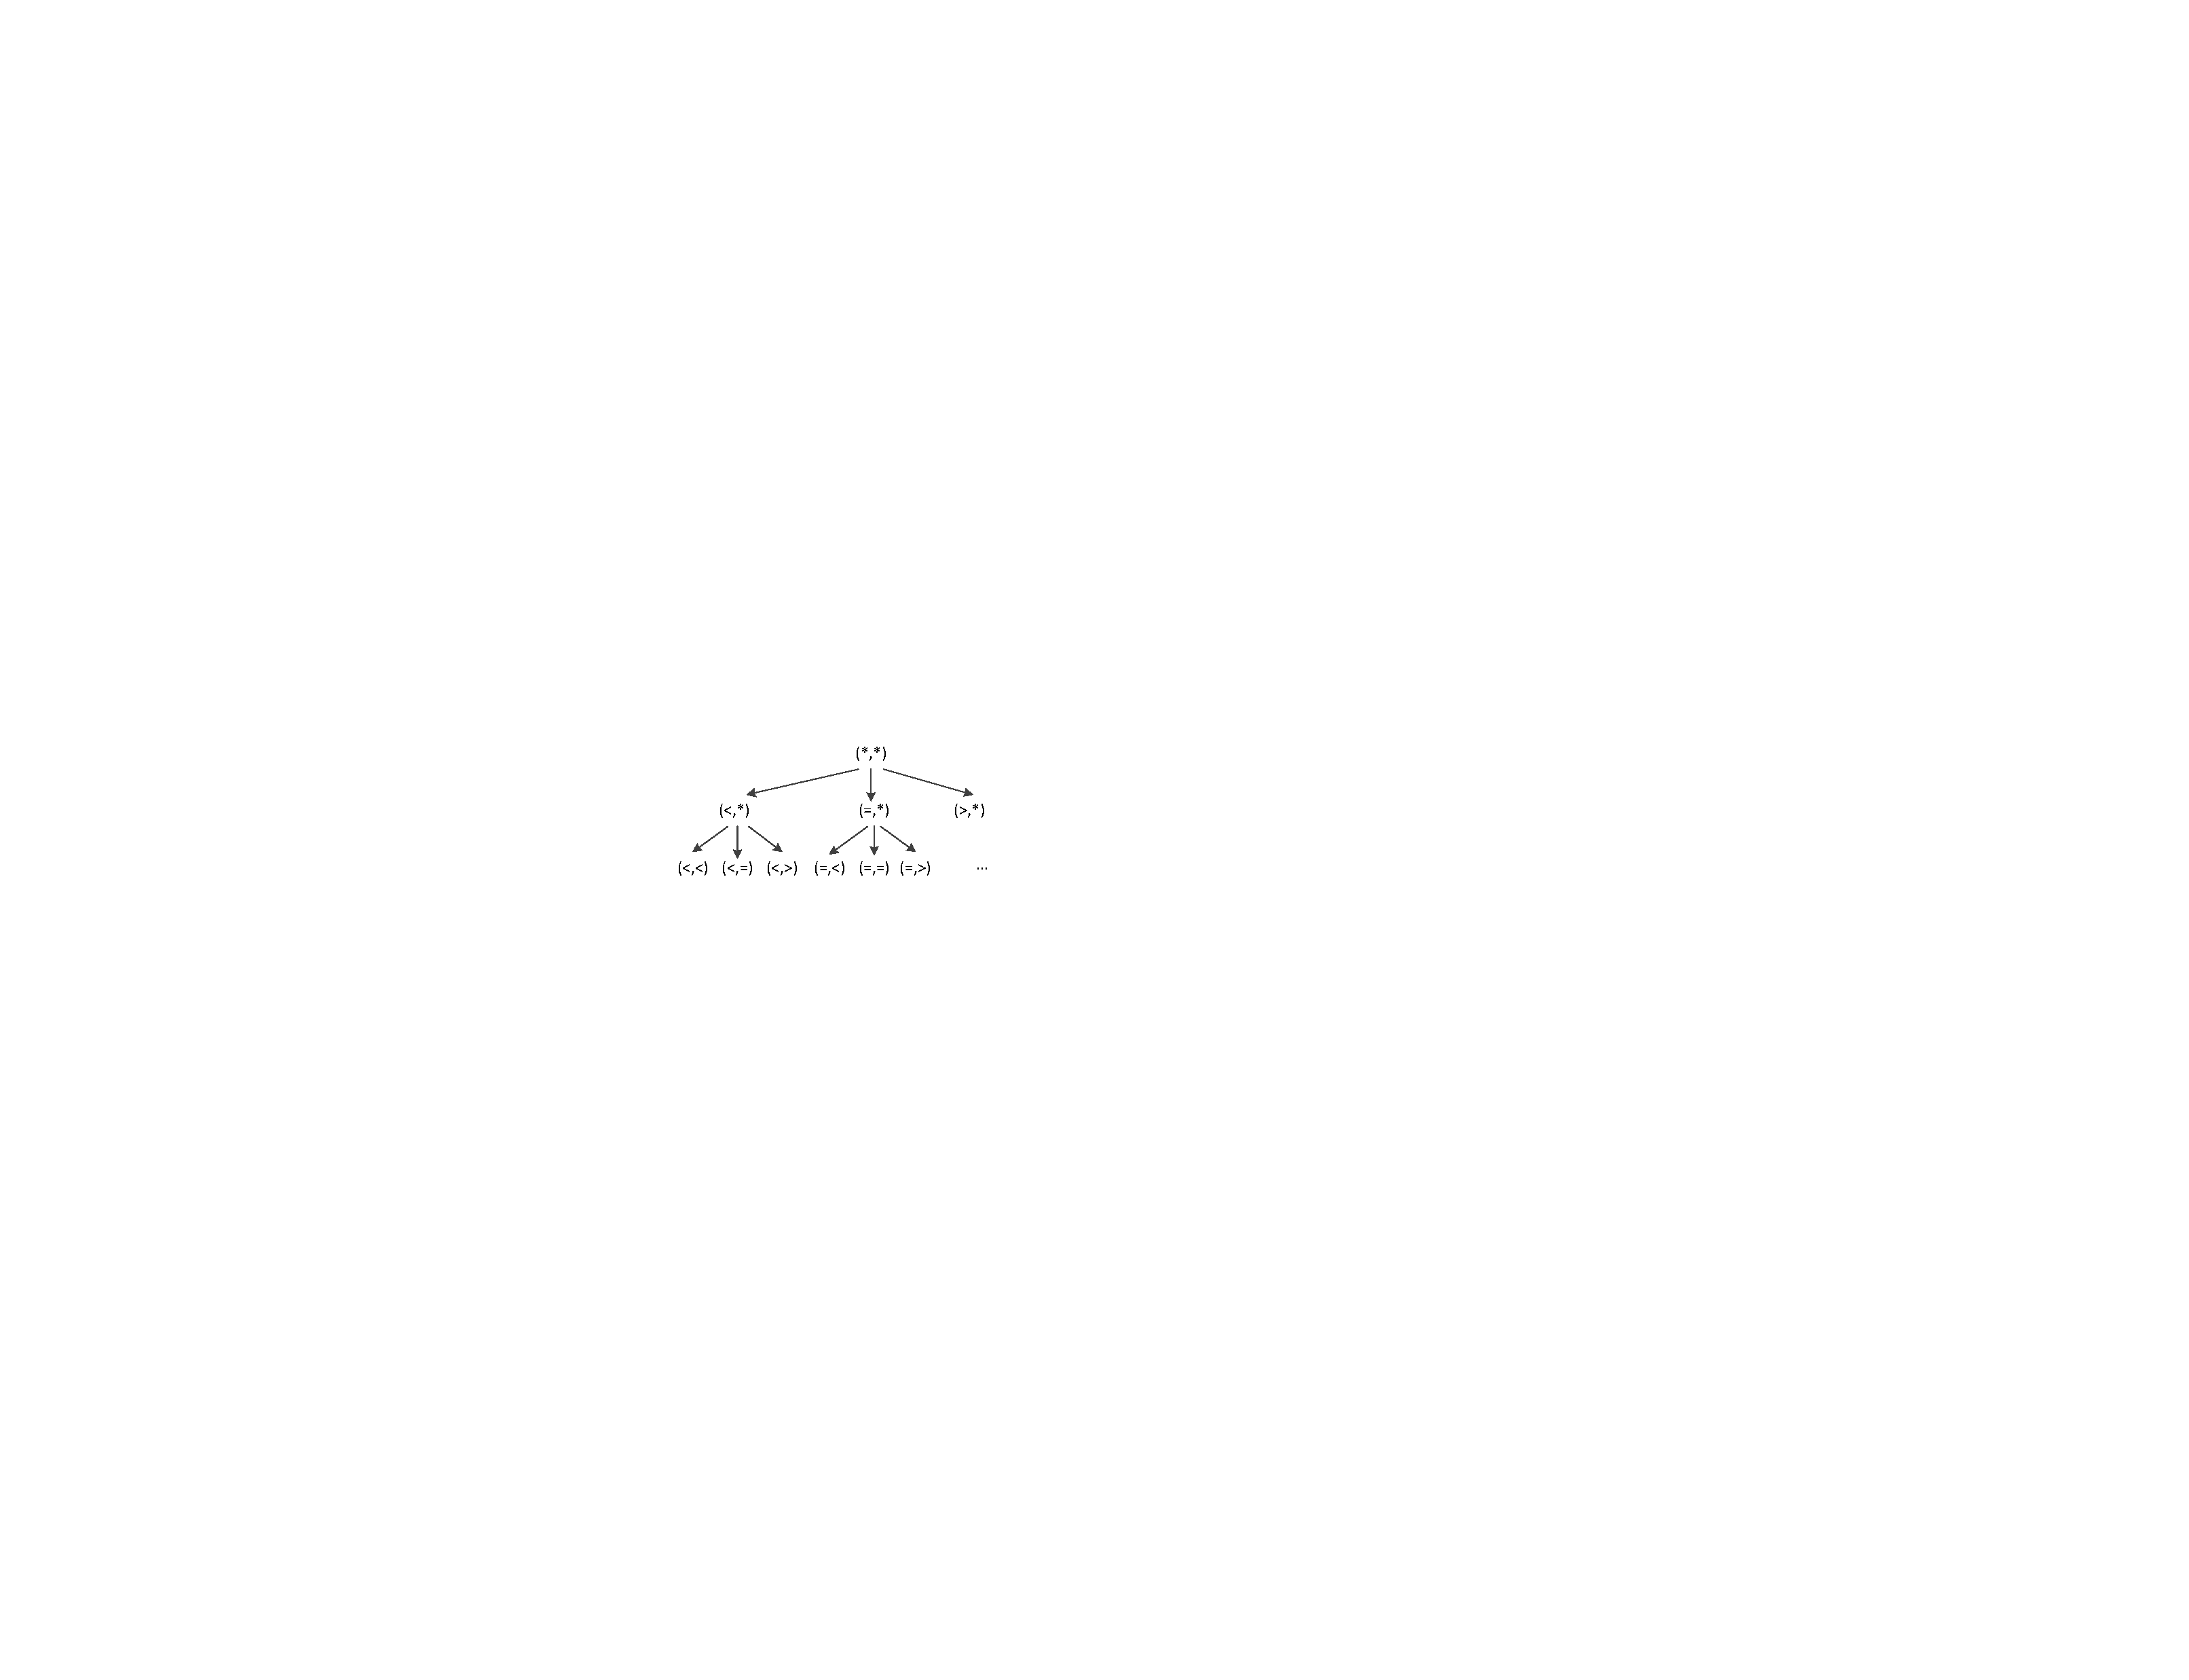
\includegraphics[width=0.6\linewidth]{chap6fig/testingHier.pdf}
\caption{Hierarchy of Dependency Testing for A Two-Level Loop Nest
\label{fig:testingHier}}
\end{center}
\end{figure}



\subsection{Offline Phase: Accelerator Synthesis}

\subsubsection{Dependency Analysis}
To perform the offline dependency testing, we built an analysis pass within the LLVM framework. As LLVM takes C/C++ as input, a preprocessing step is performed
to convert the binary of the selected loops to C functions. It is also in this step when we extract coefficients for the Diophantine equation and bounds for loop indices from past runtime profiles.
The numbers obtained are substituted as constants into the C functions, enabling the subsequent analysis. 
In the original binaries, these variables are often stored in the memory. 
Thus in addition to examining their past values, we also perform a check to ensure their memory locations do not alias with any other references performed by the loop nest, again using the addresses observed from the profile. Most of the time, these locations can be
recognized as part of the call stack, and are normally completely disjoint from
the memory footprint of the actual loop. We can thus easily disambiguate them using a simple
range test. Of course, when the accelerator is actually being invoked, this test would need to be run again, as will be detailed in section~\ref{onlinephase}.


\begin{figure}[htp]
\begin{center}
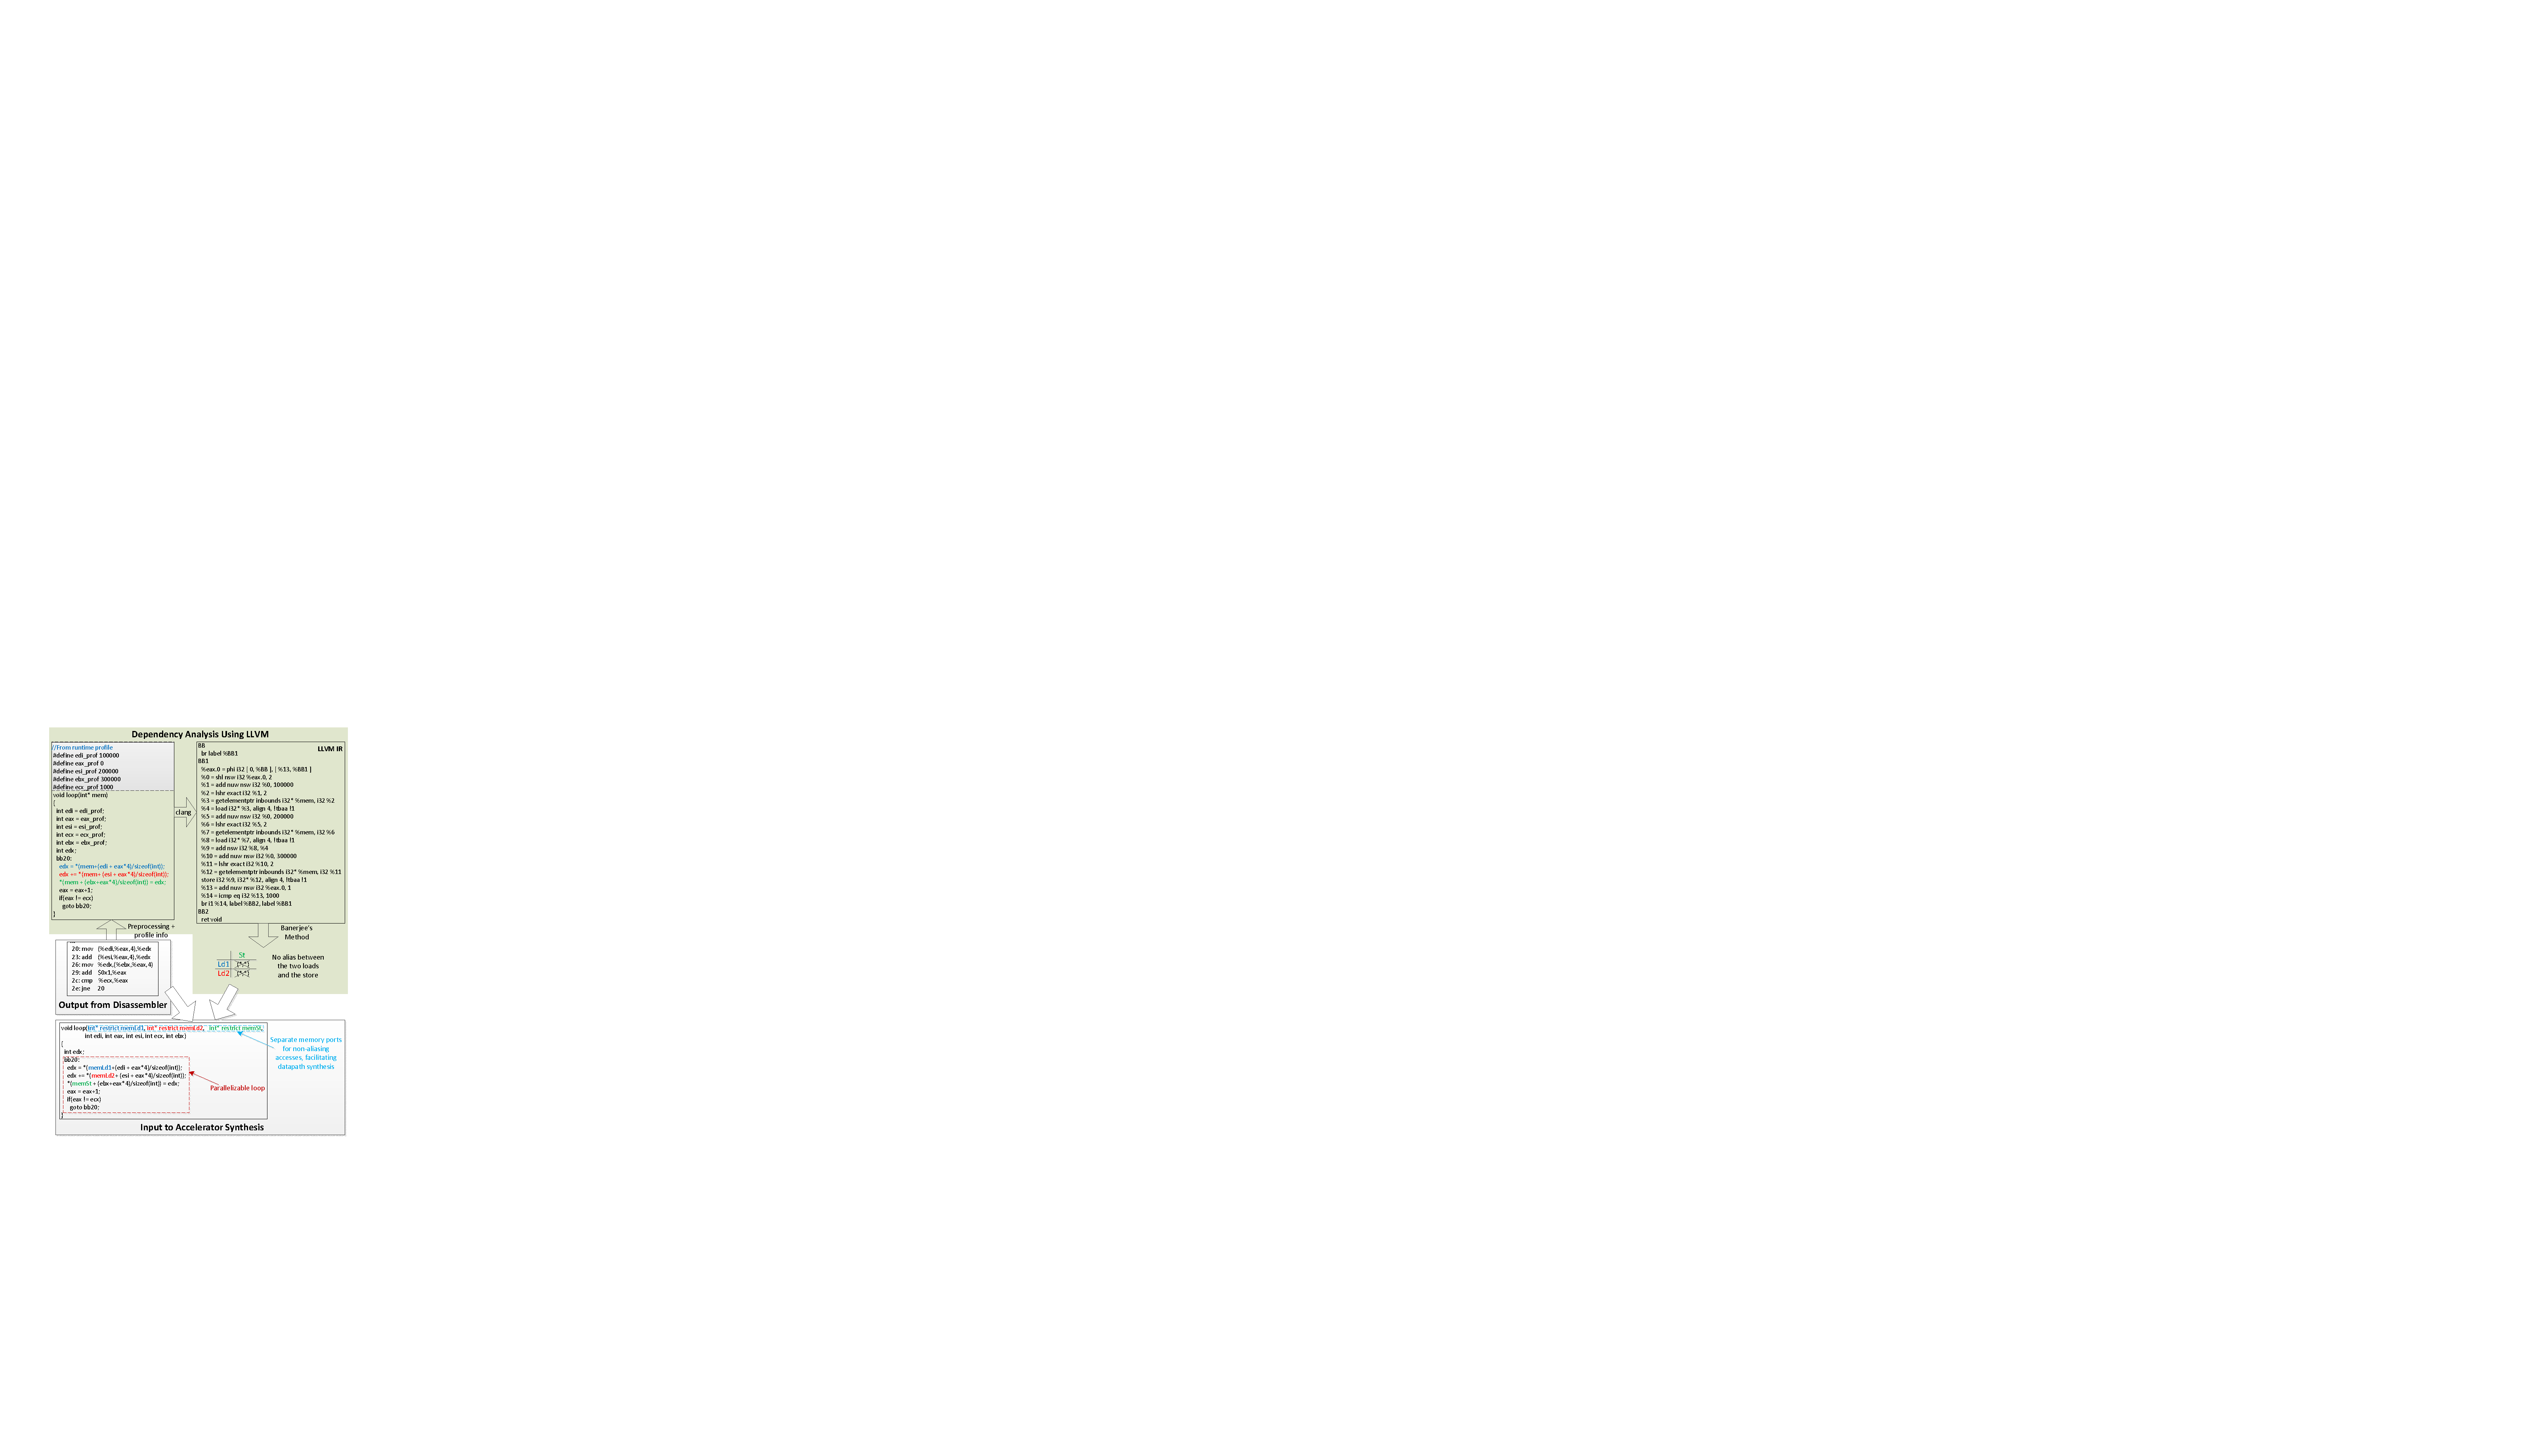
\includegraphics[width=0.9\linewidth]{chap6fig/analysisSteps.pdf}
\caption{From Disassembled Binary to Synthesizable C Code
\label{fig:mainSteps}}
\end{center}
\end{figure}

 
Figure~\ref{fig:mainSteps} illustrates the steps involved in converting binary to a synthesizable C function. 
The original output from the disassembler is used to generate two
different versions of C functions. The first, incorporating values collected from past runtime profile, can be analyzed by Banerjee's method. The results are the dependency directions between memory operations. In this particular case, the store and load operations are found to be non-aliasing. This information is then used to generate the final C function, where each memory access is associated with a different pointer. Whether we
feed this version to conventional HLS or our pipeline generation flow, separate pointer
arguments can be mapped to multiple memory ports, through which data requests can be initiated
independently.

%are applied to a loop doing simple vector addition.%example in figure~\ref{fig:mangledMem}.
\subsubsection{Memory Level Parallelism}
\label{subsec:mlp}
There are actually two levels of parallelization when it comes to scheduling memory accesses during HLS. As shown in the example above, the absence of dependencies between memory operations allows for their association with
different pointers. The scheduling engine in the HLS tool can then schedule
them without being constrained by the original program order. However, multiple pointers may still be assigned to a single physical memory  interface. The structural hazard would then dictate the action of the scheduler,
as a single memory port may only accommodate one load and one store per cycle.
To loosen this structural constraint, it is possible to create multiple memory
ports, each assigned to a subset of pointer arguments. More aggressive scheduling, from the datapath's perspective, can then be performed. In addition, certain memory operation inside a loop can be converted to burst
access when it does not have to share the port with others. This frequently boost the efficiency of the off-chip bandwidth usage.


The precondition for exploitation of any memory level parallelism is of course the non-overlapping of addresses accessed by memory operations. This is especially true if they are to be issued through multiple ports, 
%they need to be completely independent from each other 
as we assume the RTL generation backend, the interconnect and memory subsystem may all be aggressively reordering these requests -- by inferring burst accesses or buffering. Therefore, for every pair of accesses whose ordering matters (i.e. excluding load-load pair), we check the direction vector (*,*,...), and associate each access to a separate
pointer if the test result is negative. In section~\ref{subsec:pmd}, we described how memory barriers are inserted to prevent overly conservative dependency annotation.
Similarly, in our binary based flow, if memory dependencies are carried by outer loops,
memory barriers can also be inserted to facilitate the partitioning of memory access interfaces. The direction vector to test here is  (=,=,..,*,*),
where "=" occupies all levels including and outside of the level of insertion. In essence, we are ensuring any reordering of memory operations within the loop level where the memory barrier is inserted will be valid. An example of this is shown in figure~\ref{fig:withOrWithoutBarrier}. 


\begin{figure}[htp]
\begin{center}
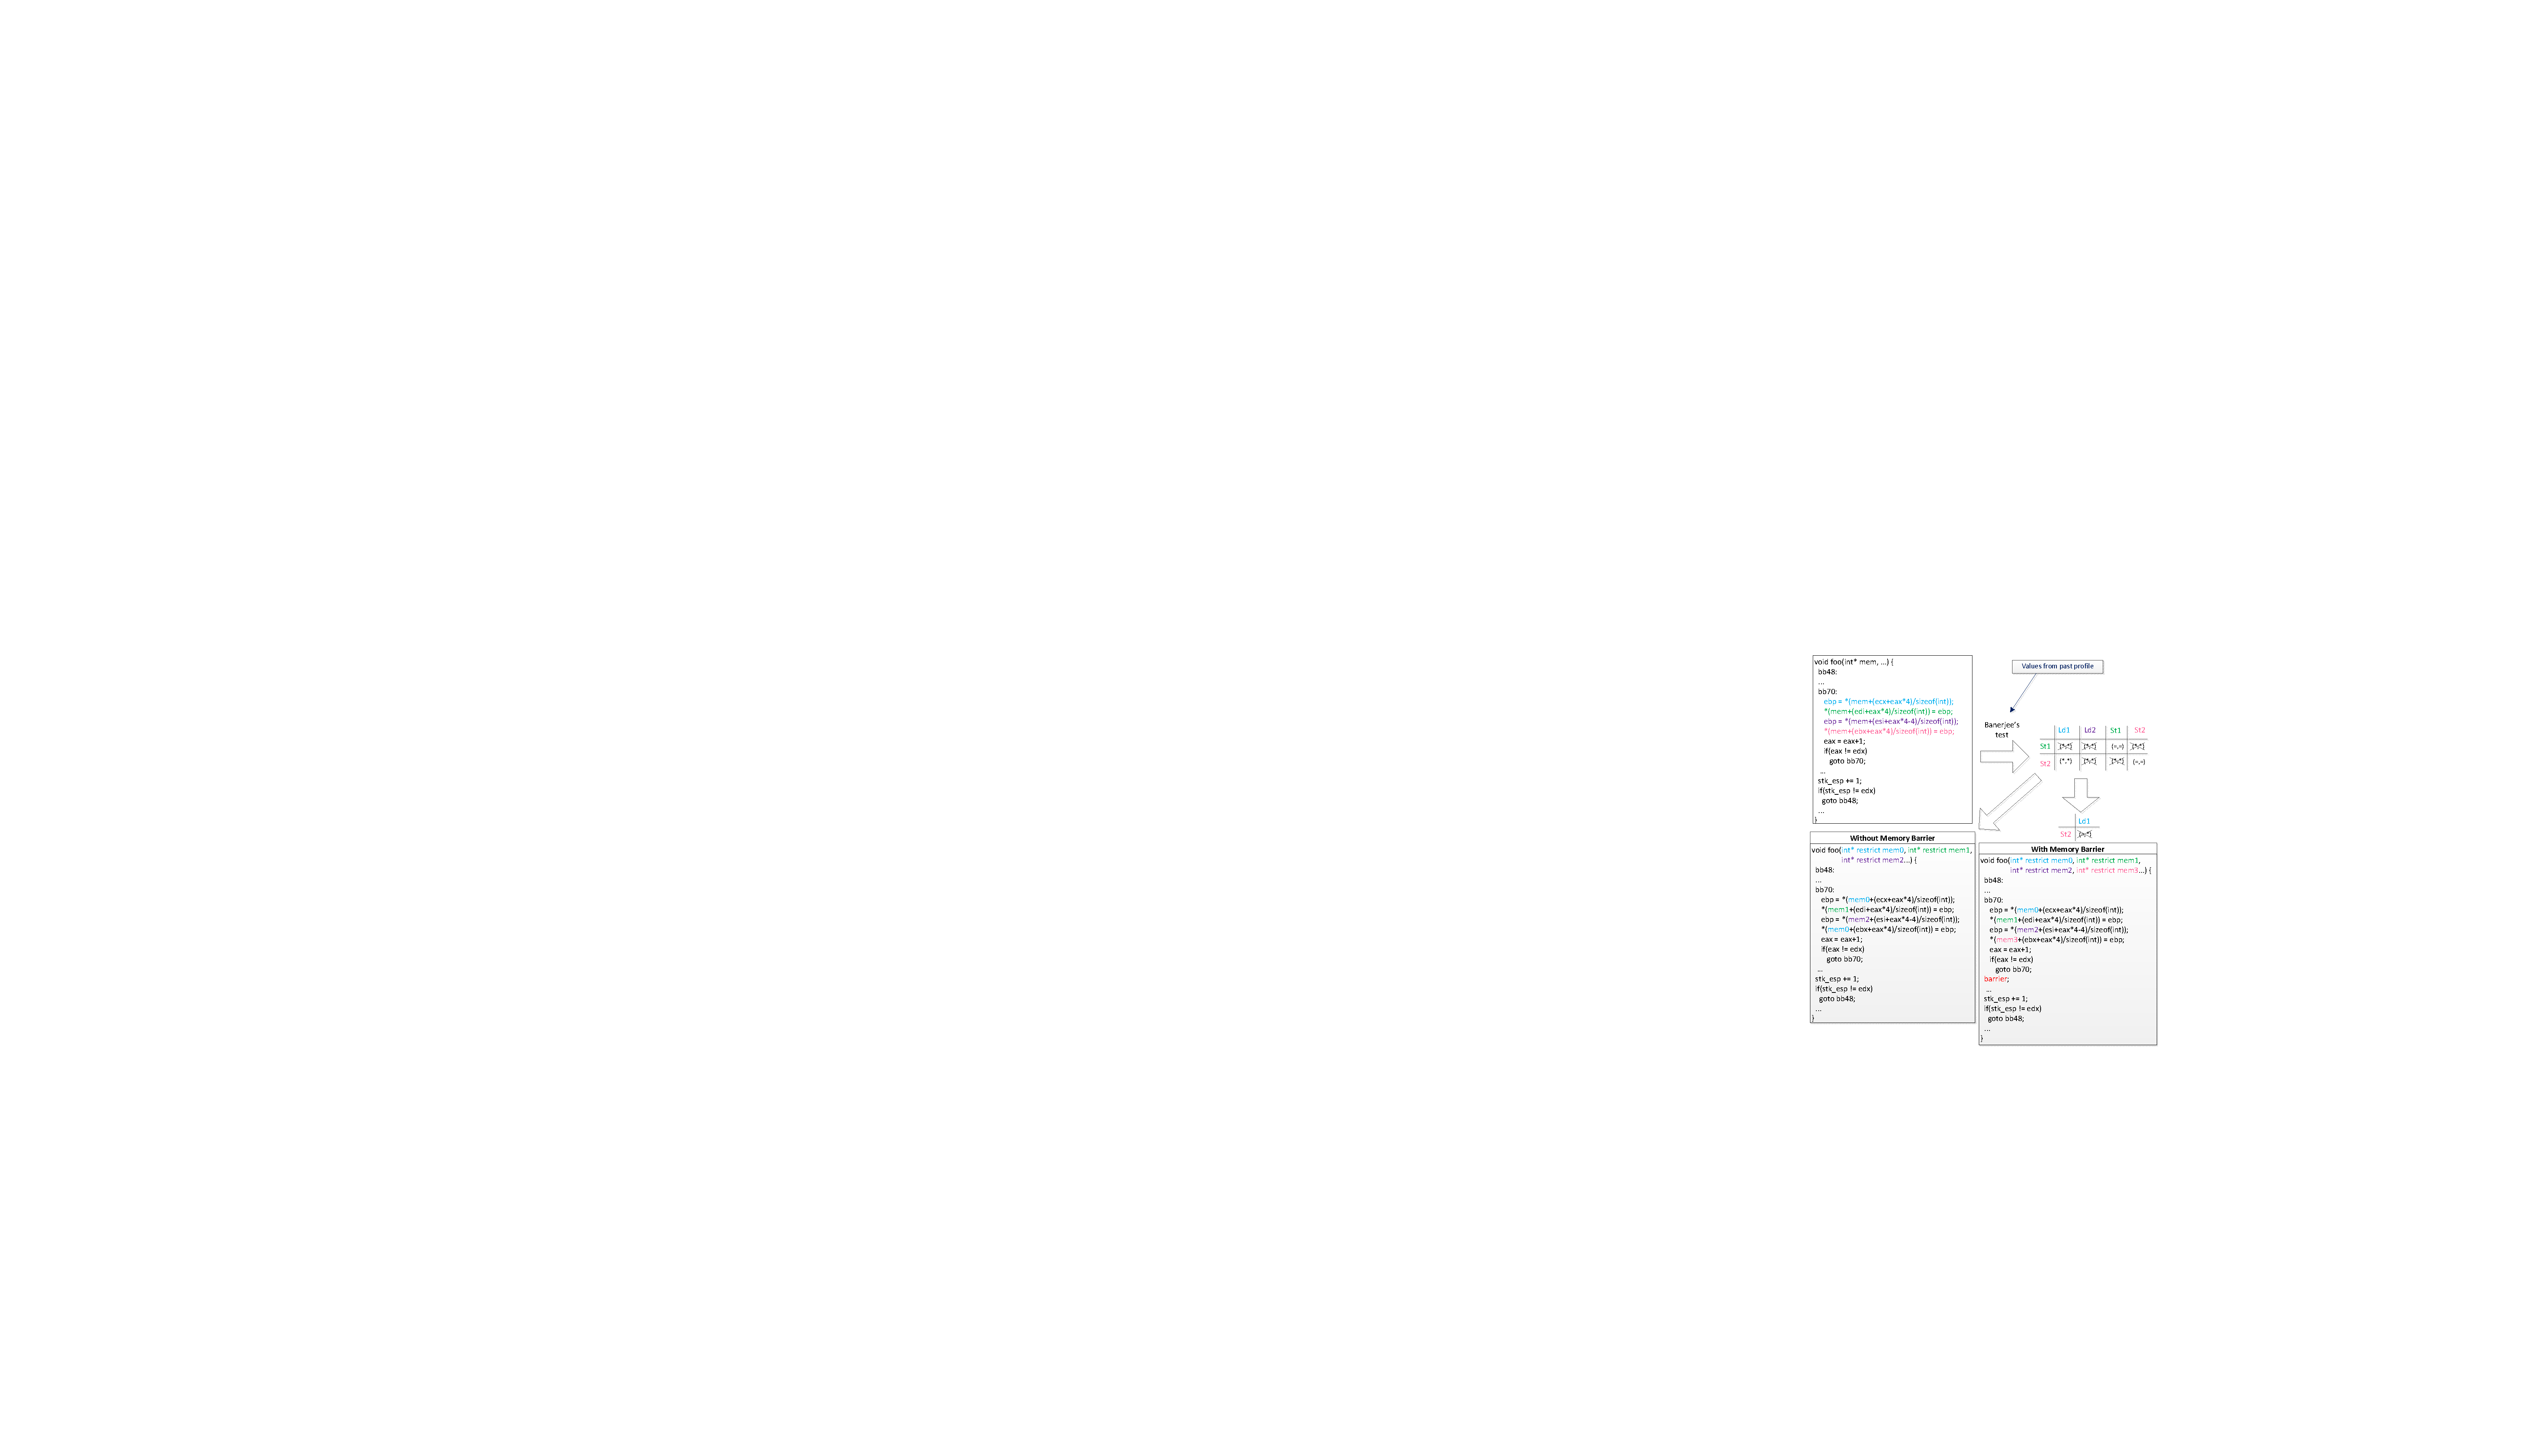
\includegraphics[width=0.9\linewidth]{chap6fig/memOrMemBarrier.pdf}
\caption{Partitioning of Memory Access Interface with Insertion of Memory Barriers 
\label{fig:withOrWithoutBarrier}}
\end{center}
\end{figure}


\subsubsection{Coarse Grained Parallelism}


In addition to memory level parallelism, the loop shown in the example also has coarse grained parallelism between loop iterations. In general, a typical high level synthesis flow can employ several common mechanisms to parallelize loops, as illustrated in figure~\ref{fig:fpgaparal}. 
For the inner most
loop, it is generally very cost effective to pipeline the loop--starting a new iteration before the previous one finishes. If
the iterations are parallelizable, the initiation interval would be 1.
Assuming there are $M$ iterations, the total execution time of the loop
would roughly be $M$ cycles. To further reduce this number, loop unrolling
can be performed. It combines multiple iterations into one, effectively
turning inter-iteration parallelism into fine grained parallelism. 
The iteration count is reduced by the unroll factor ($U$) while the II does not change. Consequently, the total execution time is reduced to roughly $M/U$ cycles with a approximately $U$ fold increase in area. 

\begin{figure}[htp]
\begin{center}
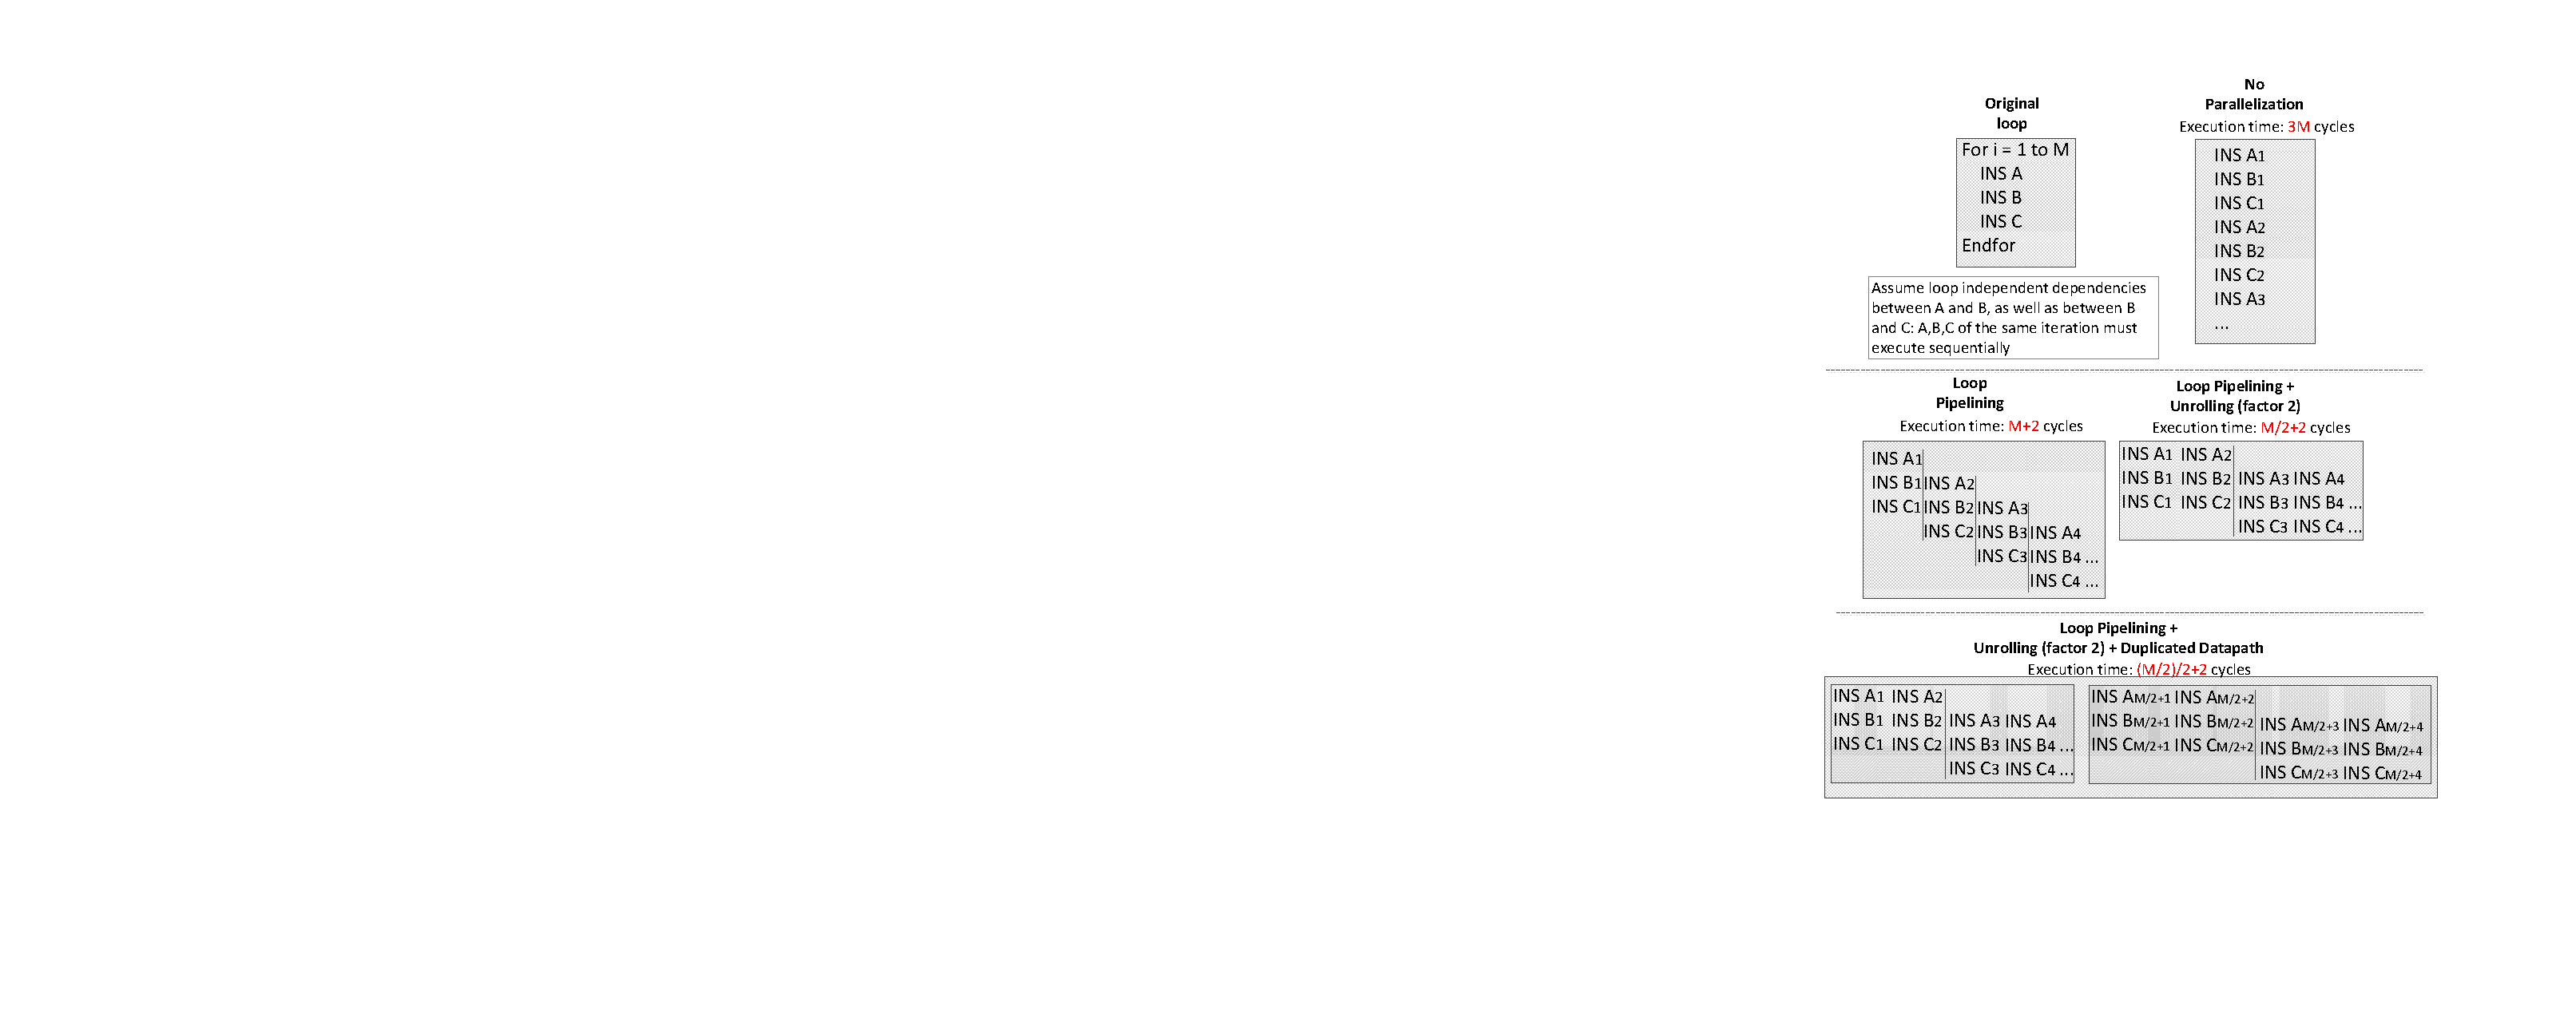
\includegraphics[width=0.8\linewidth]{chap6fig/fpgaParallel.pdf}
\caption{Parallelization in FPGA Accelerators
\label{fig:fpgaparal}}
\end{center}
\end{figure}

To improve the throughput of the accelerator even further, multiple
independent datapaths can be instantiated, each performing a subset of 
the iterations. This technique can be used to parallelize outer loops
as well. For loop with a large number of iterations, this technique provides a good way to trade off more on-chip resources for better performance, although
it also incurs some extra synchronization overheads. Another advantage of
having multiple datapaths is the independence between their controllers.
In an earlier chapter(section~\ref{motex}), we illustrated the vulnerability
of a single monolithic schedule to data access latencies and the resulted
underutilization of the memory bandwidth. In the presence of coarse grained parallelism, it is much easier to fully exploit the data bandwidth provided
by the platform, as each datapath independently generates requests, whether
its peers are stalled or not. 
Certain platforms also provide multiple channels
for off-chip memory access, which can be more easily utilized with duplicated datapaths. 


%Figure~\ref{fig:fpgaparal} illustrates the described parallelization schemes for FPGA accelerators.
\begin{figure}[htp]
\begin{center}
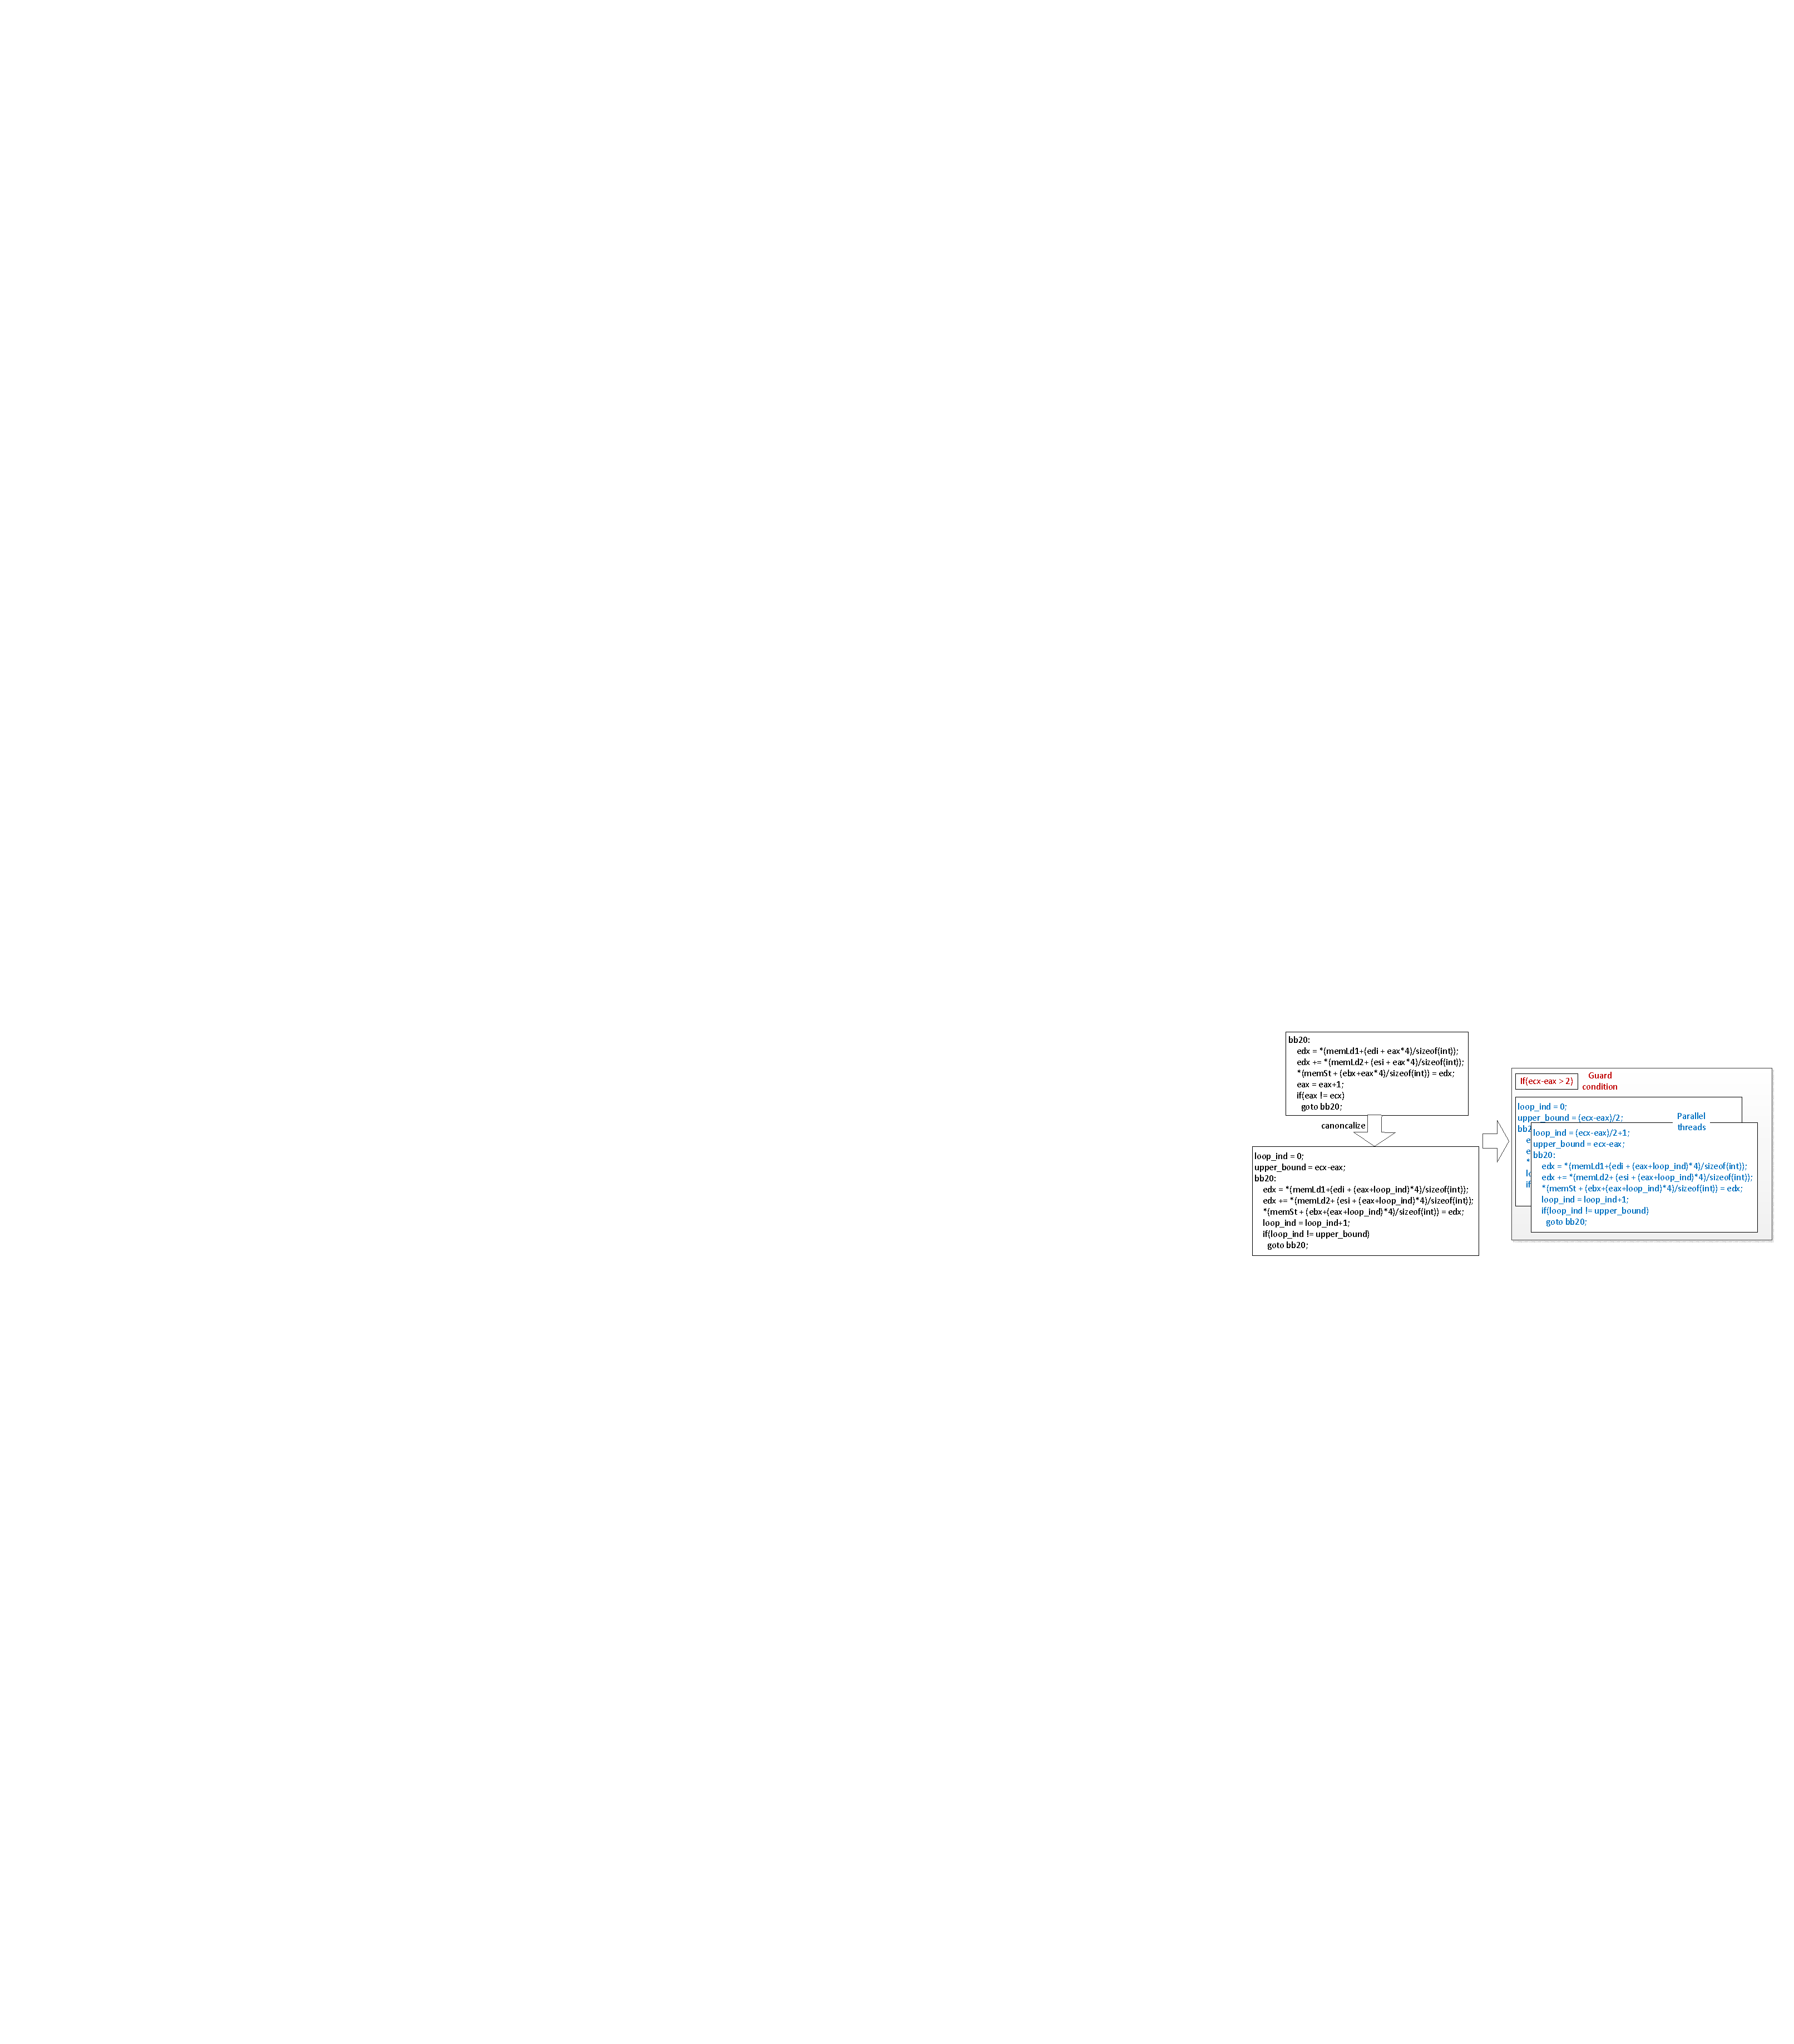
\includegraphics[width=1.1\linewidth]{chap6fig/threadSplit.pdf}
\caption{Thread-level Parallelization 
\label{fig:threadP}}
\end{center}
\end{figure}

We can draw similarities between these techniques and the compiler optimizations targeting architectural features
of various parallel processors. Loop pipelining was a scheduling technique
widely used for VLIW machines, where it is often called software pipelining. Loop unrolling, in the synthesis of FPGA
accelerators, is similar to vectorization, as a wider processing engine
is now used to process multiple iterations simultaneously. The replication of
datapath is essentially generating multithreaded implementation from a serial
specification. Previous research in automatic parallelization can thus be
leveraged for our flow. In this work, we are not trying to invent new techniques, but to enable past work to be applied to program binaries on FPGA
platform. In fact, techniques like loop unrolling and loop pipelining are already built
into commercial HLS tools, and can be easily applied using directives. For thread level parallelization, LLVM can again be used to create multiple functions from a single loop nest. As illustrated in figure~\ref{fig:threadP}, the parallelizable dimension of the iteration space
is to be split evenly, a guard condition is also generated to ensure the validity 
of the derived bounds for all the threads.



\begin{figure}[htp]
\begin{center}
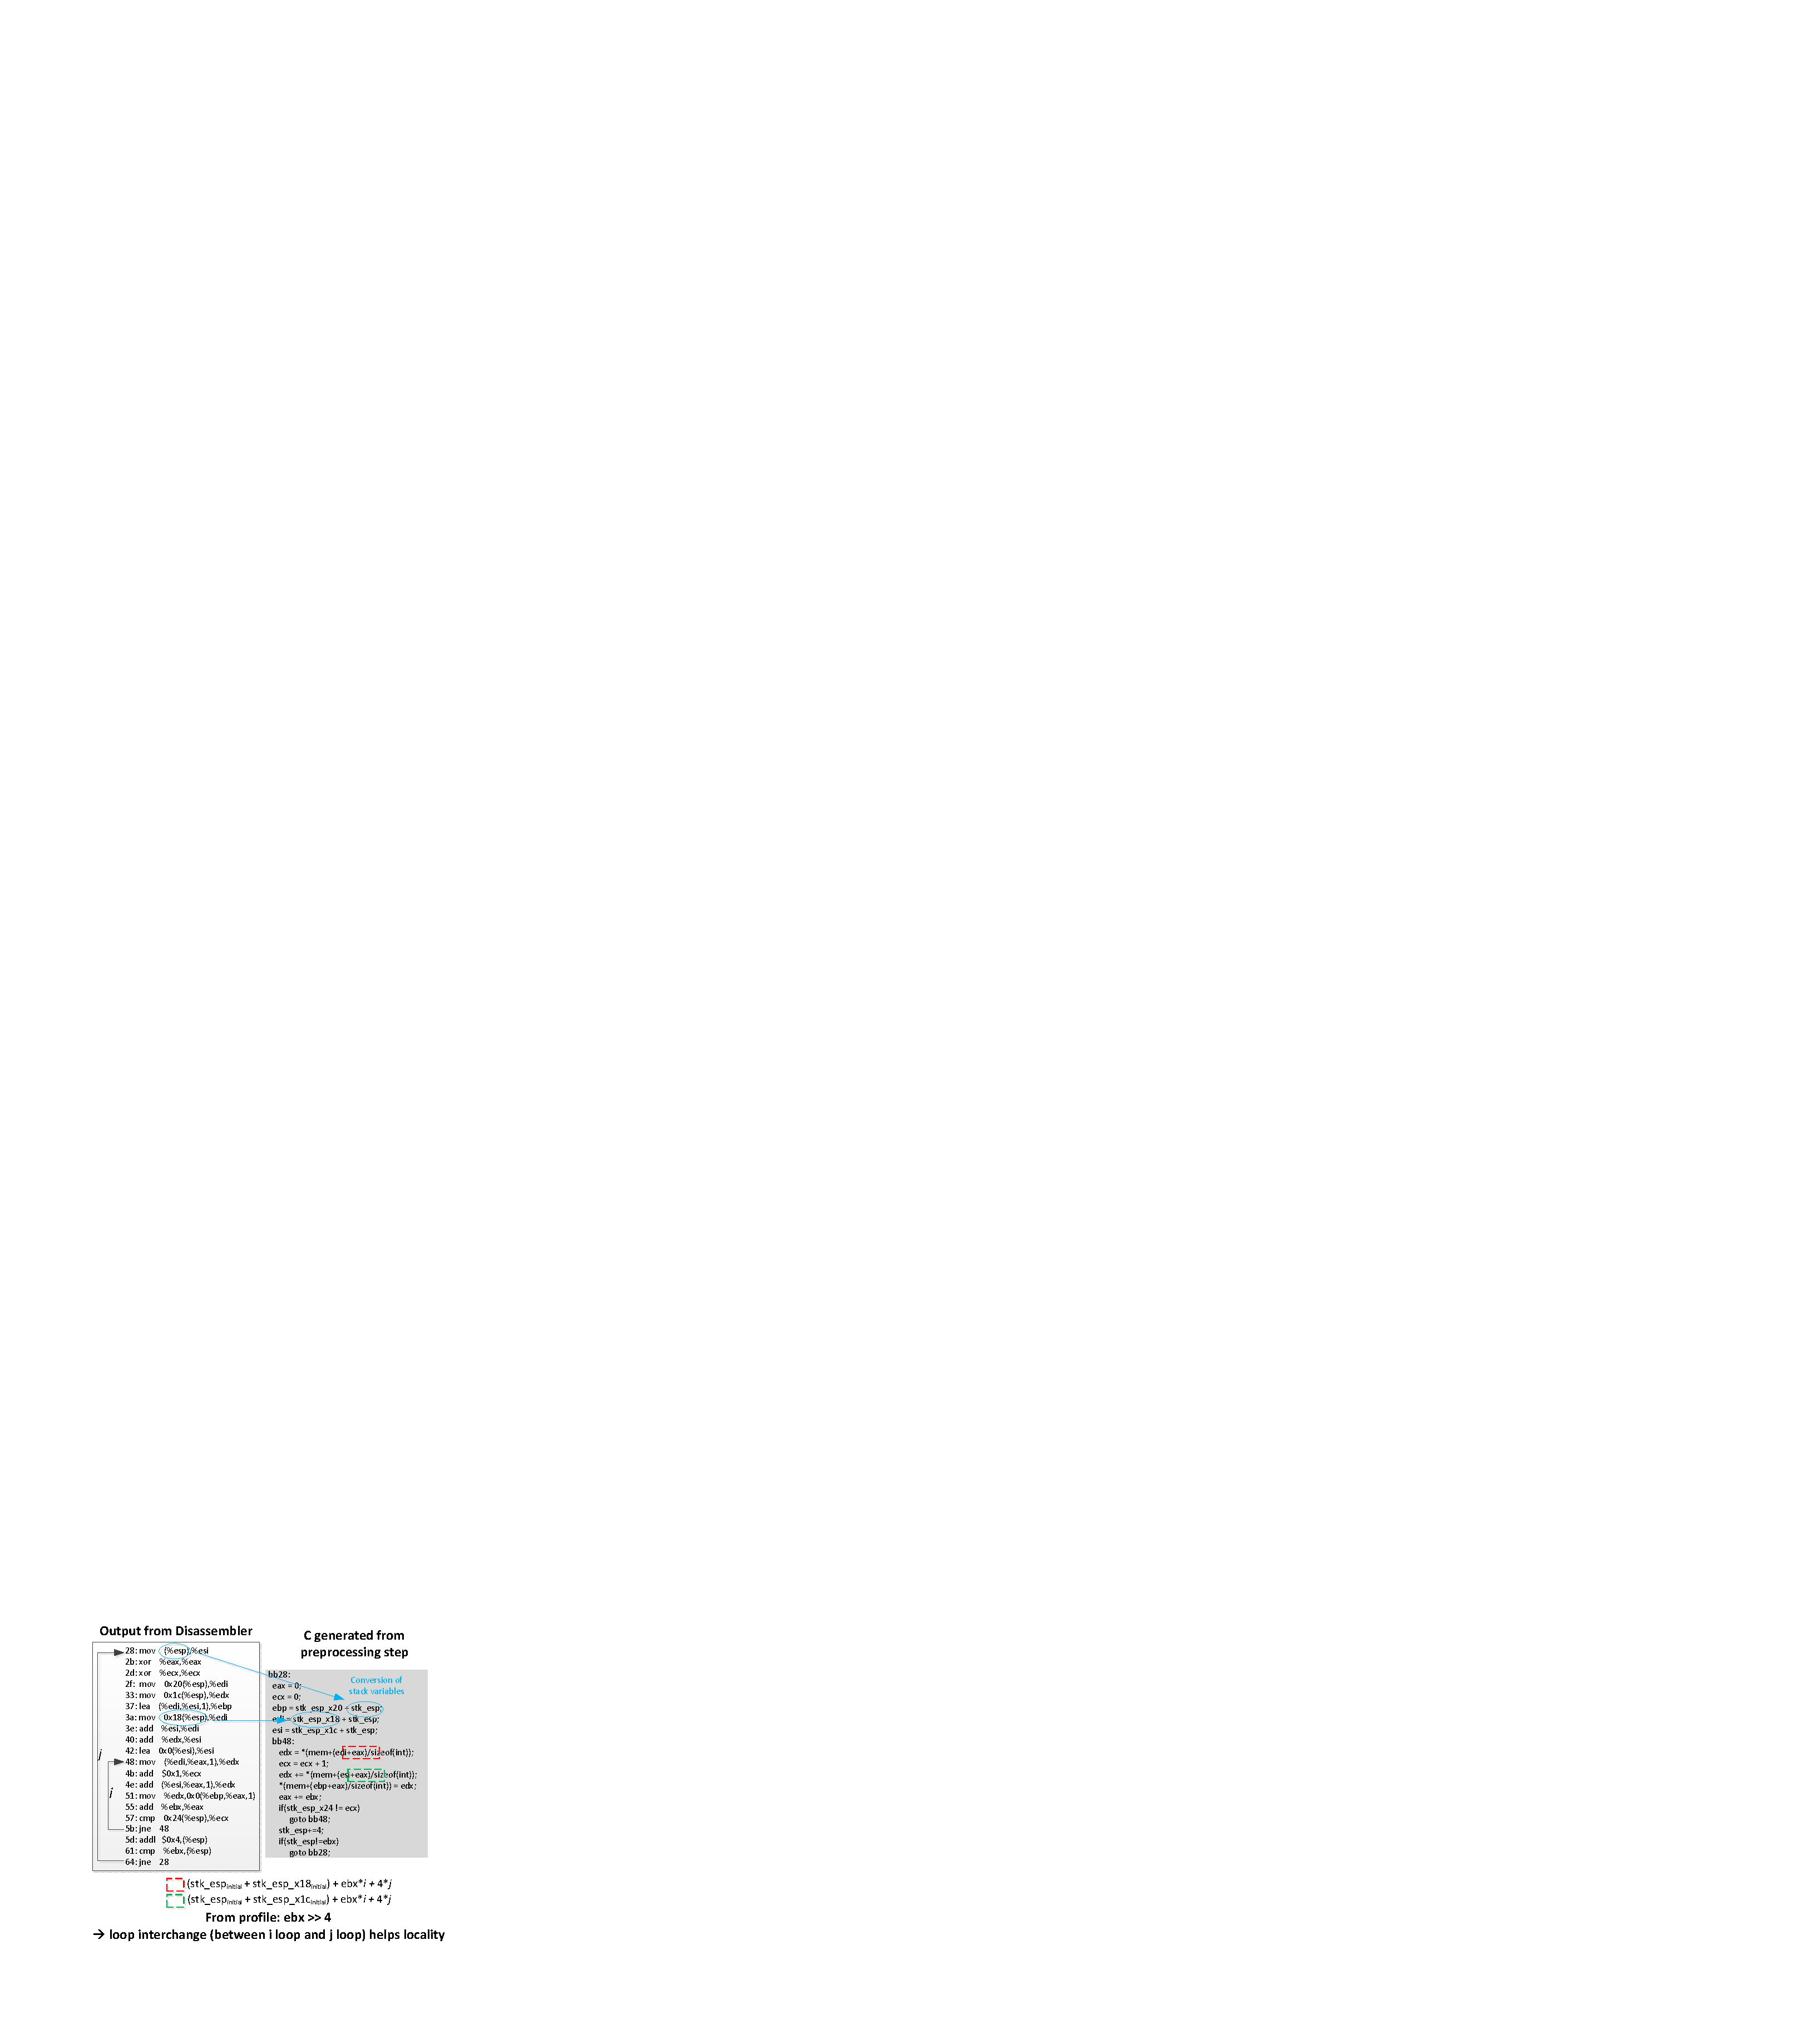
\includegraphics[width=0.75\linewidth]{chap6fig/loopInterchange.pdf}
\caption{Loop Interchange Based on Coefficient Value from Runtime Profile 
\label{localityopt}}
\end{center}
\end{figure}
\begin{comment}
It is particularly interesting to look at the interaction between memory level parallelization and coarse grained parallelization. The pipelining of
loops is a form of instruction reordering, in the absence of memory level
parallelism, the amount of speed up achievable is rather limited~\cite{nwcache}. Similarly, when loops are unrolled, more memory operations are exposed in every iteration of the loop. The increased hardware cost is only justifiable if there are enough simultaneous data streams from the memory subsystem to satisfy the multiplied throughput provided by the wider datapath. The same constraint is applicable to thread-level parallelization as well. For regular computation kernels we target, it is
possible to analytically estimate how much coarse grained parallelization
should be performed given a memory bandwidth budget.
\end{comment}


In our flow, the memory footprint of the computation is assumed to be
much larger than the capacity of on-chip RAM. With the fetching of data
from off-chip storage being a major task of the generated accelerator,
thread-level parallelization is preferred to loop unrolling.
Unrolled inner loop often contain multiple memory accesses which were
initially folded as one operation. In a pipelined inner loop, this
memory access is often converted to burst mode load or store, which is
very efficient. Unrolled inner loop, on the other hand, prevents this burst
inference from occurring as the original single stream of data is now broken
into two interleaved streams.
Loop unrolling makes more sense when the on-chip storage is partitioned into small scratchpad memories which can be accessed by the datapath simultaneously.
Given the regularity of the targeted kernel, it is certainly possible to create a mechanism through which off-chip data gets prefetched and distributed into many distributed on-chip RAM. However, for the benchmarks where off-chip communication 
is the main performance bottleneck, there is little benefit in doing this. 
Also, the overhead of multiple datapath is only marginally higher than unrolled
loop as the main overhead is only the extra control state machine.  



\subsubsection{Optimization for Data Locality}
While FPGAs can exploit parallelism in 
multiple different ways, another important aspect to optimize for would be the temporal and spatial locality of data access. While multiple datapaths can
easily saturate the offchip memory bandwidth, there might be wastage if opportunities for data reuse are missed. 
Even in the absence of data reuse, requests for 
contiguous segments or memory locations close to each other are more efficiently served by the caches and the memory subsystem.
Thus in our flow, we also try to increase the ratio of computation per unit of data communicated with off-chip RAM. By performing loop interchange under the dependency constraints, we can generate multiple versions of a loop nest. To find the implementation with best locality, we would like to have the version with the smaller memory footprint (normalized by iteration count) at the inner loop level.
For our targeted loop nests, the memory addresses accessed are affine expressions of the loop index variables. The coefficient for each of them
decides how large of a stride each iteration takes, which conveniently
approximate how ``unlocal" the memory accesses are. 
Thus for a particular loop index variable, the smaller the coefficient, the deeper its corresponding loop level should go.
This is illustrated in figure~\ref{localityopt}. 



The algorithm used to perform code transformation in our flow is outlined in algorithm~\ref{algoPara}. This is a modified version of the \textit{codegen}
procedure from~\cite{Kennedy:2001:OCM:502981}, which targets vector machines.
Our implementation, in addition to data level parallelism, also try to expose
thread level parallelism at the outer level loop, which can then be exploited by multiple FPGA datapaths. 
The results from our algorithm only provides a starting point for the design space exploration. Even for a single vectorized instruction, combinations of techniques illustrated in figure~\ref{fig:fpgaparal} can be applied to
produce implementations of different performance area trade-off. Meanwhile, 
the supporting infrastructure on the FPGA can also be modified on a per
application basis. The parametrization of on-chip buffer, communication mechanism with external
storage etc. are all parts of the design space. The co-tuning of these ``glue"
structures in conjunction
with the accelerator itself is left to future work.  In section~\ref{biev}, we sample a small subset of the possible design points
to show the trade-off between different metrics.


There are also other transformations which can be applied to extract additional parallelism or to achieve better data reuse. Loop fission and loop tiling, for instance, are techniques used in some optimizing compilers. 
Their incorporation is certainly feasible with our general approach and will
add more dimensions to the design space. 
\begin{comment}

The actual implementation of the parallelization engine is built
on top of the LLVM framework. As LLVM takes C/C++ as input, we created a preprocessing step
to convert the binary of the selected loops to C functions.
It is also in this step when we extract
coefficients for the Diophantine equation and bounds for loop indices from past runtime profiles.
The numbers obtained are substituted as constants into the C functions, enabling the subsequent analysis. 
In the original binaries, these variables are often stored in the memory. 
Thus in addition to examining their past values, we also perform a check to ensure their memory
locations do not alias with any other references performed by the loop nest, again using the
addresses observed from the profile. Most of the time, these locations can be
recognized as part of the call stack, and are normally completely disjoint from
the memory footprint of the actual loop. We can thus easily disambiguate them using a simple
range test. Of course, when the accelerator is actually being invoked, this test would need to be
run again, as will be detailed in section~\ref{onlinephase}.


FIXME:There are many existing compiler passes within LLVM which facilitates the analysis ....
After the transformations, the LLVM IR is converted back to C, before HLS is used
to generate the final circuits. Multiple independent C functions can be generated
when multiple datapaths are desired in the final implementation. Vendor specific
pragmas are also inserted to provide guidance for the HLS tool. An example output,
which targets Vivado HLS backend, is shown in figure~\ref{}. 
\end{comment}

\begin{figure}[htp]
\begin{center}
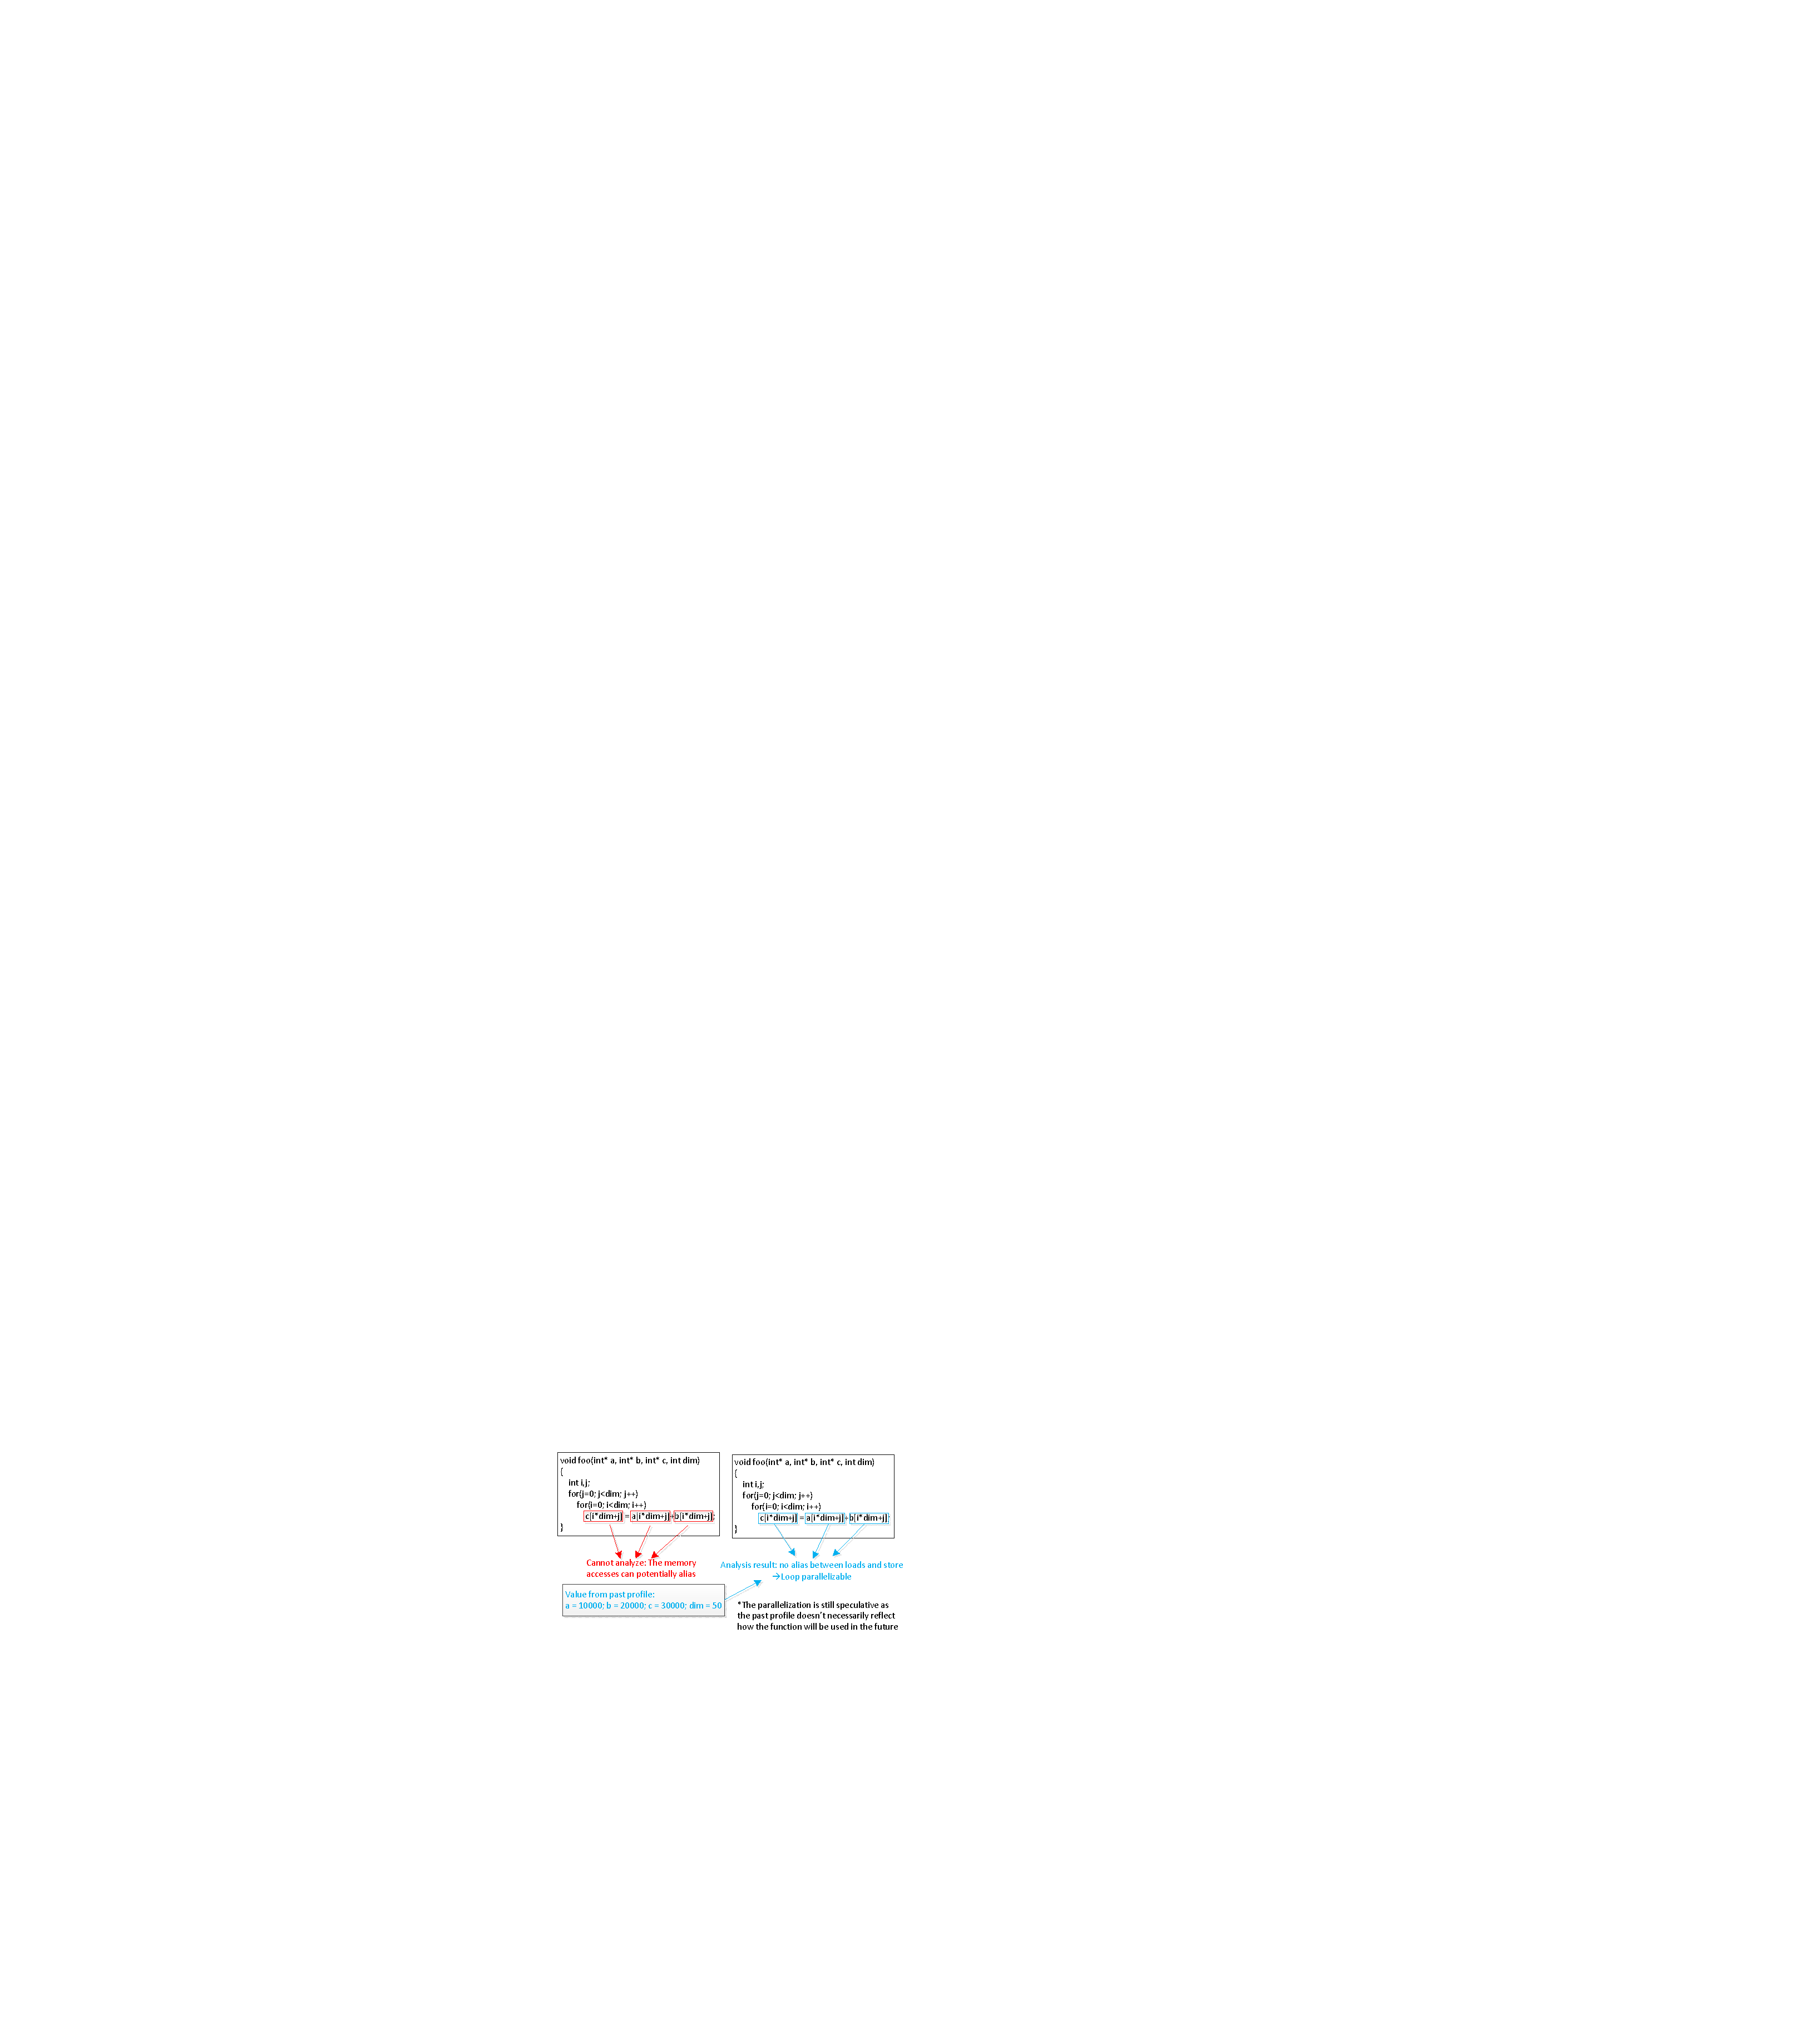
\includegraphics[width=0.85\linewidth]{chap6fig/sourceCodeAnalysis.pdf}
\caption{Analyze Loop in C with Value from Past Profile 
\label{fig:srcAna}}
\end{center}
\end{figure}

It is worth noting that the approach taken in our \textit{offline phase} can actually parallelize certain functions which are not analyzable using only the source code. An example of this is shown in figure~\ref{fig:srcAna}. As the data structures
are passed into the function using pointers, the constant terms (a, b and c) and the coefficient (dim) in the Diophantine equations are all unknown. Banerjee's method, in this case, does not produce affirmative result. On the other hand, with the help of runtime profile,  this function can also be analyzed and produce negative
outcome when tested for the dependency vector (*) -- the loop is parallelizable. 

So far the analysis and parallelization are all performed independent of the actual
RTL generation. In essence we have devised a set of transformations applicable within the LLVM framework. A piece of disassembled binary is converted to synthesizable C code, which is ready to be processed by the hardware synthesis mechanism, be it conventional HLS or the previously described pipeline generation flow. The last part of the \textit{offline phase} involves pushing the RTL through traditional FPGA CAD flow. This step can take between tens of minutes to a few hours,
depending on the size of the design and the utilization of the FPGA chip. 


\begin{comment}
c 2 c
independnet


Even though their location can usually be recognized 
as part of the call stack, we still check for aliasing between 


There are various transformation (e.g. loop interchange passes already
built into LLVM
\end{comment}
%In this work, however, we aim to 

%In addition, as the hardware on FPGAs can be parameterized on a per application basis, there is a huge design space where the high level input
%for HLS as well as the supporting infrastructure (e.g. on chip buffer) can
%be co-tuned. A thorough exploration of this space is left to future work.

%are affine expression of the loop indices, each with a different coefficient,
%The range of memory
%locations accessed by each load/store instructions under each loop level
%is used as a rough approximation of locality. To make the comparison fair, this
%range is also divided by the number of iterations in the corresponding levels.





\subsection{Online Phase: Parallelism Validity Check and Accelerator Execution}
\label{onlinephase}
\begin{comment}
When applying Banerjee's method, a particular direction vector $\vec{v}$ is subjected to test, and the result reveals if a pair of memory accesses are dependent in $\vec{v}$'s direction. 
%first used as the constraint and the result of the test reports if this vector may hold true for a pair of memory accesses. 
%Therefore, 
To find all the direction vectors for dependencies, a hierarchy
of tests are therefore involved. For a pair of memory accesses in a two level loop nest, the possible tests are shown in figure~\ref{fig:testingHier}, where ``$\ast$" denotes a union of ``$<$", ``=" and ``$>$". Negative test result from any node in the hierarchy eliminates the necessity to continue testing its subnodes.  


\begin{figure}[htp]
\begin{center}
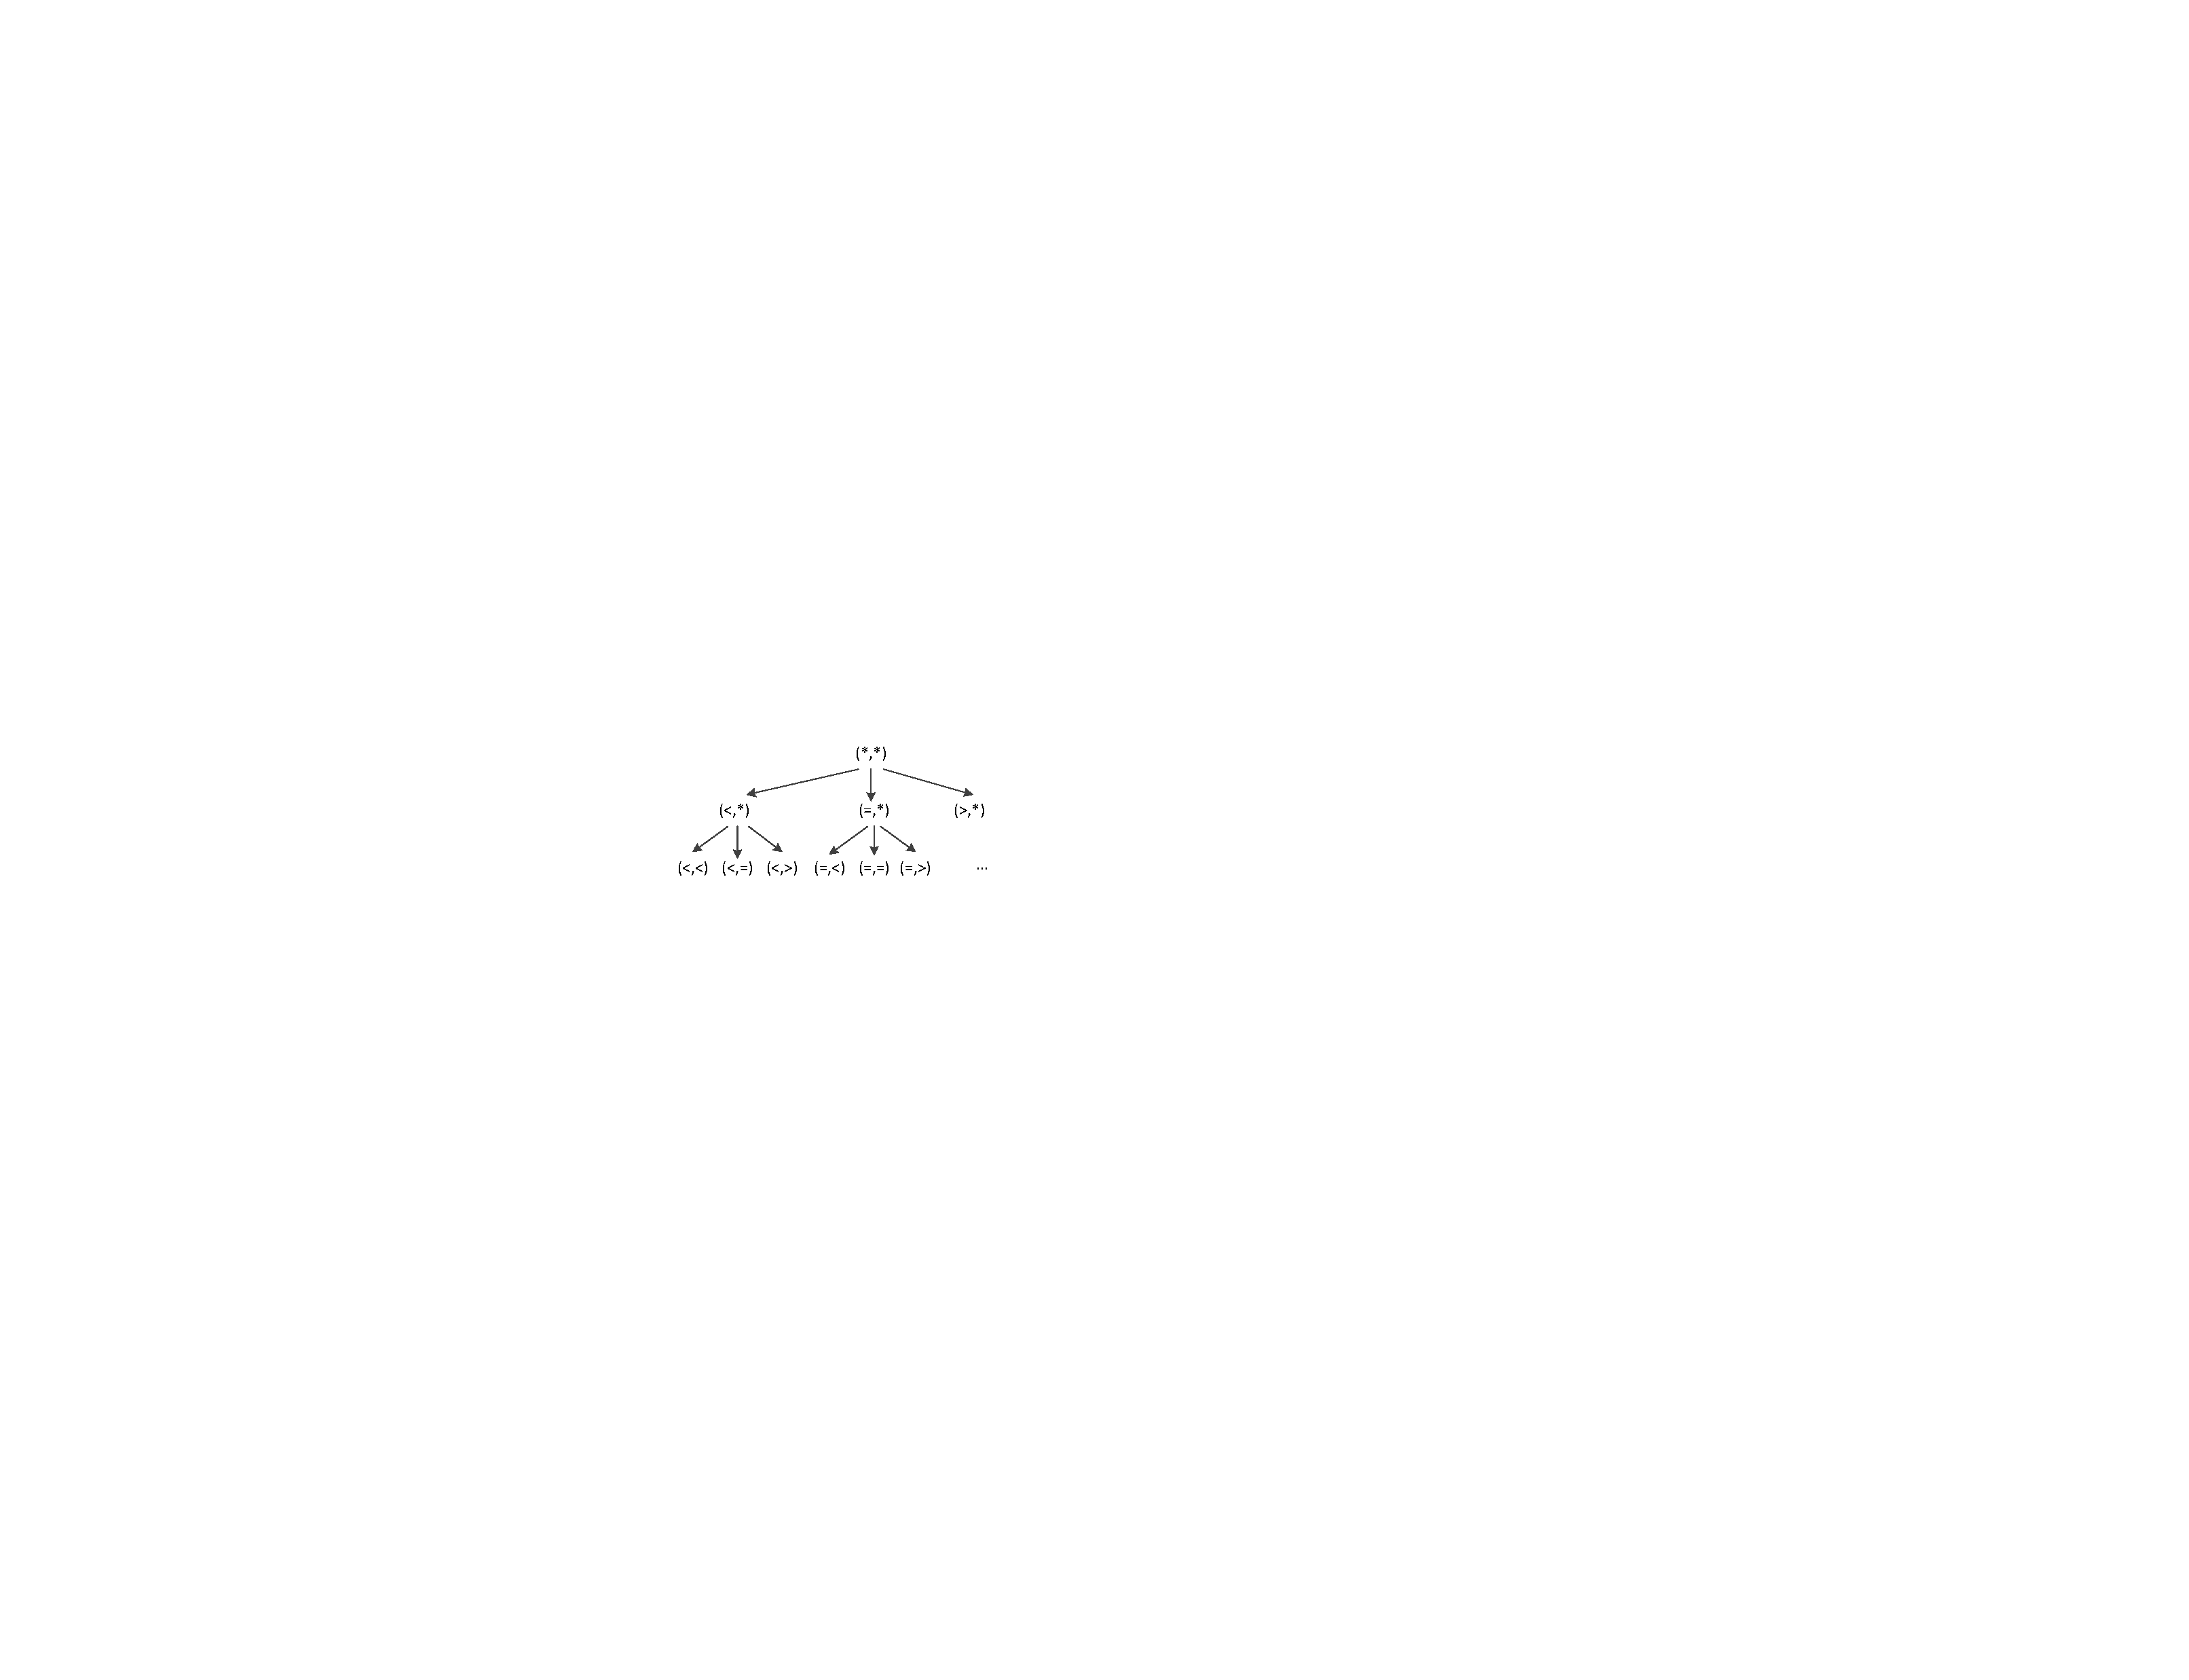
\includegraphics[width=0.6\linewidth]{chap6fig/testingHier.pdf}
\caption{Hierarchy of Dependency Testing for A Two-Level Loop Nest
\label{fig:testingHier}}
\end{center}
\end{figure}
\end{comment}
During the \textit{offline phase}, when the direction vectors based off past runtime profiles are assumed to be true, various transformations are performed. If any of these
assumptions is wrong, the generated accelerator will produce wrong results and should not be run. The \textit{online phase} therefore has to verify all the assumptions. More specifically, it needs to check for the presence of any direction vectors which would
invalidate the instruction reordering the \textit{offline phase} has done. 
There a few main components involved in devising this online checking mechanism:
\begin{enumerate}
    \item Constructing the list of vectors to test.  
    \item Generating C code to test each vector. 
    \item Compiling the vector testing C code into a software routine ($SW_{check}$) or a small hardware engine ($HW_{check}$)
    \item Running $SW_{check}$ or $HW_{check}$ created in the previous step
\end{enumerate}

The first three preparatory steps are all done offline,  after the synthesis of the accelerator. The last part though, is invoked right before the execution of the
accelerator. Its result determines if the original software binary or the generated
hardware accelerator should perform the computation.

To enumerate the direction vectors to be checked, our flow examines all the 
transformations performed during the \textit{offline phase}. These 
%performed during the \textit{offline phase} 
include memory-level parallelism, loop interchange and thread-level parallelization. Loop pipelining is
applied conservatively by Vivado HLS and in most cases, aggressive reordering only happens after separation of memory ports. Its validity check is therefore not invoked independently.  

To ensure memory operations can be reordered or even issued through multiple ports, they need to be completely independent from each other as we have explained previously. The vectors tested during the \texit{offline phase}, (*,*...) or (=...,*...) with barrier insertion, are again included for online testing. For thread-level parallelization,
we have to ensure the level at which the iteration space is split does not carry dependency. That is, for any load-store or store-store pair, the direction vector
cannot have leading $``<"$ at this level. An example is shown in figure~\ref{}.

For loop interchange to be valid, the resultant direction vectors would need to have
leading elements not being $``>"$. To achieve this, we first check if the element being moved outward is $``>"$. If it is, then we check if all the levels outside of it are $``="$. If the test result is affirmative, then the loop interchange has violated the 
original program order and the accelerator should not be invoked. This process
is illustrated in figure~\ref{}.

One efficiency optimization, which
is applicable for both phases, is to replace Banerjee's test with a simple address range test. When two data structures occupied different ranges in the address space, it is
computationally very cheap to just compare the upper and lower bounds of the accessed
addresses.

\begin{comment}

we assume the RTL generation backend, the interconnect and memory subsystem may all be
%aggressively reordering these requests -- by inferring burst accesses or buffering. Therefore, for every pair of accesses whose ordering matters (excluding load-load pair), we check the direction vector (*,*,...), and only continue to execute the accelerator when the test result turns out to be negative. There are also cases where this requirement can be relaxed. In section~\ref{subsec:pmd}, we described how memory barriers are inserted to prevent overly conservative dependency annotation.
%Similarly, in our binary based flow, the online check can be less conservative
%when the ordering of memory operations, each associated with different ports, is partially enforced by barriers.
%An example of this is shown in figure~\ref{fig:withOrWithoutBarrier}. 

In separating 



Memory barriers naturally preclude thread-level parallelization at its level in the loop nest, but memory ports can now be separated as long as the dependency is   carried at or outside the level of insertion. To determine where these barriers
are to be inserted, we uses
 




In a lot of regular computation kernels, data from a multi-dimensional array is read, processed and then written into a different array. Using Banerjee's test, we can obtain negative result for the direction vector (*,*,...), but an easier

Table~\ref{tab:transftest} lists
example tests we need to perform for a three level loop when various transformations were applied.

\begin{table}[htbp]
\caption{Direction Vector Checking for Transformations}
\centering
\begin{tabular}{| c | c | c |  }
  \hline            
 \cline{1-3} 
 Example     & Sequence of Direction  & Description of \\
 Transformations     & Vectors to Disprove & Conditions to Satisfy \\
  %
  %                 & LUT &FFs&  BRAM &  LUT &   FFs      & BRAM   \\
  \hline    
  Separate Memory Ports & (*,*,*)& No dependency\\
  w/o Barriers & &  at every level\\
  \hline
  Separate Memory Ports & (*,*,*) $\rightarrow$ ($>$,*,*) & No dependency below \\  
   with Barriers at level 2 & & the level with barrier\\
  \hline
  Parallelization at & (*,*,*) $\rightarrow$ ($<$,*,*) &\\
  the outermost level & &\\
  \hline     
  Loop Interchange & &\\
 
\hline                                                                                                           

\end{tabular}
\label{tab:transftest}

\end{table}
\end{comment}

%These tests certainly introduce runtime overhead into our system. 
Depending on how much actual computation is going on in the target loop nest, these tests may be incurring a significant runtime overhead, especially if they are run on the processor. On the other hand, these tests are highly parallelizable and can be potentially
offloaded to the hardware completely. In either case, these checks reduce the overall
speed up attainable with the accelerator. %Together with the cost of data transfer, which will be described in section~\ref{dtransfer}, these overheads can nullify the benefit of computation offloading. 
Fortunately, we can statically devise a simple model to
evaluate if the amount of computation justifies the invocation of the validity check and accelerator:
\begin{equation}
& & S_t(I)-H_t(I) >>  D_t
\end{equation}
$S_t(I)$ and $H_t(I)$ are a pair of simple functions estimating the execution time of the loop nest as software binary and hardware accelerator respectively, while $D_t$ denotes the 
runtime overhead of performing parallelization validity check, be it in $SW_{check}$ or $HW_{check}$. $D_t$ does not
vary with the size of the iteration space $I$, while both $S_t$ and $H_t$ are normally simple functions of $I$. 
%given the size of the iteration space. Meanwhile $T_t$ and $D_t$ are functions estimating the time used for data transfer and the parallelism validity check. 
This model is again generated during the offline phase and executed during the online phase. An example model is shown in figure~\ref{}. Evaluating this model takes time as well, but since it can be reduced to a set of quick checks on the loop bounds, its impact ($M$) on execution time would be rather small.


The main steps for the execution of the accelerator-augmented program binaries is illustrated in figure~\ref{pieces-doModel-doOnline-doInvoke}. As the cost model is always evaluated, in the worst case, when
the accelerated version of the loop nest is never executed, there would be a slight increase of $M$ in execution time. It is therefore advisable to only apply our approach to loop nests whose past behavior exposes sufficiently sized iteration space.



%The performance estimates shown in figure~\ref{fig:fpgaparal} do not take into account the data access latency
%if they have to be brought in from off-chip RAM. By performing transformations
%to maximize data reuse, it can increase the ratio of computation v.s. off-chip memory bandwidth usage. 
\subsection{Data Transfer and Address Translation}
\label{dtransfer}
\subsubsection{Communication between CPU and FPGA Memory Spaces}
Another particular important aspect in ensuring the efficient execution of the accelerators is in the management of data transfers. %For the systems we are targeting, the CPU and accelerator can access the shared address space, explicit movement of data may not be necessary. On the other hand, 
As the FPGA are used as an accelerator for binaries executed on CPU, both the source
and final destination of its working datasets are the address space of
the processor. Depending on the actual configuration of the system, the processor memory may or may not be directly accessible by the FPGA, as discussed in section~\ref{chartarg}. We thus need to provide mechanisms to enable
the sharing of data between the two substrates.


For the cases where the FPGA can directly access the 
CPU's address space, which are the primary targets of our flow, the easiest way is to apply the transformation and
optimizations described in chapter~\ref{decoupleChap}. This would
naturally create a set of address generators who pipeline requests into the 
memory subsystem, as can be seen from figure~\ref{show3demuPipeline}. To benefit from the locality-driven optimization we 
have performed, caches can also be inserted between the address outputs and the
off-chip memory. 

In a more complex scenario, the FPGA has its own address space into which program data need to be transferred first before accelerator execution can occur. The output from the accelerator
is also moved explicitly back to the host CPU's address space.
%and a hardware module accessing the CPU memory directly in master mode is implementable. 
Many of the state-of-the-art platforms with this model
are connected to the host through PCI-e connections and both FPGA vendors allow for
OpenCL to be used to program some of these systems. We can thus devise
a mechanism based on OpenCL's data communication model. 
The steps needed include: 
\begin{itemize}
    \item Compute the range of memory addresses to be transferred to and from the FPGA device
    \item Memory allocation on the target FPGA board: $clCreateBuffer$ 
    \item Data transfer to FPGA: $clEnqueueWriteBuffer$
    \item Invoke accelerator: $clEnqueueNDRangeKernel$
    \item Data transfer back to CPU address space: $clEnqueueReadBuffer$
\end{itemize} 

It is worth noting that shared virtual memory (SVM) support has been introduced in OpenCL2.0 where the data movement between the host CPU and the FPGA device can be implicitly handled by the runtime. However, even
in platforms supporting SVM, a buffer is to be allocated explicitly and populated with the appropriate data. For our 
binary based flow, there is still a need to perform the address range computation, memory allocation and kernel(accelerator) invocation. The difference is that now the explicit data transfer between devices gets
replaced by memcpy between the already allocated memory of the original program binary and the SVM buffer just created. 

The analyzability required for coarse grained parallelism discovery 
also enables the \textit{a priori} calculation of the  memory footprint for the accelerated loop nests. As the referenced addresses are always affine functions of the loop indices, for a given part of the iteration space, the boundaries of the accessed range of memory by an instruction can always be
computed. This computation would become another part of the $online$ $phase$, supplying parameters for the actual data movement mechanisms. 


Depending on
the exact computation, the compute of memory ranges and transfer of data
may involve certain trade-offs.
In the best case scenario, every address between the lower and higher boundaries is accessed by the accelerated loop nests. A single memcpy ...
sparse, multiple memcpy may reduce wasted bandwidth for transfer, but increases the overhead in invocation data transfer mechanisms. Application-specific exploration



With the data finally resident in the FPGA's address space, every original access can be translated to a memory reference in the new context by adding/removing an offset. Depending on how the original working
dataset is broken down into memory objects, this offset is computed differently. An example is shown in  figure~\ref{a-memory-reference-get-offseted}. 
In essence, the data transfer mechanism constructs functions for mapping addresses in CPU memory to tuples of (memory object, address) in FPGA memory space. The affine function mapping points in the iteration space to addresses in CPU memory can be composed with these newly constructed function to 


\subsubsection{Handling Virtual Addresses}
When virtual addressing is involved, another layer of complexity is added to the communication between the hardware accelerator and the CPU's memory address space. The CPU's address translation mechanism is normally not accessed by the FPGA, whose outgoing memory requests therefore must use
physical addresses. The generation of addresses by the FPGA accelerator, however, was based off virtual addresses extracted from the software running on the CPU before the accelerator's invocation. It thus becomes necessary to map the virtual addresses generated by the hardware logic to the physical addresses used by the memory subsystem.

In the case where the CPU's memory is not accessible to FPGA
directly and explicit data movement is needed, as just described above, this is less of a problem. One part of the translation happened on the CPU side when the transfer occurs, the virtually referenced data structure get extracted and placed contiguously into the FPGA's physically addressed memory. The remaining part of the translation, as described in part~\ref{dtransfer}, is mere

On the other hand, if the FPGA is to directly generate the addresses used to access the CPU's memory, virtual to physical address translation would need to happen

several different mechanisms might be devised.
Previous projects~\cite{6718414}\cite{7459405}\cite{4042434} 

\begin{comment}

The range of addresses we would like to copy
to the FPGA device needs to be explicitly specified, the size of the


We need to explicitly specify the range of address we would like to copy to the
FPGA device from the CPU
In this case, we rely on the regularity of the memory access patterns in our targeted loop nests to derive a concise representation of the accessed address stream. 




allows us to easily decouple the management of data transfer from the actual computation.
We can derive concise representations of the accessed addresses by the accelerator without actually running it. 
If the FPGA does not have direct access to the CPU memory, then explicit
data transfer is required. This is usually higher cost






Locality driven optimizations performed
described in section~\ref{}




The analyzability required for coarse grained parallelism discovery 
already provided us with 

also
facilitates the calculation of the exact memory footprint for the accelerated computation. 


More specifically, the addresses stream can be 




In addition, many processor centric systems 
use virtual memory to facilitate programming and manage the memory hierarchy, 






The approach described in chapter~\ref{decoupleChap} may be used but provides little advantage for these computation. 






 

%with 
%a particular parallel architecture as the target may be unnecessary. For %instance, vectorizing compilers may perform loop interchange to have 

%An interesting aspect of 

Our parallelization engine attempt to  

\end{comment}

\begin{comment}
The variety of hardware templates gives another dimension in the accelerator design space, in addition to the software domain optimizations like loop interchange, loop tiling etc. 

For a specific loop nest, whose dependence graph is constructed using the information acquired through dependency analysis, there are multiple
possibilities 

As mentioned in section~\ref{sec:fdtp}, we use Banerjee's tests to find 
direction vectors between different statements in the loop nest. There are 
a few additional techniques employed to make runtime check cheaper





One particular important aspect, in ensuring the efficient execution of the accelerators, is in the management of data transfers. 
The regularity of the memory access patterns in our targeted loop nests
allow us  to easily decouple the transfer of data from the computation. 
The analyzability required for coarse grained parallelism discovery also
facilitates the calculation of the exact memory footprint for the accelerated computation. More specifically, the addresses stream can be 


The approach described in chapter~\ref{decoupleChap} may be used but provides little advantage for these computation. 
\end{comment}

\begin{comment}
At a high level, the approach we are proposing in accelerating program binaries
can be divided into two phases. For an acceleratable loop nest, we first examine
it's past execution profile to extract necessary information to perform dependency analysis offline. After obtaining the dependency direction vectors between statements, we can then perform parallelization and the actual accelerator synthesis. 
Now, whether the generated accelerator is consistent
with the semantics of the original program depends on if the dependency
testing results remain true when the actual execution happens. This is our
second phase, where an online check is performed to confirm the validity
of the assumed parallelism.
\end{comment}








\newpage


\newpage
\newpage
\section{Accelerator Integration through Binary Instrumentation}
\newpage

\section{Experimental Evaluation }
\label{biev}






\section{Discussion and Future Work}
If OpenCL is actually being used to perform hardware generation, the analysis work we have done to extract coarse grained parallelism would still work.
At the same time...packaging the transferred data into the memory objects can affect the final performance as well. Having everything in a single 
object in openCL's global memory space ------ not good, less memory level parallelism even though the data transfer between host and FPGA platform
is easier. 




\begin{comment}

%When the input data are changed, the generated accelerator may actually violate
%the semantics of the program. As we have mentioned in section~\ref{sec:cfbba},
%a verifying function is invoked before the accelerator to ensure the correctness
%of the overall execution. Besides, the \textit{online} phase also need to 



%Now the dependency testing results and the subsequent parallelization are a reflection of the programs' past behavior which
%may or may not hold true when the input data are changed. This is when the
%second phase 






%To actually obtain the direction vectors from equation~\ref{adioeq},
%we use Banerjee's approach~\cite{banerjee}.
%To actually solve equation~\ref{adioeq}, we use Banerjee's approach~\cite{}, which find the solution for the non-integer relaxation of the ILP formulation. It does
%which requires constant coefficients. 
%As the coefficients in the equation are not known from the static binary, our flow examines the runtime profiles to extract the values.
%The direction vectors thus obtained can be used evaluate how much coarse
%grained parallelism 



%Their values are extracted from the runtime profile of the programs.
Therefore, the dependency testing results are a reflection of the programs'
past behavior, which may or may not hold true when the input data are changed.
However, given a new set of runtime variables, the amount of computation needed to confirm the results of earlier dependency testing would be constant. This is not hard to see as the size of the problem formulated 
does not depend on the actual values of the coefficients. We now have the computation which has $O(1)$ cost yet guarantees the validity of the extracted
parallelism.


Meanwhile, it is worth noting that Banerjee's inequality only tests for existence of \textit{ real} solutions for the Diophantine's equations. Since it only tackles the non-integer relaxation of the ILP formulation, the results obtained are conservative. False dependencies are reported if all the real solutions are non-integral. More accurate tests like~\cite{omega} find integer solutions but are more costly. As we are
going to perform the test using runtime data when the accelerator is actually
being invoked, the faster, though more pessimistic, approach is preferred.





To actually obtain the direction vectors from equation~\ref{adioeq},
we use Banerjee's approach~\cite{banerjee}.
%To actually solve equation~\ref{adioeq}, we use Banerjee's approach~\cite{}, which find the solution for the non-integer relaxation of the ILP formulation. It does
%which requires constant coefficients. 
As mentioned in section~\ref{sec:cfbba}, the coefficients in the equation, despite being unchanged during the loop execution, are not known from the static binary. Our flow examines the runtime profiles to extract the coefficient values
%Their values are extracted from the runtime profile of the programs.
Therefore, the dependency testing results are a reflection of the programs'
past behavior, which may or may not hold true when the input data are changed.
However, given a new set of runtime variables, the amount of computation needed to confirm the results of earlier dependency testing would be constant. This is not hard to see as the size of the problem formulated 
does not depend on the actual values of the coefficients. We now have the computation which has $O(1)$ cost yet guarantees the validity of the extracted
parallelism.


Meanwhile, it is worth noting that Banerjee's inequality only tests for existence of \textit{ real} solutions for the Diophantine's equations. Since it only tackles the non-integer relaxation of the ILP formulation, the results obtained are conservative. It will never report lack of dependencies when one exists,  but may report false dependencies -- when all the real solutions are non-integral. More accurate tests like~\cite{omega} find integer solutions but are more costly. As we are
going to perform the test using runtime data when the accelerator is actually
being invoked, the faster, though more pessimistic, approach is preferred.







As we mentioned in section~\ref{sec:cfbba}, for loops with analyzable memory accesses, we can perform run time check to validate parallelization we performed in creating the accelerators. This 

As we use past execution profiles to extract parallelism and then perform runtime checks to confirm the validity of our parallelization, our approach
in accelerating program binaries can be divided into two phases. The offline
phase (compile time) consists of dependency analysis, accelerator synthesis and accelerator driver generation. Meanwhile, the parallelism validity check, data transfer and invocation of the accelerator are all performed during the online phase (run time). Being part of the driver, the actual code segments to perform validity check and data transfer are all generated during compile time. As our primary objective is to boost the performance of the accelerated loop nests, the flow tries to create simple and fast run time code whenever it, at the expense
of the compilation time and at times, the accuracy of the run time mechanisms.
\end{comment}
\chapter{Conclusion}
\label{concluChap}



% \appendix
% \chapter{More Monticello Candidates}

\printbibliography

\end{document}
